% Options for packages loaded elsewhere
\PassOptionsToPackage{unicode}{hyperref}
\PassOptionsToPackage{hyphens}{url}
\documentclass[
]{article}
\usepackage{xcolor}
\usepackage[margin=1in]{geometry}
\usepackage{amsmath,amssymb}
\setcounter{secnumdepth}{-\maxdimen} % remove section numbering
\usepackage{iftex}
\ifPDFTeX
  \usepackage[T1]{fontenc}
  \usepackage[utf8]{inputenc}
  \usepackage{textcomp} % provide euro and other symbols
\else % if luatex or xetex
  \usepackage{unicode-math} % this also loads fontspec
  \defaultfontfeatures{Scale=MatchLowercase}
  \defaultfontfeatures[\rmfamily]{Ligatures=TeX,Scale=1}
\fi
\usepackage{lmodern}
\ifPDFTeX\else
  % xetex/luatex font selection
\fi
% Use upquote if available, for straight quotes in verbatim environments
\IfFileExists{upquote.sty}{\usepackage{upquote}}{}
\IfFileExists{microtype.sty}{% use microtype if available
  \usepackage[]{microtype}
  \UseMicrotypeSet[protrusion]{basicmath} % disable protrusion for tt fonts
}{}
\makeatletter
\@ifundefined{KOMAClassName}{% if non-KOMA class
  \IfFileExists{parskip.sty}{%
    \usepackage{parskip}
  }{% else
    \setlength{\parindent}{0pt}
    \setlength{\parskip}{6pt plus 2pt minus 1pt}}
}{% if KOMA class
  \KOMAoptions{parskip=half}}
\makeatother
\usepackage{color}
\usepackage{fancyvrb}
\newcommand{\VerbBar}{|}
\newcommand{\VERB}{\Verb[commandchars=\\\{\}]}
\DefineVerbatimEnvironment{Highlighting}{Verbatim}{commandchars=\\\{\}}
% Add ',fontsize=\small' for more characters per line
\usepackage{framed}
\definecolor{shadecolor}{RGB}{248,248,248}
\newenvironment{Shaded}{\begin{snugshade}}{\end{snugshade}}
\newcommand{\AlertTok}[1]{\textcolor[rgb]{0.94,0.16,0.16}{#1}}
\newcommand{\AnnotationTok}[1]{\textcolor[rgb]{0.56,0.35,0.01}{\textbf{\textit{#1}}}}
\newcommand{\AttributeTok}[1]{\textcolor[rgb]{0.13,0.29,0.53}{#1}}
\newcommand{\BaseNTok}[1]{\textcolor[rgb]{0.00,0.00,0.81}{#1}}
\newcommand{\BuiltInTok}[1]{#1}
\newcommand{\CharTok}[1]{\textcolor[rgb]{0.31,0.60,0.02}{#1}}
\newcommand{\CommentTok}[1]{\textcolor[rgb]{0.56,0.35,0.01}{\textit{#1}}}
\newcommand{\CommentVarTok}[1]{\textcolor[rgb]{0.56,0.35,0.01}{\textbf{\textit{#1}}}}
\newcommand{\ConstantTok}[1]{\textcolor[rgb]{0.56,0.35,0.01}{#1}}
\newcommand{\ControlFlowTok}[1]{\textcolor[rgb]{0.13,0.29,0.53}{\textbf{#1}}}
\newcommand{\DataTypeTok}[1]{\textcolor[rgb]{0.13,0.29,0.53}{#1}}
\newcommand{\DecValTok}[1]{\textcolor[rgb]{0.00,0.00,0.81}{#1}}
\newcommand{\DocumentationTok}[1]{\textcolor[rgb]{0.56,0.35,0.01}{\textbf{\textit{#1}}}}
\newcommand{\ErrorTok}[1]{\textcolor[rgb]{0.64,0.00,0.00}{\textbf{#1}}}
\newcommand{\ExtensionTok}[1]{#1}
\newcommand{\FloatTok}[1]{\textcolor[rgb]{0.00,0.00,0.81}{#1}}
\newcommand{\FunctionTok}[1]{\textcolor[rgb]{0.13,0.29,0.53}{\textbf{#1}}}
\newcommand{\ImportTok}[1]{#1}
\newcommand{\InformationTok}[1]{\textcolor[rgb]{0.56,0.35,0.01}{\textbf{\textit{#1}}}}
\newcommand{\KeywordTok}[1]{\textcolor[rgb]{0.13,0.29,0.53}{\textbf{#1}}}
\newcommand{\NormalTok}[1]{#1}
\newcommand{\OperatorTok}[1]{\textcolor[rgb]{0.81,0.36,0.00}{\textbf{#1}}}
\newcommand{\OtherTok}[1]{\textcolor[rgb]{0.56,0.35,0.01}{#1}}
\newcommand{\PreprocessorTok}[1]{\textcolor[rgb]{0.56,0.35,0.01}{\textit{#1}}}
\newcommand{\RegionMarkerTok}[1]{#1}
\newcommand{\SpecialCharTok}[1]{\textcolor[rgb]{0.81,0.36,0.00}{\textbf{#1}}}
\newcommand{\SpecialStringTok}[1]{\textcolor[rgb]{0.31,0.60,0.02}{#1}}
\newcommand{\StringTok}[1]{\textcolor[rgb]{0.31,0.60,0.02}{#1}}
\newcommand{\VariableTok}[1]{\textcolor[rgb]{0.00,0.00,0.00}{#1}}
\newcommand{\VerbatimStringTok}[1]{\textcolor[rgb]{0.31,0.60,0.02}{#1}}
\newcommand{\WarningTok}[1]{\textcolor[rgb]{0.56,0.35,0.01}{\textbf{\textit{#1}}}}
\usepackage{graphicx}
\makeatletter
\newsavebox\pandoc@box
\newcommand*\pandocbounded[1]{% scales image to fit in text height/width
  \sbox\pandoc@box{#1}%
  \Gscale@div\@tempa{\textheight}{\dimexpr\ht\pandoc@box+\dp\pandoc@box\relax}%
  \Gscale@div\@tempb{\linewidth}{\wd\pandoc@box}%
  \ifdim\@tempb\p@<\@tempa\p@\let\@tempa\@tempb\fi% select the smaller of both
  \ifdim\@tempa\p@<\p@\scalebox{\@tempa}{\usebox\pandoc@box}%
  \else\usebox{\pandoc@box}%
  \fi%
}
% Set default figure placement to htbp
\def\fps@figure{htbp}
\makeatother
\setlength{\emergencystretch}{3em} % prevent overfull lines
\providecommand{\tightlist}{%
  \setlength{\itemsep}{0pt}\setlength{\parskip}{0pt}}
\usepackage{bookmark}
\IfFileExists{xurl.sty}{\usepackage{xurl}}{} % add URL line breaks if available
\urlstyle{same}
\hypersetup{
  pdftitle={Final Project Part 2},
  pdfauthor={Maximilien Filion - 20598645,; Aneesh Kaura - 66832304,; Monica Mihailescu - 47409289},
  hidelinks,
  pdfcreator={LaTeX via pandoc}}

\title{Final Project Part 2}
\author{Maximilien Filion - 20598645, \and Aneesh Kaura -
66832304, \and Monica Mihailescu - 47409289}
\date{2025-11-17}

\begin{document}
\maketitle

\section{============================================================================}\label{section}

\section{RNA-seq Analysis Template: Clustering and Differential
Expression}\label{rna-seq-analysis-template-clustering-and-differential-expression}

\section{============================================================================}\label{section-1}

\section{This template provides a structured framework for comprehensive
gene}\label{this-template-provides-a-structured-framework-for-comprehensive-gene}

\section{expression analysis from preprocessing through clinical
validation}\label{expression-analysis-from-preprocessing-through-clinical-validation}

\section{============================================================================}\label{section-2}

\section{Load required libraries}\label{load-required-libraries}

\begin{Shaded}
\begin{Highlighting}[]
\CommentTok{\#if (!requireNamespace("BiocManager", quietly = TRUE))}
\CommentTok{\#     install.packages("BiocManager")}
\CommentTok{\# BiocManager::install("org.Hs.eg.db")}
\CommentTok{\# BiocManager::install("AnnotationDbi") }

\CommentTok{\# Install clusterProfiler properly}
\CommentTok{\#BiocManager::install("clusterProfiler", ask = FALSE, update = FALSE)}

\CommentTok{\#BiocManager::install("DOSE")}
\CommentTok{\#BiocManager::install("pathview") }

\FunctionTok{library}\NormalTok{(clusterProfiler)}
\end{Highlighting}
\end{Shaded}

\begin{verbatim}
## 
\end{verbatim}

\begin{verbatim}
## clusterProfiler v4.16.0 Learn more at https://yulab-smu.top/contribution-knowledge-mining/
## 
## Please cite:
## 
## Guangchuang Yu, Li-Gen Wang, Yanyan Han and Qing-Yu He.
## clusterProfiler: an R package for comparing biological themes among
## gene clusters. OMICS: A Journal of Integrative Biology. 2012,
## 16(5):284-287
\end{verbatim}

\begin{verbatim}
## 
## Attaching package: 'clusterProfiler'
\end{verbatim}

\begin{verbatim}
## The following object is masked from 'package:stats':
## 
##     filter
\end{verbatim}

\begin{Shaded}
\begin{Highlighting}[]
\FunctionTok{library}\NormalTok{(AnnotationDbi)}
\end{Highlighting}
\end{Shaded}

\begin{verbatim}
## Loading required package: stats4
\end{verbatim}

\begin{verbatim}
## Loading required package: BiocGenerics
\end{verbatim}

\begin{verbatim}
## Loading required package: generics
\end{verbatim}

\begin{verbatim}
## 
## Attaching package: 'generics'
\end{verbatim}

\begin{verbatim}
## The following objects are masked from 'package:base':
## 
##     as.difftime, as.factor, as.ordered, intersect, is.element, setdiff,
##     setequal, union
\end{verbatim}

\begin{verbatim}
## 
## Attaching package: 'BiocGenerics'
\end{verbatim}

\begin{verbatim}
## The following objects are masked from 'package:stats':
## 
##     IQR, mad, sd, var, xtabs
\end{verbatim}

\begin{verbatim}
## The following objects are masked from 'package:base':
## 
##     anyDuplicated, aperm, append, as.data.frame, basename, cbind,
##     colnames, dirname, do.call, duplicated, eval, evalq, Filter, Find,
##     get, grep, grepl, is.unsorted, lapply, Map, mapply, match, mget,
##     order, paste, pmax, pmax.int, pmin, pmin.int, Position, rank,
##     rbind, Reduce, rownames, sapply, saveRDS, table, tapply, unique,
##     unsplit, which.max, which.min
\end{verbatim}

\begin{verbatim}
## Loading required package: Biobase
\end{verbatim}

\begin{verbatim}
## Welcome to Bioconductor
## 
##     Vignettes contain introductory material; view with
##     'browseVignettes()'. To cite Bioconductor, see
##     'citation("Biobase")', and for packages 'citation("pkgname")'.
\end{verbatim}

\begin{verbatim}
## Loading required package: IRanges
\end{verbatim}

\begin{verbatim}
## Loading required package: S4Vectors
\end{verbatim}

\begin{verbatim}
## 
## Attaching package: 'S4Vectors'
\end{verbatim}

\begin{verbatim}
## The following object is masked from 'package:clusterProfiler':
## 
##     rename
\end{verbatim}

\begin{verbatim}
## The following object is masked from 'package:utils':
## 
##     findMatches
\end{verbatim}

\begin{verbatim}
## The following objects are masked from 'package:base':
## 
##     expand.grid, I, unname
\end{verbatim}

\begin{verbatim}
## 
## Attaching package: 'IRanges'
\end{verbatim}

\begin{verbatim}
## The following object is masked from 'package:clusterProfiler':
## 
##     slice
\end{verbatim}

\begin{verbatim}
## The following object is masked from 'package:grDevices':
## 
##     windows
\end{verbatim}

\begin{verbatim}
## 
## Attaching package: 'AnnotationDbi'
\end{verbatim}

\begin{verbatim}
## The following object is masked from 'package:clusterProfiler':
## 
##     select
\end{verbatim}

\begin{Shaded}
\begin{Highlighting}[]
\FunctionTok{library}\NormalTok{(DESeq2)}
\end{Highlighting}
\end{Shaded}

\begin{verbatim}
## Loading required package: GenomicRanges
\end{verbatim}

\begin{verbatim}
## Loading required package: GenomeInfoDb
\end{verbatim}

\begin{verbatim}
## Loading required package: SummarizedExperiment
\end{verbatim}

\begin{verbatim}
## Loading required package: MatrixGenerics
\end{verbatim}

\begin{verbatim}
## Loading required package: matrixStats
\end{verbatim}

\begin{verbatim}
## 
## Attaching package: 'matrixStats'
\end{verbatim}

\begin{verbatim}
## The following objects are masked from 'package:Biobase':
## 
##     anyMissing, rowMedians
\end{verbatim}

\begin{verbatim}
## 
## Attaching package: 'MatrixGenerics'
\end{verbatim}

\begin{verbatim}
## The following objects are masked from 'package:matrixStats':
## 
##     colAlls, colAnyNAs, colAnys, colAvgsPerRowSet, colCollapse,
##     colCounts, colCummaxs, colCummins, colCumprods, colCumsums,
##     colDiffs, colIQRDiffs, colIQRs, colLogSumExps, colMadDiffs,
##     colMads, colMaxs, colMeans2, colMedians, colMins, colOrderStats,
##     colProds, colQuantiles, colRanges, colRanks, colSdDiffs, colSds,
##     colSums2, colTabulates, colVarDiffs, colVars, colWeightedMads,
##     colWeightedMeans, colWeightedMedians, colWeightedSds,
##     colWeightedVars, rowAlls, rowAnyNAs, rowAnys, rowAvgsPerColSet,
##     rowCollapse, rowCounts, rowCummaxs, rowCummins, rowCumprods,
##     rowCumsums, rowDiffs, rowIQRDiffs, rowIQRs, rowLogSumExps,
##     rowMadDiffs, rowMads, rowMaxs, rowMeans2, rowMedians, rowMins,
##     rowOrderStats, rowProds, rowQuantiles, rowRanges, rowRanks,
##     rowSdDiffs, rowSds, rowSums2, rowTabulates, rowVarDiffs, rowVars,
##     rowWeightedMads, rowWeightedMeans, rowWeightedMedians,
##     rowWeightedSds, rowWeightedVars
\end{verbatim}

\begin{verbatim}
## The following object is masked from 'package:Biobase':
## 
##     rowMedians
\end{verbatim}

\begin{Shaded}
\begin{Highlighting}[]
\FunctionTok{library}\NormalTok{(pheatmap)}
\end{Highlighting}
\end{Shaded}

\begin{verbatim}
## Warning: package 'pheatmap' was built under R version 4.5.2
\end{verbatim}

\begin{Shaded}
\begin{Highlighting}[]
\FunctionTok{library}\NormalTok{(ggplot2)}
\end{Highlighting}
\end{Shaded}

\begin{verbatim}
## Warning: package 'ggplot2' was built under R version 4.5.2
\end{verbatim}

\begin{Shaded}
\begin{Highlighting}[]
\FunctionTok{library}\NormalTok{(cluster)}
\FunctionTok{library}\NormalTok{(survival)}
\FunctionTok{library}\NormalTok{(survminer)}
\end{Highlighting}
\end{Shaded}

\begin{verbatim}
## Loading required package: ggpubr
\end{verbatim}

\begin{verbatim}
## 
## Attaching package: 'survminer'
\end{verbatim}

\begin{verbatim}
## The following object is masked from 'package:survival':
## 
##     myeloma
\end{verbatim}

\begin{Shaded}
\begin{Highlighting}[]
\CommentTok{\#library(clusterProfiler)}
\FunctionTok{library}\NormalTok{(org.Hs.eg.db) }\CommentTok{\# Contains human gene annotations}
\end{Highlighting}
\end{Shaded}

\begin{verbatim}
## 
\end{verbatim}

\begin{Shaded}
\begin{Highlighting}[]
\FunctionTok{library}\NormalTok{(dplyr)}
\end{Highlighting}
\end{Shaded}

\begin{verbatim}
## 
## Attaching package: 'dplyr'
\end{verbatim}

\begin{verbatim}
## The following object is masked from 'package:matrixStats':
## 
##     count
\end{verbatim}

\begin{verbatim}
## The following objects are masked from 'package:GenomicRanges':
## 
##     intersect, setdiff, union
\end{verbatim}

\begin{verbatim}
## The following object is masked from 'package:GenomeInfoDb':
## 
##     intersect
\end{verbatim}

\begin{verbatim}
## The following object is masked from 'package:AnnotationDbi':
## 
##     select
\end{verbatim}

\begin{verbatim}
## The following objects are masked from 'package:IRanges':
## 
##     collapse, desc, intersect, setdiff, slice, union
\end{verbatim}

\begin{verbatim}
## The following objects are masked from 'package:S4Vectors':
## 
##     first, intersect, rename, setdiff, setequal, union
\end{verbatim}

\begin{verbatim}
## The following object is masked from 'package:Biobase':
## 
##     combine
\end{verbatim}

\begin{verbatim}
## The following objects are masked from 'package:BiocGenerics':
## 
##     combine, intersect, setdiff, setequal, union
\end{verbatim}

\begin{verbatim}
## The following object is masked from 'package:generics':
## 
##     explain
\end{verbatim}

\begin{verbatim}
## The following objects are masked from 'package:stats':
## 
##     filter, lag
\end{verbatim}

\begin{verbatim}
## The following objects are masked from 'package:base':
## 
##     intersect, setdiff, setequal, union
\end{verbatim}

\begin{Shaded}
\begin{Highlighting}[]
\FunctionTok{library}\NormalTok{(tibble)}
\FunctionTok{library}\NormalTok{(biomaRt)   }
\end{Highlighting}
\end{Shaded}

set.seed(1)

\section{============================================================================}\label{section-3}

\section{STEP 1: DATA LOADING AND INITIAL
SETUP}\label{step-1-data-loading-and-initial-setup}

\section{============================================================================}\label{section-4}

\section{Load the data files}\label{load-the-data-files}

\section{- count\_matrix: raw counts (genes x
samples)}\label{count_matrix-raw-counts-genes-x-samples}

\section{- clinical\_data: patient clinical
information}\label{clinical_data-patient-clinical-information}

\section{- mutation\_data: mutation status for each
patient}\label{mutation_data-mutation-status-for-each-patient}

\begin{Shaded}
\begin{Highlighting}[]
\CommentTok{\#Load the data (from lab 7)}
\NormalTok{RNAseq\_KIRC }\OtherTok{\textless{}{-}} \FunctionTok{read.csv}\NormalTok{(}\StringTok{"RNAseq\_KIRC.csv"}\NormalTok{)}
\NormalTok{data\_clinical\_patient }\OtherTok{\textless{}{-}} \FunctionTok{read.delim}\NormalTok{(}\StringTok{"data\_clinical\_patient.txt"}\NormalTok{, }\AttributeTok{header =} \ConstantTok{TRUE}\NormalTok{, }\AttributeTok{sep =} \StringTok{"}\SpecialCharTok{\textbackslash{}t}\StringTok{"}\NormalTok{, }\AttributeTok{skip =} \DecValTok{4}\NormalTok{)}
\NormalTok{data\_mutations }\OtherTok{\textless{}{-}} \FunctionTok{read.delim}\NormalTok{(}\StringTok{"data\_mutations.txt"}\NormalTok{, }\AttributeTok{header =} \ConstantTok{TRUE}\NormalTok{, }\AttributeTok{sep =} \StringTok{"}\SpecialCharTok{\textbackslash{}t}\StringTok{"}\NormalTok{, }\AttributeTok{stringsAsFactors =} \ConstantTok{FALSE}\NormalTok{)}
\end{Highlighting}
\end{Shaded}

\begin{Shaded}
\begin{Highlighting}[]
\FunctionTok{head}\NormalTok{(RNAseq\_KIRC)}
\end{Highlighting}
\end{Shaded}

\begin{verbatim}
##                    X TCGA.BP.4756.01A.01R.1289.07 TCGA.BP.4999.01A.01R.1334.07
## 1 ENSG00000000003.15                         3290                         4357
## 2  ENSG00000000005.6                            7                            6
## 3 ENSG00000000419.13                         1157                         1749
## 4 ENSG00000000457.14                          929                          836
## 5 ENSG00000000460.17                          196                          332
## 6 ENSG00000000938.13                          789                         1295
##   TCGA.CJ.5684.01A.11R.1541.07 TCGA.B0.5692.01A.11R.1541.07
## 1                         2863                         1621
## 2                           39                          169
## 3                         1178                         1033
## 4                          655                          508
## 5                          113                          161
## 6                          781                         1128
##   TCGA.BP.4988.01A.01R.1334.07 TCGA.BP.5010.01A.02R.1420.07
## 1                         1055                         2117
## 2                            8                          104
## 3                         1202                          775
## 4                          814                          387
## 5                          591                           89
## 6                         8750                          775
##   TCGA.CZ.5451.01A.01R.1503.07 TCGA.CJ.4899.01A.01R.1334.07
## 1                         2777                         2932
## 2                           83                           22
## 3                          964                         1986
## 4                          504                         1174
## 5                          142                          361
## 6                         1094                         1973
##   TCGA.CW.5590.01A.01R.1541.07 TCGA.B8.5545.01A.01R.1672.07
## 1                         4446                         3291
## 2                          192                           15
## 3                         1137                         1347
## 4                          680                          747
## 5                          169                          257
## 6                          843                          845
##   TCGA.B2.5641.11A.01R.1541.07 TCGA.CJ.4902.01A.01R.1426.07
## 1                         6566                         5901
## 2                           35                          931
## 3                         1075                         1860
## 4                          874                         1046
## 5                          133                          376
## 6                          198                         1923
##   TCGA.B0.5102.01A.01R.1420.07 TCGA.BP.4801.01A.02R.1420.07
## 1                         4813                         2420
## 2                            7                           18
## 3                         1491                         1297
## 4                          381                          573
## 5                          124                          195
## 6                          739                         1287
##   TCGA.CZ.5460.01A.01R.1503.07 TCGA.BP.4347.01A.01R.1289.07
## 1                         2285                         2789
## 2                           22                           26
## 3                         1594                         2026
## 4                          487                          902
## 5                          154                          300
## 6                         1157                         1270
##   TCGA.CJ.4635.01A.02R.1305.07 TCGA.A3.A6NJ.01A.12R.A33J.07
## 1                         3279                         1766
## 2                            2                            2
## 3                         1129                         1510
## 4                          588                          522
## 5                          197                          155
## 6                          951                         1784
##   TCGA.BP.4962.01A.01R.1334.07 TCGA.B4.5834.01A.11R.1672.07
## 1                         1724                         4543
## 2                           16                           34
## 3                         1709                         1669
## 4                          449                          914
## 5                          148                          225
## 6                         1103                          987
##   TCGA.BP.4963.01A.01R.1334.07 TCGA.B0.5116.01A.02R.1420.07
## 1                         2741                         7189
## 2                            4                            4
## 3                         1108                         1562
## 4                          730                          597
## 5                          222                          204
## 6                         1910                          249
##   TCGA.B2.4101.01A.02R.1277.07 TCGA.B0.5707.01A.11R.1541.07
## 1                         1984                         3581
## 2                            3                            5
## 3                         1173                         1888
## 4                          684                          329
## 5                          215                          102
## 6                         1725                          754
##   TCGA.B0.5108.01A.01R.1420.07 TCGA.A3.3313.01A.02R.1325.07
## 1                         2038                         3187
## 2                            1                            0
## 3                         1435                         1475
## 4                          720                          706
## 5                          244                          230
## 6                         2032                          311
##   TCGA.B0.4843.01A.01R.1277.07 TCGA.CW.5585.11A.01R.1541.07
## 1                         1651                         6857
## 2                            0                          238
## 3                          533                         1791
## 4                          376                          742
## 5                           97                          128
## 6                          607                          216
##   TCGA.CW.5585.01A.01R.1541.07 TCGA.B8.A8YJ.01A.13R.A39I.07
## 1                         3492                         1497
## 2                           24                            8
## 3                         1423                         1191
## 4                          969                          436
## 5                          180                          173
## 6                          965                         1421
##   TCGA.B8.5164.01A.01R.1420.07 TCGA.CJ.4637.01A.02R.1325.07
## 1                         3557                         1181
## 2                           47                            1
## 3                         1543                         1808
## 4                          867                          907
## 5                          319                          359
## 6                         1744                          991
##   TCGA.B0.4841.01A.01R.1277.07 TCGA.CJ.4870.01A.01R.1305.07
## 1                          808                         3314
## 2                           48                           62
## 3                          348                          959
## 4                          179                          391
## 5                           38                          119
## 6                          477                         1302
##   TCGA.B0.5400.01A.01R.1503.07 TCGA.BP.4784.01A.01R.1305.07
## 1                         1772                         4165
## 2                           10                            8
## 3                         1326                         1431
## 4                          337                          639
## 5                          123                          160
## 6                         1165                          320
##   TCGA.A3.3363.01A.01R.0864.07 TCGA.B8.4621.01A.01R.1503.07
## 1                         5857                         4660
## 2                            4                           12
## 3                         2173                         1808
## 4                         1207                          552
## 5                          241                          175
## 6                          638                         2236
##   TCGA.B0.5690.01A.11R.1541.07 TCGA.B0.5702.01A.11R.1541.07
## 1                         2164                          776
## 2                           47                            5
## 3                         1120                           40
## 4                          636                           78
## 5                          184                            1
## 6                         2025                          272
##   TCGA.B0.5083.01A.02R.1420.07 TCGA.B0.4688.01A.01R.1277.07
## 1                         2873                         8186
## 2                            0                            0
## 3                         1596                          737
## 4                          348                          614
## 5                           82                          666
## 6                          544                          502
##   TCGA.BP.4781.01A.01R.1305.07 TCGA.B4.5832.01A.11R.1672.07
## 1                         3992                         5500
## 2                            5                            6
## 3                         1422                         2877
## 4                          702                          394
## 5                          239                          136
## 6                          980                          129
##   TCGA.BP.4766.01A.01R.1289.07 TCGA.B0.5121.01A.02R.1420.07
## 1                         3235                         2607
## 2                           13                           31
## 3                         1604                         1167
## 4                          935                          567
## 5                          278                          175
## 6                         2248                         1791
##   TCGA.CJ.4872.01A.01R.1305.07 TCGA.CZ.4863.11A.01R.1503.07
## 1                         3230                        12069
## 2                            8                           24
## 3                         1453                         2807
## 4                          651                         1315
## 5                          217                          267
## 6                         1263                          580
##   TCGA.B2.5633.01B.04R.A277.07 TCGA.CW.5580.11A.02R.1672.07
## 1                          930                        11441
## 2                           24                          100
## 3                          450                         1956
## 4                          691                         1211
## 5                          398                          184
## 6                          485                          670
##   TCGA.A3.3317.01A.02R.1325.07 TCGA.CZ.4853.01A.01R.1426.07
## 1                         2866                         3537
## 2                         5746                           21
## 3                         1388                         1464
## 4                          869                          809
## 5                          271                          218
## 6                         1129                          683
##   TCGA.BP.4991.01A.01R.1334.07 TCGA.CZ.5986.11A.01R.1672.07
## 1                         3645                         5549
## 2                           13                           97
## 3                         1769                         1218
## 4                         1020                          721
## 5                          370                           96
## 6                         1667                          205
##   TCGA.B0.4691.01A.01R.1277.07 TCGA.CZ.5463.11A.01R.1503.07
## 1                         2718                        13291
## 2                           32                           96
## 3                         1572                         2184
## 4                          467                         1153
## 5                          143                          220
## 6                          809                          621
##   TCGA.B0.5713.01A.11R.1672.07 TCGA.CJ.6032.01A.11R.1672.07
## 1                         2846                         3211
## 2                           90                           35
## 3                         1663                         1837
## 4                          710                          450
## 5                          185                          176
## 6                         1443                         1121
##   TCGA.B0.5709.11A.01R.1541.07 TCGA.B8.4146.01B.11R.1672.07
## 1                         6903                         5898
## 2                          188                           38
## 3                         1945                         3222
## 4                          943                          910
## 5                          160                          358
## 6                          378                          478
##   TCGA.AK.3445.01A.02R.1277.07 TCGA.A3.3335.01A.01R.0864.07
## 1                         4107                         2413
## 2                            1                           16
## 3                         1324                         1594
## 4                          457                          383
## 5                          231                          148
## 6                          456                          618
##   TCGA.BP.4342.01A.01R.1289.07 TCGA.B8.5163.01A.01R.1420.07
## 1                         2833                         4895
## 2                            2                            7
## 3                         1579                         2094
## 4                         1149                          849
## 5                          265                          415
## 6                          708                          679
##   TCGA.B0.5092.01A.01R.1420.07 TCGA.B0.4703.01A.01R.1277.07
## 1                         1127                         1465
## 2                            9                            0
## 3                         1250                         1621
## 4                          637                          781
## 5                          174                          341
## 6                         1371                          922
##   TCGA.B8.5162.01A.01R.1420.07 TCGA.CJ.5677.01A.11R.1541.07
## 1                         1917                         2840
## 2                            9                           28
## 3                         1590                          979
## 4                          545                          371
## 5                          310                          142
## 6                         1068                         1312
##   TCGA.BP.4797.01A.01R.1305.07 TCGA.B0.4693.01A.01R.1277.07
## 1                         4901                         2020
## 2                           29                            0
## 3                         1633                         1186
## 4                          699                          501
## 5                          260                          127
## 6                         1069                         1493
##   TCGA.BP.4985.01A.01R.1334.07 TCGA.6D.AA2E.01A.11R.A37O.07
## 1                         7993                         2321
## 2                            4                            1
## 3                         1401                         1104
## 4                          407                          377
## 5                          165                          105
## 6                          752                          410
##   TCGA.BP.4770.01A.01R.1503.07 TCGA.B0.5693.01A.11R.1541.07
## 1                         5854                         2892
## 2                         5149                            3
## 3                         3028                         1499
## 4                          393                          588
## 5                          267                          238
## 6                          259                          540
##   TCGA.CJ.5689.11A.01R.1541.07 TCGA.BP.4332.01A.01R.1289.07
## 1                         5258                         2512
## 2                           36                           10
## 3                         1353                         1587
## 4                          614                          863
## 5                          117                          189
## 6                          493                         1208
##   TCGA.A3.3382.01A.02R.1325.07 TCGA.B2.5636.11A.01R.1541.07
## 1                         4826                         4755
## 2                           26                          110
## 3                         1519                         1452
## 4                          842                          882
## 5                          279                          135
## 6                          701                          428
##   TCGA.BP.4334.01A.01R.1289.07 TCGA.BP.4971.01A.01R.1334.07
## 1                         1343                          950
## 2                           59                            3
## 3                          826                         1188
## 4                          169                          871
## 5                           27                          272
## 6                          264                         3157
##   TCGA.B8.4620.11A.01R.1758.07 TCGA.AK.3428.01A.02R.1277.07
## 1                         3237                         3662
## 2                          170                           28
## 3                         1068                         1011
## 4                          408                          242
## 5                          103                          117
## 6                          623                         1022
##   TCGA.A3.3387.11A.01R.1541.07 TCGA.A3.3387.01A.01R.1541.07
## 1                         3634                         2253
## 2                          100                           17
## 3                         1159                         1635
## 4                          623                          773
## 5                           61                          335
## 6                          249                         1891
##   TCGA.BP.4327.01A.01R.1289.07 TCGA.CZ.5451.11A.01R.1503.07
## 1                         2145                         6818
## 2                           45                          121
## 3                         1173                         1913
## 4                          656                         1039
## 5                          132                          131
## 6                          762                          431
##   TCGA.A3.3306.01A.01R.0864.07 TCGA.B0.5100.01A.01R.1420.07
## 1                         2995                         2157
## 2                            3                           12
## 3                         1444                         1064
## 4                          418                          730
## 5                          156                           85
## 6                          858                          655
##   TCGA.BP.4995.01A.01R.1334.07 TCGA.A3.3358.11A.01R.1541.07
## 1                         4552                         5380
## 2                          277                           28
## 3                         2156                         1397
## 4                          795                          683
## 5                          258                          102
## 6                         1211                          303
##   TCGA.CJ.4642.01B.01R.1305.07 TCGA.B2.5641.01A.01R.1541.07
## 1                          156                         3217
## 2                            6                           12
## 3                           37                         1098
## 4                          164                          563
## 5                           34                          245
## 6                           56                          929
##   TCGA.B0.5117.01A.01R.1420.07 TCGA.CJ.4912.01A.01R.1426.07
## 1                         1514                         1570
## 2                           15                            5
## 3                         1462                          673
## 4                          252                          352
## 5                           53                          111
## 6                          150                          850
##   TCGA.CZ.5982.11A.01R.1672.07 TCGA.CZ.5982.01A.11R.1672.07
## 1                         4389                         1819
## 2                           22                            2
## 3                         1083                         1512
## 4                          673                          722
## 5                           83                          222
## 6                          115                          782
##   TCGA.MW.A4EC.01A.11R.A266.07 TCGA.A3.3325.01A.01R.0864.07
## 1                         2998                         7134
## 2                           12                          141
## 3                         1841                         2438
## 4                          597                          753
## 5                          129                          281
## 6                          801                         1288
##   TCGA.CJ.4886.01A.01R.1305.07 TCGA.B2.4102.01A.02R.1325.07
## 1                         2737                         3096
## 2                           15                           62
## 3                         1464                         1236
## 4                          696                          806
## 5                          224                          290
## 6                          854                         1715
##   TCGA.B0.4699.01A.01R.1277.07 TCGA.B0.5120.01A.01R.1420.07
## 1                         7126                         2872
## 2                            8                           10
## 3                         5320                         1372
## 4                         1190                          652
## 5                          614                          210
## 6                          751                         1049
##   TCGA.B0.4824.01A.01R.1277.07 TCGA.B0.5077.01A.01R.1334.07
## 1                         1604                         2940
## 2                           14                           17
## 3                         1196                         1552
## 4                          622                          631
## 5                          170                          251
## 6                         1106                         1187
##   TCGA.CJ.6033.01A.11R.1672.07 TCGA.CJ.6033.11A.01R.1858.07
## 1                         3162                         6715
## 2                            4                          111
## 3                         1753                         1159
## 4                          613                          555
## 5                          204                           77
## 6                         1369                          570
##   TCGA.A3.3357.01A.02R.1420.07 TCGA.A3.3320.01A.02R.1325.07
## 1                         2404                         1817
## 2                           17                           14
## 3                         1636                         1453
## 4                          947                          777
## 5                          246                          245
## 6                         1335                         1116
##   TCGA.B0.5703.11A.01R.1541.07 TCGA.CZ.5453.11A.01R.1503.07
## 1                         7565                        16363
## 2                          279                           24
## 3                         1622                         2365
## 4                          709                         1491
## 5                          138                          178
## 6                          319                          631
##   TCGA.CJ.4916.01A.01R.1426.07 TCGA.BP.4346.01A.01R.1289.07
## 1                         2157                         1413
## 2                           16                            2
## 3                         1482                         1325
## 4                          917                          911
## 5                          262                          265
## 6                         2711                         1447
##   TCGA.B0.5712.01A.11R.1672.07 TCGA.CW.5589.01A.01R.1541.07
## 1                         5240                         3248
## 2                         1342                           20
## 3                         1444                         1357
## 4                          543                          833
## 5                          147                          238
## 6                          357                         1291
##   TCGA.EU.5906.01A.11R.1672.07 TCGA.MM.A564.01A.11R.A266.07
## 1                         4108                         1585
## 2                           16                            5
## 3                         1976                         1036
## 4                         1002                          386
## 5                          356                           93
## 6                         1780                         1033
##   TCGA.BP.4983.01A.01R.1334.07 TCGA.CZ.4860.01A.01R.1305.07
## 1                         2495                         2812
## 2                            8                            0
## 3                         2051                         3451
## 4                          753                          378
## 5                          495                          400
## 6                         2980                          400
##   TCGA.BP.4765.01A.01R.1289.07 TCGA.CZ.5455.01A.01R.1503.07
## 1                         2924                         5368
## 2                            8                           50
## 3                         1934                         2282
## 4                         1023                         1196
## 5                          304                          396
## 6                         1562                         3249
##   TCGA.B0.4690.01A.01R.1277.07 TCGA.B0.5705.11A.01R.1541.07
## 1                         2815                         8141
## 2                            4                           42
## 3                         2148                         1370
## 4                          756                          898
## 5                          454                          153
## 6                         1259                          400
##   TCGA.CZ.5988.11A.01R.1672.07 TCGA.CZ.5988.01A.11R.1672.07
## 1                         4515                         1578
## 2                           76                           11
## 3                         1097                         1140
## 4                          646                          477
## 5                           77                          163
## 6                          208                          330
##   TCGA.B8.A7U6.01A.12R.A37O.07 TCGA.CJ.6031.01A.11R.1672.07
## 1                         2228                         3001
## 2                           19                           11
## 3                         1350                         1327
## 4                          258                          610
## 5                          118                          209
## 6                         1112                          845
##   TCGA.BP.4355.01A.01R.1289.07 TCGA.B0.5110.01A.01R.1420.07
## 1                         1866                         2210
## 2                           29                           54
## 3                         1414                         1544
## 4                          837                          631
## 5                          199                          206
## 6                         1205                          864
##   TCGA.DV.5574.01A.01R.1541.07 TCGA.BP.4176.01A.02R.1289.07
## 1                         2475                         5303
## 2                            6                            1
## 3                         1564                         1824
## 4                          645                          854
## 5                          278                          269
## 6                         1266                         2012
##   TCGA.B0.5695.01A.11R.1541.07 TCGA.DV.5569.01A.01R.1541.07
## 1                         3545                         3731
## 2                           74                           38
## 3                         1588                         1493
## 4                          660                          494
## 5                          195                          207
## 6                          800                          894
##   TCGA.CZ.5454.01A.01R.1503.07 TCGA.CZ.5454.11A.01R.1503.07
## 1                         2923                        16433
## 2                            7                          186
## 3                         1841                         2612
## 4                          623                         1629
## 5                          320                          219
## 6                         2535                          778
##   TCGA.BP.5183.01A.01R.1426.07 TCGA.BP.5168.01A.01R.1420.07
## 1                         2346                         2859
## 2                            7                           16
## 3                         1070                         1252
## 4                          413                          399
## 5                          219                          123
## 6                         1267                          442
##   TCGA.B8.4619.01A.02R.1325.07 TCGA.B8.4619.11A.01R.1758.07
## 1                         3744                         3237
## 2                           46                          131
## 3                         1415                         1094
## 4                          437                          384
## 5                          109                           55
## 6                          194                          217
##   TCGA.B0.5690.11A.01R.1541.07 TCGA.A3.3378.01A.02R.1325.07
## 1                         8309                         2180
## 2                           46                            0
## 3                         1290                          853
## 4                          958                          812
## 5                          138                          347
## 6                          255                         2009
##   TCGA.BP.5178.01A.01R.1426.07 TCGA.B8.5546.01A.01R.1541.07
## 1                         4463                         4067
## 2                           13                           11
## 3                         1308                         1037
## 4                          425                          521
## 5                          128                          139
## 6                         1394                          155
##   TCGA.CZ.5469.01A.01R.1503.07 TCGA.CJ.4892.01A.01R.1305.07
## 1                         4758                         2968
## 2                            6                           24
## 3                         1449                         1516
## 4                          387                          750
## 5                          169                          171
## 6                          989                         1705
##   TCGA.CJ.4875.01A.01R.1305.07 TCGA.BP.4326.01A.01R.1289.07
## 1                         1627                         2161
## 2                            5                            6
## 3                         1229                         1241
## 4                          567                          487
## 5                          159                          162
## 6                         1216                          475
##   TCGA.CJ.4920.01A.01R.1426.07 TCGA.CZ.4863.01A.01R.1503.07
## 1                         2429                         3047
## 2                           10                           15
## 3                         1113                         1903
## 4                          576                          882
## 5                          187                          266
## 6                          592                         2120
##   TCGA.CJ.6030.01A.11R.1672.07 TCGA.CJ.4634.01A.02R.1325.07
## 1                         4232                         2949
## 2                           36                           21
## 3                         1897                         1420
## 4                          725                          936
## 5                          307                          258
## 6                         2803                          832
##   TCGA.CZ.5459.01A.01R.1503.07 TCGA.BP.4341.01A.01R.1289.07
## 1                         2777                         2057
## 2                           10                          101
## 3                          927                         1162
## 4                          412                          625
## 5                          204                          136
## 6                          490                         1926
##   TCGA.CZ.5468.11A.01R.1503.07 TCGA.CZ.5468.01A.01R.1503.07
## 1                         8277                         3517
## 2                           21                            6
## 3                         1780                         2761
## 4                         1089                          467
## 5                          156                          174
## 6                          403                         1717
##   TCGA.CZ.5470.11A.01R.1503.07 TCGA.BP.5176.01A.01R.1426.07
## 1                        20075                         4664
## 2                          105                          134
## 3                         2249                         1091
## 4                         1366                          516
## 5                          238                          126
## 6                          833                         1113
##   TCGA.CZ.5986.01A.11R.1672.07 TCGA.A3.3346.01A.01R.1766.07
## 1                         1903                         2594
## 2                            4                            1
## 3                         1031                         2156
## 4                          517                          764
## 5                          170                          256
## 6                          425                         1380
##   TCGA.B0.5402.01A.01R.1503.07 TCGA.CJ.4871.01A.01R.1305.07
## 1                         5859                         3966
## 2                         1101                           24
## 3                         2154                         1582
## 4                          959                          482
## 5                          268                          174
## 6                         1378                          728
##   TCGA.BP.4989.01A.01R.1334.07 TCGA.AK.3447.01A.01R.1766.07
## 1                         1175                         1157
## 2                            3                           21
## 3                         1342                         1252
## 4                          735                          168
## 5                          247                           93
## 6                         3469                           48
##   TCGA.A3.3359.01A.01R.0864.07 TCGA.B0.5084.01A.01R.1334.07
## 1                         2365                         3859
## 2                           17                            5
## 3                         1114                         1787
## 4                          573                          646
## 5                          196                          550
## 6                         1247                          951
##   TCGA.CJ.5675.01A.11R.1541.07 TCGA.CZ.5984.11A.01R.1672.07
## 1                         3125                         5158
## 2                           37                          147
## 3                         1272                         1513
## 4                          761                          884
## 5                          195                          126
## 6                         1356                          293
##   TCGA.B0.4845.01A.01R.1277.07 TCGA.B0.4945.01A.01R.1420.07
## 1                         2743                         1846
## 2                           13                           44
## 3                         1294                         1800
## 4                          562                          617
## 5                          166                          171
## 6                         1134                          602
##   TCGA.A3.3351.01A.02R.1325.07 TCGA.B8.A54G.01A.11R.A266.07
## 1                         1869                          871
## 2                            7                            2
## 3                         1164                         1372
## 4                          815                          623
## 5                          309                          221
## 6                         1704                         2701
##   TCGA.BP.4961.01A.01R.1334.07 TCGA.T7.A92I.01A.11R.A37O.07
## 1                         3503                         3081
## 2                           50                            1
## 3                         1762                         1569
## 4                          934                          894
## 5                          266                          217
## 6                         1165                          605
##   TCGA.BP.4974.01A.01R.1334.07 TCGA.BP.5001.01A.01R.1334.07
## 1                         2893                         2124
## 2                           53                           32
## 3                         2130                          771
## 4                         1258                          423
## 5                          435                          105
## 6                         1177                         1250
##   TCGA.BP.5199.01A.01R.1426.07 TCGA.B0.4846.01A.01R.1277.07
## 1                         1613                         4057
## 2                           14                           12
## 3                         1302                         1921
## 4                          870                          823
## 5                          258                          198
## 6                         1831                          910
##   TCGA.B0.5697.01A.11R.1541.07 TCGA.BP.5185.01A.01R.1426.07
## 1                         3858                         1090
## 2                            5                           16
## 3                         2003                          336
## 4                          593                          157
## 5                          192                           27
## 6                         1852                          256
##   TCGA.A3.A8OX.01A.11R.A37O.07 TCGA.CZ.5462.01A.01R.1503.07
## 1                         3541                        12394
## 2                           12                          624
## 3                         1593                         2138
## 4                          730                          699
## 5                          183                          186
## 6                         1314                         1599
##   TCGA.CZ.5458.11A.01R.1503.07 TCGA.A3.3323.01A.02R.1325.07
## 1                        17996                         1945
## 2                           46                            7
## 3                         2554                          923
## 4                         1235                          523
## 5                          201                          214
## 6                          645                          982
##   TCGA.CJ.5689.01A.11R.1541.07 TCGA.BP.4965.01A.01R.1334.07
## 1                         2622                         4891
## 2                           18                           11
## 3                         1332                         2222
## 4                          518                         1235
## 5                          187                          411
## 6                         1421                          939
##   TCGA.BP.5173.01A.01R.1426.07 TCGA.CJ.4641.01A.02R.1325.07
## 1                         2145                         2162
## 2                            7                          158
## 3                         1415                         1527
## 4                          763                          748
## 5                          197                          261
## 6                          587                         1453
##   TCGA.BP.4981.01A.01R.1334.07 TCGA.CZ.5457.01A.01R.1503.07
## 1                         1803                         2256
## 2                           17                           17
## 3                         1035                         1946
## 4                          344                          704
## 5                          111                          165
## 6                         1053                         1180
##   TCGA.CJ.4643.01A.02R.1325.07 TCGA.B0.5096.01A.01R.1420.07
## 1                         2716                         2189
## 2                           58                            1
## 3                         1559                         1267
## 4                          917                         1808
## 5                          279                          308
## 6                         1659                          657
##   TCGA.CJ.4901.01A.01R.1426.07 TCGA.DV.5573.01A.01R.1541.07
## 1                         3744                         3136
## 2                            1                          236
## 3                         1596                         1415
## 4                          504                          596
## 5                          220                          231
## 6                         1779                         1608
##   TCGA.A3.3362.01A.02R.1325.07 TCGA.B0.5699.11A.01R.1541.07
## 1                         2547                         4254
## 2                           76                           50
## 3                         1103                         1102
## 4                          614                          609
## 5                          175                           87
## 6                          765                          269
##   TCGA.B0.5699.01A.11R.1541.07 TCGA.B0.5709.01A.11R.1541.07
## 1                         3571                         2334
## 2                           29                            6
## 3                         1218                         1497
## 4                          781                          976
## 5                          209                          309
## 6                         1379                         1818
##   TCGA.BP.4970.01A.01R.1334.07 TCGA.AK.3443.01A.02R.1325.07
## 1                         3220                         2249
## 2                            3                            4
## 3                         1780                         1834
## 4                         1218                          970
## 5                          355                          217
## 6                         1543                          161
##   TCGA.A3.3343.01A.01R.0864.07 TCGA.B0.5402.11A.01R.1503.07
## 1                         2695                         5913
## 2                            9                          174
## 3                         1327                         1761
## 4                          795                          836
## 5                          210                          152
## 6                         2770                          810
##   TCGA.BP.4964.01A.01R.1334.07 TCGA.CZ.4857.01A.01R.1305.07
## 1                         4455                         4537
## 2                           13                            1
## 3                         1610                         1256
## 4                          831                          540
## 5                          265                          263
## 6                         1274                          713
##   TCGA.CJ.4894.01A.01R.1305.07 TCGA.CJ.4891.01A.01R.1305.07
## 1                         2468                         1858
## 2                            8                            3
## 3                         1622                         1133
## 4                          843                          346
## 5                          253                          108
## 6                         1063                         2920
##   TCGA.CZ.4859.01A.02R.1426.07 TCGA.BP.4769.01A.01R.1289.07
## 1                         4396                         3098
## 2                           62                           56
## 3                         1950                         1666
## 4                         1150                          711
## 5                          256                          146
## 6                         1024                          376
##   TCGA.AK.3458.01A.01R.1503.07 TCGA.CJ.4893.01A.01R.1305.07
## 1                         2704                         2841
## 2                           23                           35
## 3                         1705                         1634
## 4                          306                          707
## 5                          140                          269
## 6                          912                         1403
##   TCGA.CJ.5677.11A.01R.1541.07 TCGA.BP.4354.01A.02R.1289.07
## 1                         4378                          700
## 2                           33                            0
## 3                         1455                         1499
## 4                          821                          541
## 5                          101                          303
## 6                          316                         3019
##   TCGA.B0.5698.01A.11R.1672.07 TCGA.B8.4143.01A.01R.1188.07
## 1                         2388                         1220
## 2                           16                            1
## 3                         1481                         1288
## 4                          508                          685
## 5                          133                          333
## 6                         2629                         1111
##   TCGA.CJ.4876.01A.01R.1305.07 TCGA.BP.4161.01A.02R.1325.07
## 1                         2037                         4765
## 2                           23                          395
## 3                         1522                         1697
## 4                          496                         1048
## 5                          140                          358
## 6                          429                         1893
##   TCGA.CZ.5462.11A.01R.1503.07 TCGA.CZ.5458.01A.01R.1503.07
## 1                        20839                        11252
## 2                           52                         3252
## 3                         2853                         1601
## 4                         1491                          894
## 5                          235                          208
## 6                          620                         1223
##   TCGA.BP.4763.01A.01R.1289.07 TCGA.B0.4700.11A.01R.1541.07
## 1                          857                         3051
## 2                           21                           44
## 3                         2148                          948
## 4                          570                          588
## 5                          214                           79
## 6                          429                          172
##   TCGA.CZ.5984.01A.11R.1672.07 TCGA.B0.4834.01A.01R.1305.07
## 1                         6695                         2324
## 2                           18                           11
## 3                         1986                         1377
## 4                          645                          368
## 5                          295                          112
## 6                          969                          110
##   TCGA.B8.A54K.01A.11R.A33J.07 TCGA.CJ.4895.01A.01R.1305.07
## 1                         4013                         2175
## 2                            7                           10
## 3                         1363                         1362
## 4                          789                          600
## 5                          215                          210
## 6                          381                          640
##   TCGA.BP.5191.01A.01R.1426.07 TCGA.AK.3427.01A.01R.0864.07
## 1                         2885                         7352
## 2                           75                           58
## 3                          593                         3378
## 4                          387                          345
## 5                           67                          126
## 6                         1993                          118
##   TCGA.BP.5008.01A.01R.1334.07 TCGA.B8.5549.11A.01R.1541.07
## 1                         4088                        11662
## 2                           53                           35
## 3                         1619                         1412
## 4                          764                         1052
## 5                          290                          174
## 6                         1468                          680
##   TCGA.B8.5549.01A.01R.1541.07 TCGA.BP.4977.01A.01R.1334.07
## 1                         4620                         5388
## 2                           48                          312
## 3                         1055                         1465
## 4                          544                         1102
## 5                          162                          307
## 6                          813                         1034
##   TCGA.AK.3426.01A.02R.1325.07 TCGA.B4.5377.01A.01R.1503.07
## 1                          691                         3246
## 2                            1                            3
## 3                          455                         2278
## 4                          389                          728
## 5                          109                          231
## 6                         2840                         1194
##   TCGA.BP.5195.01A.02R.1426.07 TCGA.BP.4775.01A.01R.1289.07
## 1                         3596                         3088
## 2                            6                            1
## 3                         1382                         1499
## 4                          532                          556
## 5                          196                          288
## 6                         1332                         1344
##   TCGA.B8.5165.01A.01R.1420.07 TCGA.A3.3358.01A.01R.1541.07
## 1                         4129                         4192
## 2                          163                           97
## 3                         1411                         2120
## 4                          829                         1001
## 5                          252                          362
## 6                          847                         1779
##   TCGA.B8.A54D.01A.21R.A266.07 TCGA.B8.4153.01B.11R.1672.07
## 1                         1271                         1817
## 2                            5                           47
## 3                          662                          959
## 4                          325                          318
## 5                          116                           80
## 6                         1460                          576
##   TCGA.B8.5159.01A.01R.1420.07 TCGA.DV.5567.01A.01R.1541.07
## 1                         2060                         6434
## 2                          246                           14
## 3                         1502                         1507
## 4                          756                          737
## 5                          277                          193
## 6                          646                          389
##   TCGA.A3.A8OW.01A.11R.A37O.07 TCGA.B0.5109.01A.02R.1420.07
## 1                         2375                         1900
## 2                           13                            6
## 3                         1264                         1882
## 4                          764                          586
## 5                          215                          293
## 6                          926                         2398
##   TCGA.A3.A8CQ.01A.11R.A37O.07 TCGA.B0.4822.01A.01R.1277.07
## 1                         1826                         2033
## 2                            6                           19
## 3                         1134                          783
## 4                          559                          422
## 5                          153                           85
## 6                          874                         1039
##   TCGA.CZ.4862.01A.01R.1305.07 TCGA.B8.4622.11A.01R.1758.07
## 1                         1927                         5516
## 2                           12                          290
## 3                         1265                         1419
## 4                          788                          520
## 5                          228                          147
## 6                         1245                          316
##   TCGA.B8.4622.01A.02R.1277.07 TCGA.BP.4164.01A.02R.1325.07
## 1                         3368                         2061
## 2                            3                            2
## 3                         1362                         1199
## 4                          560                          425
## 5                          233                          155
## 6                         1570                          493
##   TCGA.BP.4776.01A.01R.1289.07 TCGA.BP.5006.01A.01R.1334.07
## 1                         1171                         3543
## 2                           30                            4
## 3                          729                         1677
## 4                          261                          482
## 5                           72                          186
## 6                          897                         1833
##   TCGA.B0.5710.01A.11R.1672.07 TCGA.BP.5180.01A.01R.1426.07
## 1                         2705                         7289
## 2                           13                           65
## 3                         1403                         1420
## 4                          783                          512
## 5                          286                          178
## 6                          899                         1666
##   TCGA.CJ.4897.01A.03R.1426.07 TCGA.BP.4986.01A.01R.1334.07
## 1                         5679                         4299
## 2                           31                           30
## 3                         1984                         1712
## 4                          804                          832
## 5                          259                          282
## 6                         1023                          644
##   TCGA.BP.4973.01A.01R.1334.07 TCGA.B0.4823.01A.02R.1420.07
## 1                         3998                         3087
## 2                          364                            9
## 3                         1674                         1360
## 4                          990                          555
## 5                          363                          179
## 6                         2187                          789
##   TCGA.BP.4968.01A.01R.1334.07 TCGA.CZ.4861.01A.01R.1305.07
## 1                         3923                         2115
## 2                           55                            5
## 3                         1938                         1654
## 4                          582                          519
## 5                          139                          303
## 6                         1772                         1709
##   TCGA.AK.3444.01A.02R.1325.07 TCGA.A3.3352.01A.01R.0864.07
## 1                         8089                         4828
## 2                           16                           46
## 3                         2910                         2119
## 4                         1491                         1239
## 5                          454                          306
## 6                         2661                         2535
##   TCGA.CJ.4868.01A.01R.1305.07 TCGA.EU.5907.01A.11R.1672.07
## 1                         1994                         1449
## 2                           36                            2
## 3                         1129                         1143
## 4                          482                          366
## 5                          186                          127
## 6                         1332                           89
##   TCGA.A3.3326.01A.01R.0864.07 TCGA.A3.3373.01A.02R.1420.07
## 1                          948                         2739
## 2                           13                            4
## 3                          466                         1640
## 4                          257                          549
## 5                           71                          231
## 6                         1257                         1002
##   TCGA.B0.4842.01A.02R.1420.07 TCGA.CW.5581.01A.02R.1541.07
## 1                         1638                         4258
## 2                           25                           90
## 3                          669                         1273
## 4                          249                          658
## 5                           13                          205
## 6                         1379                          451
##   TCGA.BP.4337.01A.01R.1289.07 TCGA.CZ.4854.01A.01R.1305.07
## 1                         1469                         5969
## 2                            6                          183
## 3                         1380                         2123
## 4                          577                          760
## 5                          156                          294
## 6                          986                          807
##   TCGA.B0.5097.01A.01R.1420.07 TCGA.BP.4338.01A.01R.1289.07
## 1                         2388                         2991
## 2                            4                            4
## 3                         1297                         2211
## 4                          437                          597
## 5                          214                          196
## 6                          783                          684
##   TCGA.A3.3324.01A.02R.1325.07 TCGA.BP.5009.01A.01R.1334.07
## 1                         2583                         3789
## 2                            2                            6
## 3                         1369                         1695
## 4                          705                          551
## 5                          274                          186
## 6                         1020                         1034
##   TCGA.CJ.5682.01A.11R.1541.07 TCGA.A3.A6NL.01A.11R.A33J.07
## 1                         2844                         2213
## 2                          198                           10
## 3                          903                         1226
## 4                          431                          599
## 5                          128                          185
## 6                          609                         1733
##   TCGA.B8.5550.01A.01R.1541.07 TCGA.B2.5635.01A.01R.A277.07
## 1                         1550                         2410
## 2                            2                            1
## 3                          941                         1748
## 4                          436                          956
## 5                          149                          316
## 6                          537                          807
##   TCGA.CJ.4885.01A.01R.1305.07 TCGA.B0.4811.01A.01R.1503.07
## 1                         4262                         1664
## 2                           31                           11
## 3                         1991                         1112
## 4                          447                          669
## 5                          125                          151
## 6                          587                          903
##   TCGA.CZ.5453.01A.01R.1503.07 TCGA.B4.5836.01A.11R.1672.07
## 1                         4046                         3220
## 2                           18                            6
## 3                         1756                         1640
## 4                          623                          743
## 5                          155                          263
## 6                          929                         1343
##   TCGA.B8.A54F.01A.11R.A266.07 TCGA.CW.5589.11A.01R.1541.07
## 1                         1417                         7184
## 2                            1                          340
## 3                          669                         1620
## 4                          386                          849
## 5                          148                          118
## 6                          627                          337
##   TCGA.B0.5085.01A.01R.1334.07 TCGA.B2.3924.01A.02R.A277.07
## 1                         1489                          918
## 2                           27                            5
## 3                          665                          713
## 4                          332                          430
## 5                          107                          118
## 6                         1149                          303
##   TCGA.CZ.5985.11A.01R.1672.07 TCGA.B4.5378.01A.01R.1503.07
## 1                         3226                         5647
## 2                           73                            3
## 3                          851                         2119
## 4                          465                          835
## 5                           63                          255
## 6                          167                          735
##   TCGA.BP.4787.01A.01R.1305.07 TCGA.AK.3456.01A.02R.1325.07
## 1                         5174                         4009
## 2                           20                           15
## 3                         1366                          975
## 4                          488                          467
## 5                          223                          116
## 6                          990                          559
##   TCGA.B0.4707.01A.01R.1277.07 TCGA.BP.5181.01A.01R.1426.07
## 1                         1073                         3841
## 2                            2                           29
## 3                          814                         1058
## 4                          298                          561
## 5                          120                          163
## 6                          177                          745
##   TCGA.CW.6090.01A.11R.1672.07 TCGA.B8.A54E.01A.11R.A266.07
## 1                         2809                         2370
## 2                            5                            0
## 3                         2181                         1919
## 4                          549                          624
## 5                          324                          627
## 6                         1135                          202
##   TCGA.B0.5703.01A.11R.1541.07 TCGA.CJ.4873.01A.01R.1305.07
## 1                         2042                         2890
## 2                            5                           72
## 3                          897                          757
## 4                          378                          369
## 5                          134                          120
## 6                          666                         2262
##   TCGA.B0.5712.11A.01R.1672.07 TCGA.CZ.5465.11A.01R.1503.07
## 1                         5046                        15273
## 2                          467                           57
## 3                         1829                         2333
## 4                          826                         1472
## 5                          178                          281
## 6                          940                          320
##   TCGA.CW.5587.11A.01R.1541.07 TCGA.CW.5587.01A.01R.1541.07
## 1                         6486                         2136
## 2                           57                            8
## 3                         1502                         1345
## 4                          869                          987
## 5                           98                          192
## 6                          264                         1950
##   TCGA.BP.5194.01A.02R.1426.07 TCGA.BP.4993.01A.02R.1420.07
## 1                         4508                         2544
## 2                           25                            4
## 3                         1638                         1220
## 4                          744                          655
## 5                          271                          184
## 6                         1126                         1043
##   TCGA.B0.5705.01A.11R.1541.07 TCGA.A3.3370.01A.02R.1420.07
## 1                         2918                         3148
## 2                            4                           24
## 3                         1456                         1581
## 4                          773                         1096
## 5                          235                          374
## 6                          844                         2032
##   TCGA.BP.5198.01A.01R.1426.07 TCGA.CJ.4644.01A.02R.1325.07
## 1                         2039                         2312
## 2                          123                           22
## 3                         1479                         1349
## 4                          460                          543
## 5                          227                          123
## 6                         1809                         1056
##   TCGA.DV.5576.01A.01R.1541.07 TCGA.AK.3436.01A.02R.1325.07
## 1                         4807                         2443
## 2                           19                            2
## 3                         1407                         1135
## 4                          903                          296
## 5                          166                          177
## 6                          379                          668
##   TCGA.BP.5202.01A.02R.1426.07 TCGA.AK.3429.01A.02R.1325.07
## 1                         3432                         1880
## 2                           15                            6
## 3                         1620                         1477
## 4                          476                          432
## 5                          202                          108
## 6                         1323                          905
##   TCGA.BP.4351.01A.01R.1289.07 TCGA.B0.4817.01A.01R.1277.07
## 1                         2558                         2820
## 2                           22                           12
## 3                         1196                         1025
## 4                          654                          408
## 5                          160                           63
## 6                         1963                         2361
##   TCGA.BP.4987.01A.01R.1334.07 TCGA.BP.4774.01A.01R.1289.07
## 1                         1879                         2651
## 2                            7                           31
## 3                         1331                         1402
## 4                          776                          463
## 5                          259                          143
## 6                         1308                         1135
##   TCGA.MM.A84U.01A.11R.A37O.07 TCGA.BP.4325.01A.02R.1289.07
## 1                         1563                         2129
## 2                            8                            5
## 3                          894                         1620
## 4                          349                          807
## 5                           95                          242
## 6                          840                         1129
##   TCGA.A3.3331.01A.02R.1325.07 TCGA.B4.5843.01A.11R.1672.07
## 1                         4164                         2915
## 2                           58                           22
## 3                         1445                         1290
## 4                          812                          967
## 5                          314                          281
## 6                         1269                          636
##   TCGA.B4.5844.01A.11R.1672.07 TCGA.CW.6087.01A.11R.1672.07
## 1                         3233                         1664
## 2                           73                            1
## 3                         1362                         2669
## 4                          685                         1307
## 5                          195                          522
## 6                         1492                         1541
##   TCGA.BP.4177.01A.02R.1420.07 TCGA.CZ.5467.11A.01R.1503.07
## 1                         6559                         8757
## 2                           47                           26
## 3                         1791                         1938
## 4                          668                          783
## 5                          152                          107
## 6                          346                          608
##   TCGA.B0.4714.01A.01R.1277.07 TCGA.B0.4814.01A.01R.1277.07
## 1                         1201                         2383
## 2                           33                           26
## 3                          982                         1441
## 4                          561                          657
## 5                          183                          214
## 6                         2314                          767
##   TCGA.A3.3385.01A.02R.1420.07 TCGA.B2.3924.01A.02R.1325.07
## 1                         2915                         2204
## 2                            0                           12
## 3                         1712                         1505
## 4                          737                          718
## 5                          315                          227
## 6                         1023                         1127
##   TCGA.CJ.4890.01A.01R.1305.07 TCGA.CZ.5985.01A.11R.1672.07
## 1                         2393                         4612
## 2                            9                         1248
## 3                         1491                         1734
## 4                          891                          858
## 5                          312                          309
## 6                         2731                         2249
##   TCGA.B0.5081.01A.01R.1334.07 TCGA.CJ.4882.01A.02R.1426.07
## 1                         2291                         1274
## 2                           77                            6
## 3                         1297                          824
## 4                          655                          426
## 5                          293                          157
## 6                         2051                         1074
##   TCGA.B2.4098.01A.02R.1325.07 TCGA.B0.4819.01A.01R.1277.07
## 1                         2010                         2068
## 2                            0                           60
## 3                          956                         1426
## 4                          403                          765
## 5                          117                          200
## 6                         1272                         2122
##   TCGA.DV.5566.01A.01R.1541.07 TCGA.BP.4760.01A.02R.1420.07
## 1                         4320                         4244
## 2                           60                            3
## 3                          954                         1636
## 4                          303                          697
## 5                          105                          172
## 6                          482                          801
##   TCGA.B2.5635.01A.01R.1541.07 TCGA.CZ.5466.11A.01R.1503.07
## 1                         2061                         9886
## 2                            5                          958
## 3                         1274                         2635
## 4                          632                         1109
## 5                          192                          195
## 6                         1833                          584
##   TCGA.B2.5635.01B.04R.A277.07 TCGA.BP.4173.01A.02R.1289.07
## 1                          855                         1856
## 2                           14                           14
## 3                          520                         1372
## 4                          836                          726
## 5                          520                          283
## 6                          739                         2222
##   TCGA.BP.5192.01A.01R.1426.07 TCGA.AK.3460.01A.02R.1277.07
## 1                         3225                         2133
## 2                           46                           46
## 3                         2074                         1002
## 4                          758                          395
## 5                          167                          114
## 6                          391                          973
##   TCGA.CJ.4903.01A.01R.1426.07 TCGA.B0.4818.01A.01R.1503.07
## 1                         4771                         3291
## 2                            5                           24
## 3                         1824                         2307
## 4                          891                          822
## 5                          303                          187
## 6                         1369                         1670
##   TCGA.CW.6097.01A.11R.1672.07 TCGA.BP.4343.01A.02R.1289.07
## 1                         3877                         7550
## 2                          139                           11
## 3                         1275                         2323
## 4                          725                          545
## 5                          471                          251
## 6                         1173                          518
##   TCGA.CZ.4864.11A.01R.1503.07 TCGA.CZ.4864.01A.01R.1503.07
## 1                         6030                         3449
## 2                          119                           22
## 3                         1669                         2085
## 4                          766                         1284
## 5                          155                          322
## 6                          519                         2578
##   TCGA.B0.4852.01A.01R.1503.07 TCGA.CJ.4874.01A.01R.1305.07
## 1                         5147                         3407
## 2                          109                           31
## 3                         3210                         1493
## 4                         1284                          608
## 5                          428                          193
## 6                         1685                          918
##   TCGA.CJ.5678.01A.11R.1541.07 TCGA.B0.4701.01A.01R.1277.07
## 1                         2656                         1835
## 2                           10                            2
## 3                         1496                         1233
## 4                          408                          628
## 5                           82                          207
## 6                         1047                         1585
##   TCGA.CJ.5678.11A.01R.1541.07 TCGA.B2.5633.01A.01R.1541.07
## 1                         5436                         2461
## 2                          708                            6
## 3                         1218                          933
## 4                          614                          528
## 5                          111                          164
## 6                          317                          703
##   TCGA.CW.5580.01A.01R.1672.07 TCGA.BP.4994.01A.01R.1334.07
## 1                         6565                         4099
## 2                         8279                          190
## 3                         2135                         2419
## 4                         1137                          746
## 5                          373                          221
## 6                         1816                          884
##   TCGA.BP.4174.01A.02R.1289.07 TCGA.BP.4782.01A.02R.1420.07
## 1                         2199                         3737
## 2                            3                           20
## 3                         1219                         1206
## 4                          735                          483
## 5                          225                          134
## 6                          664                         1307
##   TCGA.CZ.5463.01A.01R.1503.07 TCGA.CJ.5671.01A.11R.1541.07
## 1                         5806                         2514
## 2                           20                            1
## 3                         2901                          889
## 4                         1389                          486
## 5                          419                          205
## 6                          813                         1368
##   TCGA.B0.4844.01A.01R.1277.07 TCGA.CJ.4884.01A.01R.1305.07
## 1                         3061                         1990
## 2                            4                          162
## 3                         1359                         2508
## 4                          290                          711
## 5                           86                          224
## 6                          543                         1956
##   TCGA.BP.4959.01A.01R.1334.07 TCGA.CZ.5466.01A.01R.1503.07
## 1                         1684                         3667
## 2                            6                          307
## 3                         1537                          634
## 4                          596                          391
## 5                          155                          110
## 6                         1373                         1936
##   TCGA.CW.6090.11A.01R.1672.07 TCGA.B0.5700.01A.11R.1541.07
## 1                         5618                         1965
## 2                          131                            7
## 3                         1473                          810
## 4                          953                          175
## 5                          124                           71
## 6                          157                          623
##   TCGA.BP.4344.01A.01R.1289.07 TCGA.B0.4698.01A.01R.1503.07
## 1                         2631                         2690
## 2                           10                            5
## 3                         1415                         4400
## 4                          666                          510
## 5                          188                          564
## 6                          924                         1333
##   TCGA.B0.4836.01A.01R.1305.07 TCGA.BP.4998.01A.01R.1334.07
## 1                         2795                         3268
## 2                            5                            9
## 3                         1365                         1514
## 4                          491                         1214
## 5                          192                          421
## 6                          578                         1948
##   TCGA.CJ.5680.11A.01R.1541.07 TCGA.BP.4329.01A.02R.1289.07
## 1                         5421                         3806
## 2                          281                           18
## 3                         1493                         1717
## 4                          790                          840
## 5                          228                          201
## 6                          422                         1173
##   TCGA.CJ.5680.01A.11R.1541.07 TCGA.CZ.5455.11A.01R.1503.07
## 1                         3430                        15366
## 2                           11                           28
## 3                         1335                         2395
## 4                          596                          886
## 5                          152                          119
## 6                         1324                          316
##   TCGA.BP.4777.01A.01R.1289.07 TCGA.CW.5583.01A.02R.1541.07
## 1                         2937                         3330
## 2                            5                           11
## 3                         1603                         1446
## 4                          567                         1083
## 5                          167                          221
## 6                         1832                          851
##   TCGA.B4.5838.01A.11R.1672.07 TCGA.B0.5711.01A.11R.1672.07
## 1                         4093                         2882
## 2                           71                           20
## 3                         1437                         1504
## 4                          431                          754
## 5                          260                          216
## 6                          368                         1396
##   TCGA.CJ.4878.01A.01R.1305.07 TCGA.B8.5553.01A.01R.1541.07
## 1                         1449                         3358
## 2                           16                           44
## 3                         1383                         1127
## 4                          624                          639
## 5                          215                          202
## 6                         1108                         1768
##   TCGA.B0.5094.01A.01R.1420.07 TCGA.B2.5633.01A.01R.A277.07
## 1                         4547                         4053
## 2                            2                            5
## 3                         1906                         2488
## 4                          599                         1135
## 5                          196                          367
## 6                          863                          565
##   TCGA.B8.A54I.01A.21R.A33J.07 TCGA.B0.4813.01A.01R.1277.07
## 1                         1324                         1004
## 2                            2                            0
## 3                          940                          767
## 4                          320                          488
## 5                          106                           96
## 6                          553                          296
##   TCGA.CJ.4905.01A.02R.1426.07 TCGA.B0.4821.01A.01R.1503.07
## 1                         3338                         1842
## 2                           34                           12
## 3                         1396                         2174
## 4                          838                          524
## 5                          267                          128
## 6                         1169                          723
##   TCGA.A3.3380.01A.01R.0864.07 TCGA.BP.4795.01A.02R.1420.07
## 1                         3819                         3405
## 2                           31                           12
## 3                         1956                         1578
## 4                          681                          747
## 5                          176                          185
## 6                         1895                         1107
##   TCGA.CZ.5461.01A.01R.1503.07 TCGA.CZ.5461.11A.01R.1503.07
## 1                         5176                        15504
## 2                           24                           75
## 3                         2217                         2898
## 4                          900                         1343
## 5                          309                          158
## 6                          807                          737
##   TCGA.CJ.4907.01A.01R.1426.07 TCGA.BP.4331.01A.01R.1289.07
## 1                         4062                         3142
## 2                           35                          159
## 3                         1465                         1566
## 4                          842                          834
## 5                          252                          287
## 6                         1327                         2131
##   TCGA.BP.5000.01A.01R.1334.07 TCGA.BP.4969.01A.01R.1334.07
## 1                         2339                         1204
## 2                           27                            8
## 3                         1100                         1647
## 4                          361                          534
## 5                          128                          154
## 6                         1130                          803
##   TCGA.EU.5904.01A.11R.1672.07 TCGA.B0.4712.11A.02R.1503.07
## 1                         3099                        12475
## 2                           14                           18
## 3                         1319                         2677
## 4                          703                         1350
## 5                          195                          164
## 6                          977                          305
##   TCGA.A3.3308.01A.02R.1325.07 TCGA.DV.A4W0.01A.11R.A266.07
## 1                         2865                         1910
## 2                            6                           14
## 3                         1394                         1388
## 4                          637                          430
## 5                          195                          190
## 6                         1046                         1059
##   TCGA.CZ.5456.01A.01R.1503.07 TCGA.B0.4816.01A.01R.1503.07
## 1                         5633                         4491
## 2                           58                           56
## 3                         1529                         1864
## 4                          539                          825
## 5                          231                          260
## 6                          541                         5155
##   TCGA.BP.5004.01A.01R.1334.07 TCGA.B0.4810.01A.01R.1503.07
## 1                         3594                         2945
## 2                           11                           15
## 3                         1825                         1924
## 4                          712                          880
## 5                          324                          247
## 6                         1146                         1529
##   TCGA.BP.4758.01A.01R.1289.07 TCGA.BP.4352.01A.01R.1289.07
## 1                         2098                          647
## 2                           43                            0
## 3                         1091                         1816
## 4                          623                          884
## 5                          132                          273
## 6                         1242                          298
##   TCGA.B2.3923.01A.02R.A277.07 TCGA.CJ.5686.01A.11R.1672.07
## 1                         1293                         4939
## 2                            8                           55
## 3                         2612                         1790
## 4                          612                          934
## 5                          124                          248
## 6                          114                         1195
##   TCGA.GK.A6C7.01A.11R.A33J.07 TCGA.AK.3434.01A.02R.1277.07
## 1                         2647                         2398
## 2                            6                           26
## 3                         1644                          882
## 4                          756                          386
## 5                          242                          109
## 6                         1754                          855
##   TCGA.B8.4148.01A.02R.1325.07 TCGA.BP.4976.01A.01R.1334.07
## 1                         1766                         7474
## 2                            9                          224
## 3                         1362                         1571
## 4                          663                          800
## 5                          223                          312
## 6                         2250                         1093
##   TCGA.BP.5189.01A.02R.1426.07 TCGA.B0.5694.11A.01R.1541.07
## 1                         4499                         4720
## 2                           23                          432
## 3                         2002                         1424
## 4                          677                          931
## 5                          366                          152
## 6                         1508                          672
##   TCGA.BP.4972.01A.01R.1334.07 TCGA.BP.5175.01A.01R.1426.07
## 1                         4107                         4118
## 2                           32                           51
## 3                         1813                          878
## 4                          998                          314
## 5                          374                           86
## 6                         2366                          473
##   TCGA.BP.4967.01A.01R.1334.07 TCGA.3Z.A93Z.01A.11R.A37O.07
## 1                         6004                         1497
## 2                            5                           20
## 3                         2135                         1318
## 4                          700                          247
## 5                          256                           91
## 6                          639                          689
##   TCGA.AK.3454.01A.02R.1277.07 TCGA.BP.4761.01A.01R.1289.07
## 1                          899                         1133
## 2                            9                            1
## 3                          400                         1293
## 4                          253                          324
## 5                           71                           63
## 6                          395                          472
##   TCGA.CW.5581.11A.01R.1541.07 TCGA.CZ.4866.01A.01R.1503.07
## 1                         4435                         5464
## 2                           46                           11
## 3                          961                         3284
## 4                          610                         1165
## 5                           81                          329
## 6                          138                         3223
##   TCGA.B0.5706.01A.11R.1541.07 TCGA.BP.4166.01A.02R.1289.07
## 1                          721                         2447
## 2                            2                            5
## 3                          403                         1438
## 4                          243                          493
## 5                           78                          126
## 6                          181                          475
##   TCGA.BP.4771.01A.01R.1289.07 TCGA.A3.3376.01A.02R.1420.07
## 1                         1171                         3091
## 2                            6                           19
## 3                         1419                         1743
## 4                          993                         1423
## 5                          284                          435
## 6                         2541                         3451
##   TCGA.B0.4710.01A.01R.1503.07 TCGA.B0.5113.01A.01R.1420.07
## 1                         2725                         3150
## 2                           62                           17
## 3                         1417                         1920
## 4                          838                          863
## 5                          308                          296
## 6                         1123                          664
##   TCGA.CJ.5679.01A.11R.1541.07 TCGA.BP.5196.01A.01R.1426.07
## 1                         4386                         4728
## 2                           19                            5
## 3                          629                         1477
## 4                          417                          546
## 5                          118                          207
## 6                          157                          476
##   TCGA.BP.4759.01A.01R.1289.07 TCGA.BP.4158.01A.02R.1289.07
## 1                         1922                         2671
## 2                           39                            9
## 3                         1061                         1349
## 4                          423                          576
## 5                          121                          206
## 6                          532                          887
##   TCGA.CZ.5989.11A.01R.1672.07 TCGA.CZ.5989.01A.11R.1672.07
## 1                         9067                         3579
## 2                           25                           56
## 3                         1470                         2628
## 4                         1031                          742
## 5                          231                          268
## 6                          390                          287
##   TCGA.B0.4828.01A.01R.1277.07 TCGA.A3.3329.01A.01R.0864.07
## 1                         2157                         3230
## 2                            5                           13
## 3                         1154                         1599
## 4                          468                          532
## 5                          111                          170
## 6                         1004                          761
##   TCGA.DV.5568.01A.01R.1541.07 TCGA.A3.3319.01A.02R.1325.07
## 1                         3354                         6189
## 2                          137                           18
## 3                         1047                         2065
## 4                          344                          584
## 5                          131                          344
## 6                          767                          827
##   TCGA.AK.3455.01A.01R.0864.07 TCGA.AK.3425.01A.02R.1277.07
## 1                         3202                         3901
## 2                           34                            8
## 3                         2129                          981
## 4                          883                          327
## 5                          183                          166
## 6                          998                          957
##   TCGA.BP.5186.01A.01R.1426.07 TCGA.B0.5696.11A.01R.1541.07
## 1                         3087                         5241
## 2                           10                          113
## 3                         1332                         1316
## 4                          724                          777
## 5                          175                          116
## 6                         1008                          213
##   TCGA.B0.5696.01A.11R.1541.07 TCGA.G6.A8L7.01A.11R.A37O.07
## 1                         3412                          887
## 2                            8                            0
## 3                         1567                          407
## 4                          438                           96
## 5                          157                           44
## 6                          561                          241
##   TCGA.G6.A8L6.01A.11R.A37O.07 TCGA.BP.5169.01A.01R.1426.07
## 1                          924                         1142
## 2                            6                            2
## 3                          748                          630
## 4                          259                          363
## 5                           55                           83
## 6                         2053                          899
##   TCGA.B0.5691.01A.11R.1541.07 TCGA.BP.4803.01A.01R.1305.07
## 1                         2060                         4132
## 2                           50                           14
## 3                          790                         1201
## 4                          592                          532
## 5                          122                          181
## 6                          743                          694
##   TCGA.A3.3374.01A.02R.1325.07 TCGA.AK.3450.01A.02R.1277.07
## 1                         4599                         3595
## 2                           10                          270
## 3                         1742                         1438
## 4                          207                          917
## 5                          129                          238
## 6                         8922                          986
##   TCGA.A3.3372.01A.02R.1325.07 TCGA.BP.4960.01A.01R.1334.07
## 1                         3214                         3745
## 2                           75                           94
## 3                         1508                         1185
## 4                          832                          416
## 5                          306                          151
## 6                         1336                         1802
##   TCGA.BP.4165.01A.02R.1289.07 TCGA.CJ.5676.11A.01R.1541.07
## 1                         2083                         6859
## 2                           13                         1352
## 3                         1061                         1701
## 4                          533                          991
## 5                          118                          153
## 6                         1220                          545
##   TCGA.CJ.5676.01A.11R.1541.07 TCGA.BP.4762.01A.02R.1289.07
## 1                         4662                         3330
## 2                          886                           78
## 3                          966                         1421
## 4                          322                          570
## 5                          104                          258
## 6                          646                          690
##   TCGA.B0.4712.01A.01R.1503.07 TCGA.CJ.4900.01A.01R.1334.07
## 1                         4932                         1108
## 2                            2                            4
## 3                         2148                         1272
## 4                          453                          392
## 5                          199                          113
## 6                          862                         1965
##   TCGA.B0.5115.01A.01R.1420.07 TCGA.CJ.6027.01A.11R.1672.07
## 1                         2424                         2467
## 2                           28                            2
## 3                         1600                         1901
## 4                         1006                          712
## 5                          380                          197
## 6                         1289                         1586
##   TCGA.B0.4839.01A.01R.1305.07 TCGA.B0.4718.01A.01R.1277.07
## 1                         2437                          935
## 2                           33                           16
## 3                          922                          832
## 4                          361                          328
## 5                          112                          106
## 6                         1255                          434
##   TCGA.B0.5095.01A.01R.1420.07 TCGA.A3.3307.01A.01R.0864.07
## 1                         2248                         2614
## 2                           77                           12
## 3                         1527                         1552
## 4                          832                          440
## 5                          318                          165
## 6                          668                         1491
##   TCGA.CJ.4640.01A.02R.1325.07 TCGA.BP.4170.01A.02R.1289.07
## 1                         2279                         2625
## 2                           20                           43
## 3                         1612                         1816
## 4                          818                          623
## 5                          267                          205
## 6                         1070                          927
##   TCGA.CW.5588.01A.01R.1541.07 TCGA.BP.4160.01A.02R.1289.07
## 1                         3846                         2382
## 2                            8                            7
## 3                         1228                         1109
## 4                          395                          313
## 5                          230                          105
## 6                          755                          637
##   TCGA.B0.5711.11A.01R.1672.07 TCGA.G6.A8L8.01A.21R.A37O.07
## 1                        12594                         1736
## 2                          310                            9
## 3                         2022                         1249
## 4                         1186                          494
## 5                          177                          151
## 6                          574                          808
##   TCGA.AS.3778.01A.01R.A32Z.07 TCGA.B0.5107.01A.01R.1420.07
## 1                         3716                         2854
## 2                           36                            0
## 3                         1312                         1153
## 4                          758                          444
## 5                          230                          168
## 6                         1622                          488
##   TCGA.CZ.5464.01A.01R.1503.07 TCGA.BP.5177.01A.01R.1426.07
## 1                         6056                         1583
## 2                           13                           16
## 3                         2291                         1083
## 4                          731                          601
## 5                          351                          108
## 6                         1990                          523
##   TCGA.BP.4345.01A.01R.1289.07 TCGA.B0.5701.01A.11R.1541.07
## 1                         1943                         4157
## 2                           17                         1334
## 3                         1562                          923
## 4                          593                          361
## 5                          226                          154
## 6                         1747                          696
##   TCGA.B0.4849.01A.01R.1277.07 TCGA.CJ.4908.01A.01R.1426.07
## 1                         1183                         3091
## 2                           21                           80
## 3                         1064                         1625
## 4                          450                          884
## 5                          131                          330
## 6                         1616                         1298
##   TCGA.B0.5088.01A.01R.1334.07 TCGA.B2.3923.01B.10R.A277.07
## 1                         1726                          659
## 2                            7                            6
## 3                         1216                          531
## 4                          536                          343
## 5                          190                          176
## 6                         2528                           59
##   TCGA.B2.3923.01A.02R.1325.07 TCGA.CJ.4869.01A.02R.1426.07
## 1                         1197                         2400
## 2                            0                          164
## 3                         1990                         1625
## 4                          370                          551
## 5                          108                          157
## 6                          184                         1553
##   TCGA.AK.3461.01A.02R.1277.07 TCGA.B0.4848.01A.01R.1277.07
## 1                         2467                         4305
## 2                            9                            6
## 3                         1258                         1297
## 4                          557                          453
## 5                          188                          179
## 6                         2257                          835
##   TCGA.B8.A54J.01A.11R.A33J.07 TCGA.AK.3465.01A.02R.1325.07
## 1                         1753                         3585
## 2                           17                           61
## 3                         1507                         3041
## 4                          678                          510
## 5                          205                          166
## 6                         1782                          380
##   TCGA.A3.3316.01A.01R.0864.07 TCGA.DV.5575.01A.01R.1541.07
## 1                         2679                         2160
## 2                            8                           12
## 3                         1359                         1184
## 4                          427                          633
## 5                          169                          203
## 6                          639                          973
##   TCGA.B0.4827.01A.02R.1420.07 TCGA.CJ.4918.01A.01R.1426.07
## 1                         3874                         2340
## 2                           39                           22
## 3                         1489                         1311
## 4                          645                          681
## 5                          235                          174
## 6                          981                          940
##   TCGA.B0.4706.01A.01R.1503.07 TCGA.A3.3322.01A.02R.1325.07
## 1                         2643                         1357
## 2                           55                            1
## 3                         1633                          835
## 4                          623                          553
## 5                          200                          206
## 6                         1298                          614
##   TCGA.CJ.5681.11A.01R.1541.07 TCGA.A3.A6NI.01A.11R.A33J.07
## 1                         4078                         2956
## 2                           14                           10
## 3                         1416                         1301
## 4                          520                          503
## 5                          242                          225
## 6                          158                         1451
##   TCGA.A3.A6NN.01A.12R.A33J.07 TCGA.CJ.4638.01A.02R.1325.07
## 1                         2712                          993
## 2                           18                          534
## 3                         1353                          932
## 4                          826                          411
## 5                          211                          114
## 6                         1554                          448
##   TCGA.A3.3349.01A.01R.1188.07 TCGA.CW.5584.01A.01R.1541.07
## 1                         1897                         3195
## 2                            2                           38
## 3                         1279                         1122
## 4                          779                          490
## 5                          256                          201
## 6                         1250                         1287
##   TCGA.CW.5584.11A.01R.1541.07 TCGA.A3.3311.01A.02R.1325.07
## 1                         5278                         4649
## 2                          456                            5
## 3                         1435                         1316
## 4                          641                          787
## 5                          155                          319
## 6                          559                          988
##   TCGA.B0.5694.01A.11R.1541.07 TCGA.B8.5551.01A.01R.1541.07
## 1                         2034                         1234
## 2                           19                            4
## 3                          862                         1191
## 4                          421                          698
## 5                           96                          307
## 6                          854                         1461
##   TCGA.B0.4694.01A.01R.1277.07 TCGA.B0.4696.01A.01R.1277.07
## 1                         3866                         3869
## 2                            7                           10
## 3                         1649                         2820
## 4                          530                          377
## 5                          150                          375
## 6                         2639                          263
##   TCGA.A3.3365.01A.01R.0864.07 TCGA.B4.5835.01A.11R.1672.07
## 1                         3061                        10414
## 2                           20                           12
## 3                         2324                         1718
## 4                          673                          651
## 5                          216                          472
## 6                          880                          731
##   TCGA.EU.5905.01A.11R.1672.07 TCGA.BP.5201.01A.01R.1426.07
## 1                         3177                         2286
## 2                           24                           23
## 3                         1141                         1581
## 4                          259                          475
## 5                          114                          152
## 6                          323                         1130
##   TCGA.B0.5075.01A.01R.1334.07 TCGA.CZ.5469.11A.01R.1503.07
## 1                         2204                        15480
## 2                           10                           54
## 3                         1809                         2674
## 4                          876                         1132
## 5                          214                          182
## 6                         3445                          790
##   TCGA.B2.5639.01A.01R.1541.07 TCGA.CZ.5465.01A.01R.1503.07
## 1                         2557                         4224
## 2                         1122                           33
## 3                          586                         2489
## 4                          265                          962
## 5                           86                          299
## 6                          502                          891
##   TCGA.CJ.5683.01A.11R.1541.07 TCGA.A3.3367.01A.02R.1420.07
## 1                         2818                         4240
## 2                           32                            2
## 3                         1083                         1636
## 4                          427                          955
## 5                          187                          301
## 6                          755                         1347
##   TCGA.CJ.4881.01A.01R.1305.07 TCGA.CJ.4923.01A.01R.1426.07
## 1                         3203                         1739
## 2                            2                           52
## 3                         1623                         1153
## 4                          649                          745
## 5                          215                          252
## 6                         1404                         1088
##   TCGA.A3.A8OV.01A.11R.A37O.07 TCGA.B0.4697.01A.01R.1277.07
## 1                         1994                          348
## 2                            4                            0
## 3                         1263                          389
## 4                          379                          296
## 5                           85                           37
## 6                         1206                          674
##   TCGA.CJ.6028.01A.11R.1672.07 TCGA.B2.4099.01A.02R.1188.07
## 1                         3710                         4183
## 2                           10                           54
## 3                         1266                         2307
## 4                          580                          699
## 5                          224                          236
## 6                          910                         1427
##   TCGA.CJ.5681.01A.11R.1541.07 TCGA.BP.5170.01A.01R.1426.07
## 1                         2955                         2946
## 2                            0                           11
## 3                         1466                         1372
## 4                          707                          294
## 5                          180                          118
## 6                          462                          664
##   TCGA.B0.5691.11A.01R.1541.07 TCGA.CZ.4865.11A.01R.1503.07
## 1                         7220                        10180
## 2                          182                           21
## 3                         1897                         1704
## 4                         1114                         1162
## 5                          181                          177
## 6                          713                          292
##   TCGA.B0.5706.11A.01R.1541.07 TCGA.B0.5812.01A.11R.1672.07
## 1                         9284                         3517
## 2                          100                           53
## 3                         1513                         1967
## 4                          671                          621
## 5                          108                          222
## 6                          609                         1229
##   TCGA.CJ.4636.01A.02R.1325.07 TCGA.B0.5098.01A.01R.1420.07
## 1                         1231                         7548
## 2                            3                            1
## 3                         1187                         2270
## 4                          563                          620
## 5                          140                          389
## 6                         1716                          161
##   TCGA.B8.A54H.01A.11R.A33J.07 TCGA.BP.4807.01A.01R.1305.07
## 1                         3609                         3330
## 2                            8                            6
## 3                         1910                          982
## 4                          927                          485
## 5                          256                          152
## 6                         1112                          468
##   TCGA.CW.6093.01A.11R.1672.07 TCGA.CZ.4865.01A.02R.1503.07
## 1                         2464                        11427
## 2                           24                           35
## 3                         1705                         2348
## 4                          610                          872
## 5                          264                          266
## 6                         1255                         1901
##   TCGA.B0.4837.01A.01R.1305.07 TCGA.BP.4169.01A.02R.1289.07
## 1                         3610                         2295
## 2                            0                           44
## 3                         1021                         2294
## 4                          482                         1053
## 5                          149                          392
## 6                          517                         2604
##   TCGA.A3.3347.01A.02R.1325.07 TCGA.B2.3924.01B.03R.A277.07
## 1                         2732                          661
## 2                           38                           23
## 3                         1483                          450
## 4                          814                          559
## 5                          316                          348
## 6                         1387                          378
##   TCGA.DV.A4W0.05A.11R.A266.07 TCGA.CZ.5456.11A.02R.1503.07
## 1                         5065                         8664
## 2                            7                           29
## 3                         1720                          972
## 4                          928                          465
## 5                          273                           63
## 6                          585                          319
##   TCGA.AK.3431.01A.02R.1277.07 TCGA.CJ.5679.11A.01R.1541.07
## 1                         2480                         6321
## 2                           23                          504
## 3                         1187                         1844
## 4                          383                          979
## 5                          144                          173
## 6                          528                          358
##   TCGA.BP.4162.01A.02R.1325.07 TCGA.BP.5174.01A.01R.1426.07
## 1                         1543                         2638
## 2                           13                           14
## 3                         1292                         1070
## 4                          450                          527
## 5                          173                          143
## 6                         1389                         1705
##   TCGA.CW.6088.01A.11R.1672.07 TCGA.CJ.4639.01A.02R.1325.07
## 1                         3375                         2157
## 2                           13                           26
## 3                         1719                          978
## 4                         1141                          604
## 5                          294                          182
## 6                         1288                          570
##   TCGA.BP.5184.01A.01R.1426.07 TCGA.AK.3440.01A.02R.1277.07
## 1                         2721                         2814
## 2                            3                            3
## 3                         1102                         2917
## 4                          472                          463
## 5                          122                           97
## 6                         1080                          231
##   TCGA.BP.5182.01A.01R.1426.07 TCGA.G6.A5PC.01A.11R.A33J.07
## 1                         2979                          864
## 2                            5                           11
## 3                         1270                          317
## 4                          639                          252
## 5                          193                           27
## 6                         1925                         1091
##   TCGA.BP.4340.01A.01R.1289.07 TCGA.CW.6088.11A.01R.1672.07
## 1                         2387                        15589
## 2                           22                           62
## 3                         1803                         2054
## 4                          865                         1554
## 5                          289                          247
## 6                          958                          608
##   TCGA.A3.3383.01A.02R.1325.07 TCGA.BP.4975.01A.01R.1334.07
## 1                         4187                         5068
## 2                          109                           15
## 3                         1061                         1610
## 4                          292                          817
## 5                          112                          327
## 6                          841                         1057
##   TCGA.B0.5697.11A.01R.1541.07 TCGA.B0.5106.01A.01R.1420.07
## 1                         4135                         2137
## 2                           49                            9
## 3                         1196                         1556
## 4                          554                          655
## 5                           73                          210
## 6                          112                         1244
##   TCGA.BP.5007.01A.01R.1334.07 TCGA.B2.5636.01A.02R.1541.07
## 1                         3244                         3213
## 2                           17                           11
## 3                         1546                         1105
## 4                          780                          724
## 5                          239                          191
## 6                         1771                          765
##   TCGA.B8.5552.11A.01R.1672.07 TCGA.CZ.5452.11A.01R.1503.07
## 1                         7741                        11507
## 2                            1                           48
## 3                         2902                         1650
## 4                         1105                         1065
## 5                          486                          204
## 6                          767                          346
##   TCGA.CZ.4858.01A.01R.1305.07 TCGA.CZ.5452.01A.01R.1503.07
## 1                          341                         4414
## 2                            0                         3853
## 3                         1465                         1366
## 4                          449                          821
## 5                          410                          234
## 6                          533                         1671
##   TCGA.BP.4167.01A.02R.1325.07 TCGA.CZ.5987.11A.01R.1672.07
## 1                         2158                         3249
## 2                           10                          113
## 3                          976                         1156
## 4                          355                          559
## 5                           55                          111
## 6                          896                          594
##   TCGA.BP.4353.01A.02R.1289.07 TCGA.AK.3451.01A.02R.1188.07
## 1                         3369                         1481
## 2                           15                            0
## 3                         1697                         1221
## 4                          699                          231
## 5                          288                           74
## 6                         1383                          479
##   TCGA.DV.5565.01A.01R.1541.07 TCGA.BP.4982.01A.01R.1334.07
## 1                         1930                         3118
## 2                           11                           15
## 3                         1014                         1599
## 4                          324                          993
## 5                          102                          382
## 6                         1417                         1475
##   TCGA.AK.3433.01A.02R.1277.07 TCGA.BP.5190.01A.01R.1426.07
## 1                         3115                         2064
## 2                           22                            8
## 3                         1390                          973
## 4                          516                          405
## 5                           84                          130
## 6                           93                          762
##   TCGA.BP.4330.01A.01R.1289.07 TCGA.MM.A563.01A.11R.A266.07
## 1                         2387                         1358
## 2                           47                           19
## 3                         1509                         1041
## 4                         1128                          497
## 5                          329                          147
## 6                         2004                         2076
##   TCGA.CW.5591.01A.01R.1541.07 TCGA.B0.4833.01A.01R.1305.07
## 1                         8935                         1378
## 2                         1718                            8
## 3                         1292                          829
## 4                          750                          491
## 5                          194                          103
## 6                          309                         1082
##   TCGA.B0.5119.01A.02R.1420.07 TCGA.DV.A4VZ.01A.11R.A266.07
## 1                         3116                         2684
## 2                          253                            1
## 3                         1360                         1385
## 4                          711                          444
## 5                          166                           77
## 6                         1015                          207
##   TCGA.BP.5187.01A.01R.1426.07 TCGA.B0.4815.01A.01R.1503.07
## 1                         2254                         2814
## 2                           11                            1
## 3                          814                         1635
## 4                          453                          973
## 5                          130                          344
## 6                          225                         1865
##   TCGA.CJ.5672.11A.01R.1541.07 TCGA.CJ.4888.01A.01R.1305.07
## 1                        10468                         1979
## 2                           70                            1
## 3                         1681                         1591
## 4                         1087                          740
## 5                          143                          270
## 6                          420                         2768
##   TCGA.CJ.5672.01A.11R.1541.07 TCGA.DV.A4VX.01A.11R.A266.07
## 1                         1223                         2621
## 2                           93                           10
## 3                          589                         1410
## 4                          382                          311
## 5                          107                           83
## 6                          978                         1031
##   TCGA.A3.A8OU.01A.11R.A37O.07 TCGA.B0.4838.01A.01R.1305.07
## 1                         2750                         2131
## 2                           15                           10
## 3                         1151                         1264
## 4                          454                          743
## 5                          152                          227
## 6                         1419                         1276
##   TCGA.BP.4163.01A.02R.1325.07 TCGA.B0.5399.01A.01R.1503.07
## 1                         1706                         3863
## 2                            2                           29
## 3                         1313                         1564
## 4                          511                          785
## 5                          158                          200
## 6                          808                         1218
##   TCGA.BP.4349.01A.01R.1289.07 TCGA.BP.4159.01A.02R.1289.07
## 1                         2757                         2009
## 2                           93                           26
## 3                         1517                         1218
## 4                          725                          321
## 5                          207                          102
## 6                         1951                          926
##   TCGA.CZ.4856.01A.02R.1426.07 TCGA.B0.5080.01A.01R.1503.07
## 1                         3836                         3787
## 2                            3                            8
## 3                         1536                         1611
## 4                          663                          591
## 5                          193                          219
## 6                          995                          316
##   TCGA.BP.5200.01A.01R.1426.07 TCGA.B2.A4SR.01A.11R.A266.07
## 1                         3221                         2289
## 2                           15                           56
## 3                         1951                         1446
## 4                          558                          863
## 5                          256                          224
## 6                         1424                         1284
##   TCGA.CZ.5987.01A.11R.1672.07 TCGA.CJ.4889.01A.01R.1305.07
## 1                         2166                         2230
## 2                           34                            9
## 3                          761                         1394
## 4                          233                          838
## 5                           95                          237
## 6                          636                         1108
##   TCGA.AK.3453.01A.02R.1277.07 TCGA.CJ.4904.01A.02R.1426.07
## 1                          930                         3849
## 2                            0                           35
## 3                          487                         1943
## 4                          457                          836
## 5                           70                          267
## 6                         1157                         1482
##   TCGA.B0.5104.01A.01R.1420.07 TCGA.BP.4790.01A.01R.1305.07
## 1                         2715                         1847
## 2                           24                           27
## 3                         1755                          829
## 4                          767                          661
## 5                          192                          194
## 6                         1864                         1182
##   TCGA.CW.5591.11A.01R.1541.07 TCGA.B8.5552.01B.11R.1672.07
## 1                        10949                         2602
## 2                           33                           33
## 3                         1621                         1584
## 4                          462                          829
## 5                          179                          229
## 6                         1056                         1675
##   TCGA.CZ.5457.11A.01R.1503.07 TCGA.BP.4335.01A.01R.1289.07
## 1                         9944                         1206
## 2                           15                           19
## 3                         1970                          880
## 4                          927                          411
## 5                          182                          126
## 6                          430                          802
##   TCGA.BP.4799.01A.01R.1305.07 TCGA.B8.5158.01A.01R.1420.07
## 1                         3725                         5481
## 2                            5                           16
## 3                         1619                         1983
## 4                          254                          678
## 5                           89                          354
## 6                          486                         1975
##   TCGA.B0.4700.01A.02R.1541.07 TCGA.B8.4620.01A.02R.1325.07
## 1                         2325                         4564
## 2                           13                            3
## 3                         1403                         1896
## 4                          468                          424
## 5                          178                          239
## 6                         1019                         1187
##   TCGA.AS.3777.01A.01R.0864.07 TCGA.BP.4804.01A.02R.1305.07
## 1                         3999                         1583
## 2                            4                           33
## 3                         1402                          920
## 4                          458                          420
## 5                          174                          117
## 6                          192                         1013
##   TCGA.B8.4151.01A.01R.1188.07 TCGA.BP.4992.01A.01R.1334.07
## 1                         3098                         1024
## 2                           39                            8
## 3                         1348                          799
## 4                          455                          463
## 5                          129                          109
## 6                          529                         2460
##   TCGA.BP.4789.01A.01R.1305.07 TCGA.BP.4798.01A.01R.1305.07
## 1                         3126                         1988
## 2                            3                            5
## 3                         1367                         1444
## 4                          767                          712
## 5                          213                          309
## 6                          681                         1702
##   TCGA.CJ.4887.01A.01R.1305.07 TCGA.CW.6087.11A.01R.1672.07
## 1                         1640                        10894
## 2                            7                           31
## 3                          887                         1894
## 4                          468                         1089
## 5                          128                          134
## 6                         2110                          366
##   TCGA.CZ.5467.01A.01R.1503.07 TCGA.B0.5099.01A.01R.1420.07
## 1                         3588                         2443
## 2                           21                          113
## 3                         1796                         1333
## 4                          739                          643
## 5                          182                          192
## 6                          557                          366
##   TCGA.B0.4847.01A.01R.1277.07 TCGA.CJ.6030.11A.01R.1672.07
## 1                         1450                         7936
## 2                            3                          164
## 3                          768                         1865
## 4                          457                          909
## 5                           86                          133
## 6                         1733                          492
##   TCGA.B8.4154.01A.01R.1188.07 TCGA.A3.3328.01A.01R.0864.07
## 1                         5490                         5492
## 2                           46                           93
## 3                         2321                         2699
## 4                          756                          739
## 5                          238                          159
## 6                         1218                          293
##   TCGA.B0.4713.01A.01R.1277.07 TCGA.BP.4768.01A.01R.1289.07
## 1                         1546                         4824
## 2                           24                          185
## 3                         1416                         1560
## 4                          545                          710
## 5                           99                          250
## 6                          588                         1061
##   TCGA.CZ.5470.01A.01R.1503.07 TCGA.B0.5701.11A.01R.1541.07
## 1                         4899                         6844
## 2                          984                          174
## 3                         1805                         1197
## 4                          728                          888
## 5                          212                          198
## 6                         2263                          775
\end{verbatim}

\begin{Shaded}
\begin{Highlighting}[]
\FunctionTok{head}\NormalTok{(data\_clinical\_patient)}
\end{Highlighting}
\end{Shaded}

\begin{verbatim}
##     PATIENT_ID SUBTYPE CANCER_TYPE_ACRONYM                     OTHER_PATIENT_ID
## 1 TCGA-3Z-A93Z    KIRC                KIRC 2B1DEA0A-6D55-4FDD-9C1C-0D9FBE03BD78
## 2 TCGA-6D-AA2E    KIRC                KIRC D3B47E53-6F40-4FC8-B5A4-CBE548A770A9
## 3 TCGA-A3-3306                        KIRC 9fb55e0b-43d8-40a3-8ef2-d198e6290551
## 4 TCGA-A3-3307                        KIRC 7ac1d6c6-9ade-49af-8794-10b5b96b2b05
## 5 TCGA-A3-3308    KIRC                KIRC 3cbca837-f5a7-4a87-8f02-c59eac232d5a
## 6 TCGA-A3-3311    KIRC                KIRC 0c139772-e303-45d1-b0c7-438fa1db105e
##   AGE    SEX AJCC_PATHOLOGIC_TUMOR_STAGE AJCC_STAGING_EDITION
## 1  69   Male                     STAGE I                  7TH
## 2  68 Female                     STAGE I                  7TH
## 3  67   Male                     STAGE I                     
## 4  66   Male                   STAGE III                     
## 5  77 Female                   STAGE III                     
## 6  57   Male                     STAGE I                     
##   DAYS_LAST_FOLLOWUP DAYS_TO_BIRTH DAYS_TO_INITIAL_PATHOLOGIC_DIAGNOSIS
## 1                385        -25205                                    0
## 2                362        -25043                                    0
## 3               1120        -24569                                    0
## 4               1436        -24315                                    0
## 5                 16        -28287                                    0
## 6                 NA        -21183                                    0
##                ETHNICITY FORM_COMPLETION_DATE HISTORY_NEOADJUVANT_TRTYN ICD_10
## 1 Not Hispanic Or Latino             11/11/14                        No  C64.9
## 2 Not Hispanic Or Latino              3/17/14                        No  C64.9
## 3 Not Hispanic Or Latino              8/23/10                        No  C64.9
## 4                                     4/13/10                        No  C64.9
## 5                                     4/12/10                        No  C64.9
## 6                                     4/20/10                        No  C64.9
##   ICD_O_3_HISTOLOGY ICD_O_3_SITE INFORMED_CONSENT_VERIFIED
## 1            8310/3        C64.9                       Yes
## 2            8310/3        C64.9                       Yes
## 3            8310/3        C64.9                       Yes
## 4            8310/3        C64.9                       Yes
## 5            8310/3        C64.9                       Yes
## 6            8310/3        C64.9                       Yes
##   NEW_TUMOR_EVENT_AFTER_INITIAL_TREATMENT PATH_M_STAGE PATH_N_STAGE
## 1                                      No           M0           N0
## 2                                      No           MX           NX
## 3                                                   M0           N0
## 4                                                   M0           N0
## 5                                                   M0           N0
## 6                                                   M0           NX
##   PATH_T_STAGE PERSON_NEOPLASM_CANCER_STATUS
## 1          T1A                    Tumor Free
## 2          T1B                    Tumor Free
## 3          T1B                              
## 4          T3B                    With Tumor
## 5          T3B                    Tumor Free
## 6           T1                    Tumor Free
##   PRIMARY_LYMPH_NODE_PRESENTATION_ASSESSMENT PRIOR_DX                      RACE
## 1                                         No       No Black or African American
## 2                                         No       No Black or African American
## 3                                         No       No                     White
## 4                                        Yes      Yes                          
## 5                                         No       No                     White
## 6                                         No       No                          
##   RADIATION_THERAPY WEIGHT IN_PANCANPATHWAYS_FREEZE  OS_STATUS  OS_MONTHS
## 1                No     NA                      Yes   0:LIVING 12.6573955
## 2                No     NA                      Yes   0:LIVING 11.9012394
## 3                       NA                       No   0:LIVING 36.8215143
## 4                       NA                       No   0:LIVING 47.2104415
## 5                       NA                      Yes   0:LIVING  0.5260216
## 6                       NA                      Yes 1:DECEASED 39.1557353
##                   DSS_STATUS DSS_MONTHS    DFS_STATUS DFS_MONTHS PFS_STATUS
## 1 0:ALIVE OR DEAD TUMOR FREE 12.6573955 0:DiseaseFree    12.6574 0:CENSORED
## 2 0:ALIVE OR DEAD TUMOR FREE 11.9012394                       NA 0:CENSORED
## 3 0:ALIVE OR DEAD TUMOR FREE 36.8215143                       NA 0:CENSORED
## 4 0:ALIVE OR DEAD TUMOR FREE 47.2104415                       NA 0:CENSORED
## 5 0:ALIVE OR DEAD TUMOR FREE  0.5260216                       NA 0:CENSORED
## 6 0:ALIVE OR DEAD TUMOR FREE 39.1557353                       NA 0:CENSORED
##   PFS_MONTHS GENETIC_ANCESTRY_LABEL
## 1 12.6573955                    AFR
## 2 11.9012394                    AFR
## 3 36.8215143                    EUR
## 4 47.2104415                    EUR
## 5  0.5260216                    EUR
## 6 39.1557353                    EUR
\end{verbatim}

\section{Creates a dataframe containing all the patients common to the
three
datasets.}\label{creates-a-dataframe-containing-all-the-patients-common-to-the-three-datasets.}

will be used in downstream applications.

\begin{Shaded}
\begin{Highlighting}[]
\CommentTok{\# RNAseq\_KIRC dataset}
\NormalTok{rna\_patient\_ids }\OtherTok{\textless{}{-}} \FunctionTok{gsub}\NormalTok{(}\StringTok{"}\SpecialCharTok{\textbackslash{}\textbackslash{}}\StringTok{."}\NormalTok{, }\StringTok{"{-}"}\NormalTok{, }\FunctionTok{substr}\NormalTok{(}\FunctionTok{colnames}\NormalTok{(RNAseq\_KIRC), }\DecValTok{1}\NormalTok{, }\DecValTok{12}\NormalTok{))}
\CommentTok{\# Data\_clinical\_patient dataset}
\NormalTok{clinical\_patient\_ids }\OtherTok{\textless{}{-}} \FunctionTok{unique}\NormalTok{(data\_clinical\_patient}\SpecialCharTok{$}\NormalTok{PATIENT\_ID)}
\CommentTok{\# Data\_mutation datasetd}
\NormalTok{mutation\_patient\_ids }\OtherTok{\textless{}{-}} \FunctionTok{unique}\NormalTok{(}\FunctionTok{substr}\NormalTok{(data\_mutations}\SpecialCharTok{$}\NormalTok{Tumor\_Sample\_Barcode, }\DecValTok{1}\NormalTok{, }\DecValTok{12}\NormalTok{))}
\CommentTok{\# Common patients}
\NormalTok{common\_patients }\OtherTok{\textless{}{-}} \FunctionTok{Reduce}\NormalTok{(intersect, }\FunctionTok{list}\NormalTok{(rna\_patient\_ids,}
\NormalTok{clinical\_patient\_ids, mutation\_patient\_ids))}

\CommentTok{\# Patients in all three datasets}
\NormalTok{common\_patients }\OtherTok{\textless{}{-}} \FunctionTok{Reduce}\NormalTok{(intersect, }\FunctionTok{list}\NormalTok{(}
\NormalTok{  rna\_patient\_ids,}
\NormalTok{  clinical\_patient\_ids,}
\NormalTok{  mutation\_patient\_ids}
\NormalTok{))}
\FunctionTok{cat}\NormalTok{(}\StringTok{"Number of patients in ALL datasets:"}\NormalTok{, }\FunctionTok{length}\NormalTok{(common\_patients), }\StringTok{"}\SpecialCharTok{\textbackslash{}n}\StringTok{"}\NormalTok{)}
\end{Highlighting}
\end{Shaded}

\begin{verbatim}
## Number of patients in ALL datasets: 354
\end{verbatim}

\section{Trim the datasets to only include the common
patients}\label{trim-the-datasets-to-only-include-the-common-patients}

\begin{Shaded}
\begin{Highlighting}[]
\CommentTok{\#For the RNA seq dataset, we want to keep all the common patient columns and the ensembl gene ID (i.e.Column "X")}
\CommentTok{\# Trim the RNA sequencing dataset}
\NormalTok{common\_patients\_and\_X }\OtherTok{\textless{}{-}} \FunctionTok{c}\NormalTok{(common\_patients, }\StringTok{"X"}\NormalTok{)}
\NormalTok{RNAseq\_KIRC }\OtherTok{\textless{}{-}}\NormalTok{ RNAseq\_KIRC[ , }\FunctionTok{gsub}\NormalTok{(}\StringTok{"}\SpecialCharTok{\textbackslash{}\textbackslash{}}\StringTok{."}\NormalTok{, }\StringTok{"{-}"}\NormalTok{, }\FunctionTok{substr}\NormalTok{(}\FunctionTok{colnames}\NormalTok{(RNAseq\_KIRC), }\DecValTok{1}\NormalTok{, }\DecValTok{12}\NormalTok{)) }\SpecialCharTok{\%in\%}\NormalTok{ common\_patients\_and\_X]}

\CommentTok{\# Trim the clinical dataset}
\NormalTok{data\_clinical\_patient }\OtherTok{\textless{}{-}}\NormalTok{ data\_clinical\_patient[data\_clinical\_patient}\SpecialCharTok{$}\NormalTok{PATIENT\_ID }\SpecialCharTok{\%in\%}\NormalTok{ common\_patients, ]}

\CommentTok{\# Trim the mutation dataset}
\NormalTok{data\_mutations }\OtherTok{\textless{}{-}}\NormalTok{ data\_mutations[}\FunctionTok{substr}\NormalTok{(data\_mutations}\SpecialCharTok{$}\NormalTok{Tumor\_Sample\_Barcode, }\DecValTok{1}\NormalTok{, }\DecValTok{12}\NormalTok{) }\SpecialCharTok{\%in\%}\NormalTok{ common\_patients, ]}
\end{Highlighting}
\end{Shaded}

The code above only cuts \textasciitilde50 duplicate genes and takes a
while to run. It was commented to signify that we thought about it but
did not use it due to computational ressources.

\section{Check for missing values}\label{check-for-missing-values}

\begin{Shaded}
\begin{Highlighting}[]
\CommentTok{\# RNA{-}seq:}
\NormalTok{rnaseq\_missing }\OtherTok{\textless{}{-}} \FunctionTok{sum}\NormalTok{(}\FunctionTok{is.na}\NormalTok{(RNAseq\_KIRC))}
\FunctionTok{cat}\NormalTok{(}\StringTok{"Missing values in RNA{-}seq count matrix:"}\NormalTok{, rnaseq\_missing, }\StringTok{"}\SpecialCharTok{\textbackslash{}n}\StringTok{"}\NormalTok{)}
\end{Highlighting}
\end{Shaded}

\begin{verbatim}
## Missing values in RNA-seq count matrix: 0
\end{verbatim}

\begin{Shaded}
\begin{Highlighting}[]
\CommentTok{\# Clinical: Check key columns}
\NormalTok{key\_clinical\_cols }\OtherTok{\textless{}{-}} \FunctionTok{c}\NormalTok{(}\StringTok{"PATIENT\_ID"}\NormalTok{, }\StringTok{"AGE"}\NormalTok{, }\StringTok{"SEX"}\NormalTok{, }\StringTok{"OS\_STATUS"}\NormalTok{, }\StringTok{"OS\_MONTHS"}\NormalTok{, }\StringTok{"DSS\_STATUS"}\NormalTok{, }\StringTok{"DSS\_MONTHS"}\NormalTok{, }\StringTok{"DFS\_STATUS"}\NormalTok{, }\StringTok{"DFS\_MONTHS"}\NormalTok{, }\StringTok{"PFS\_STATUS"}\NormalTok{, }\StringTok{"PFS\_MONTHS"}\NormalTok{, }\StringTok{"PATH\_T\_STAGE"}\NormalTok{, }\StringTok{"PATH\_N\_STAGE"}\NormalTok{, }\StringTok{"PATH\_M\_STAGE"}\NormalTok{, }\StringTok{"AJCC\_PATHOLOGIC\_TUMOR\_STAGE"}\NormalTok{)}
\NormalTok{existing\_cols }\OtherTok{\textless{}{-}}\NormalTok{ key\_clinical\_cols[key\_clinical\_cols }\SpecialCharTok{\%in\%} \FunctionTok{colnames}\NormalTok{(data\_clinical\_patient)]}

\ControlFlowTok{if}\NormalTok{(}\FunctionTok{length}\NormalTok{(existing\_cols) }\SpecialCharTok{\textgreater{}} \DecValTok{0}\NormalTok{) \{}
  \ControlFlowTok{for}\NormalTok{(col }\ControlFlowTok{in}\NormalTok{ existing\_cols) \{}
\NormalTok{    missing\_count }\OtherTok{\textless{}{-}} \FunctionTok{sum}\NormalTok{(}\FunctionTok{is.na}\NormalTok{(data\_clinical\_patient[[col]]) }\SpecialCharTok{|}\NormalTok{ data\_clinical\_patient[[col]] }\SpecialCharTok{==} \StringTok{""}\NormalTok{)}
    \FunctionTok{cat}\NormalTok{(}\StringTok{"Missing/empty values in"}\NormalTok{, col, }\StringTok{":"}\NormalTok{, missing\_count, }\StringTok{"}\SpecialCharTok{\textbackslash{}n}\StringTok{"}\NormalTok{)}
\NormalTok{  \}}
\NormalTok{\}}
\end{Highlighting}
\end{Shaded}

\begin{verbatim}
## Missing/empty values in PATIENT_ID : 0 
## Missing/empty values in AGE : 0 
## Missing/empty values in SEX : 0 
## Missing/empty values in OS_STATUS : 0 
## Missing/empty values in OS_MONTHS : 0 
## Missing/empty values in DSS_STATUS : 6 
## Missing/empty values in DSS_MONTHS : 0 
## Missing/empty values in DFS_STATUS : 255 
## Missing/empty values in DFS_MONTHS : 255 
## Missing/empty values in PFS_STATUS : 0 
## Missing/empty values in PFS_MONTHS : 2 
## Missing/empty values in PATH_T_STAGE : 0 
## Missing/empty values in PATH_N_STAGE : 0 
## Missing/empty values in PATH_M_STAGE : 2 
## Missing/empty values in AJCC_PATHOLOGIC_TUMOR_STAGE : 0
\end{verbatim}

\begin{Shaded}
\begin{Highlighting}[]
\CommentTok{\# Mutations: Check key columns}
\FunctionTok{cat}\NormalTok{(}\StringTok{"}\SpecialCharTok{\textbackslash{}n}\StringTok{Missing values in Tumor\_Sample\_Barcode:"}\NormalTok{, }\FunctionTok{sum}\NormalTok{(}\FunctionTok{is.na}\NormalTok{(data\_mutations}\SpecialCharTok{$}\NormalTok{Tumor\_Sample\_Barcode)), }\StringTok{"}\SpecialCharTok{\textbackslash{}n}\StringTok{"}\NormalTok{)}
\end{Highlighting}
\end{Shaded}

\begin{verbatim}
## 
## Missing values in Tumor_Sample_Barcode: 0
\end{verbatim}

\begin{Shaded}
\begin{Highlighting}[]
\FunctionTok{cat}\NormalTok{(}\StringTok{"Missing/empty values in Hugo\_Symbol:"}\NormalTok{, }\FunctionTok{sum}\NormalTok{(}\FunctionTok{is.na}\NormalTok{(data\_mutations}\SpecialCharTok{$}\NormalTok{Hugo\_Symbol) }\SpecialCharTok{|}\NormalTok{ data\_mutations}\SpecialCharTok{$}\NormalTok{Hugo\_Symbol }\SpecialCharTok{==} \StringTok{""}\NormalTok{), }\StringTok{"}\SpecialCharTok{\textbackslash{}n}\StringTok{"}\NormalTok{)}
\end{Highlighting}
\end{Shaded}

\begin{verbatim}
## Missing/empty values in Hugo_Symbol: 0
\end{verbatim}

\begin{Shaded}
\begin{Highlighting}[]
\FunctionTok{cat}\NormalTok{(}\StringTok{"Missing/empty values in Variant\_Classificatoin:"}\NormalTok{, }\FunctionTok{sum}\NormalTok{(}\FunctionTok{is.na}\NormalTok{(data\_mutations}\SpecialCharTok{$}\NormalTok{Variant\_Classification) }\SpecialCharTok{|}\NormalTok{ data\_mutations}\SpecialCharTok{$}\NormalTok{Variant\_Classificationl }\SpecialCharTok{==} \StringTok{""}\NormalTok{), }\StringTok{"}\SpecialCharTok{\textbackslash{}n}\StringTok{"}\NormalTok{)}
\end{Highlighting}
\end{Shaded}

\begin{verbatim}
## Missing/empty values in Variant_Classificatoin: 0
\end{verbatim}

\begin{Shaded}
\begin{Highlighting}[]
\FunctionTok{cat}\NormalTok{(}\StringTok{"Missing/empty values in Consequence:"}\NormalTok{, }\FunctionTok{sum}\NormalTok{(}\FunctionTok{is.na}\NormalTok{(data\_mutations}\SpecialCharTok{$}\NormalTok{Consequence) }\SpecialCharTok{|}\NormalTok{ data\_mutations}\SpecialCharTok{$}\NormalTok{Consequence }\SpecialCharTok{==} \StringTok{""}\NormalTok{), }\StringTok{"}\SpecialCharTok{\textbackslash{}n}\StringTok{"}\NormalTok{)}
\end{Highlighting}
\end{Shaded}

\begin{verbatim}
## Missing/empty values in Consequence: 0
\end{verbatim}

\begin{Shaded}
\begin{Highlighting}[]
\FunctionTok{cat}\NormalTok{(}\StringTok{"Missing/epmty values in Impact:"}\NormalTok{, }\FunctionTok{sum}\NormalTok{(}\FunctionTok{is.na}\NormalTok{(data\_mutations}\SpecialCharTok{$}\NormalTok{IMPACT) }\SpecialCharTok{|}\NormalTok{ data\_mutations}\SpecialCharTok{$}\NormalTok{IMPACT }\SpecialCharTok{==} \StringTok{""}\NormalTok{), }\StringTok{"}\SpecialCharTok{\textbackslash{}n\textbackslash{}n}\StringTok{"}\NormalTok{)}
\end{Highlighting}
\end{Shaded}

\begin{verbatim}
## Missing/epmty values in Impact: 0
\end{verbatim}

\section{============================================================================}\label{section-5}

\section{STEP 2: PREPROCESSING}\label{step-2-preprocessing}

\section{============================================================================}\label{section-6}

\subsection{2.1: Normalization using
DESeq2}\label{normalization-using-deseq2}

\section{GOAL: Account for sequencing depth and composition
bias}\label{goal-account-for-sequencing-depth-and-composition-bias}

\section{TODO: Create DESeq2 object from raw
counts}\label{todo-create-deseq2-object-from-raw-counts}

\section{TODO: Estimate size factors}\label{todo-estimate-size-factors}

\section{TODO: Extract normalized
counts}\label{todo-extract-normalized-counts}

\begin{Shaded}
\begin{Highlighting}[]
\CommentTok{\# Create DESeq2 object from raw counts}
\CommentTok{\# Prepare count matrix (genes as rows, samples as columns)}
\NormalTok{count\_matrix }\OtherTok{\textless{}{-}} \FunctionTok{as.matrix}\NormalTok{(RNAseq\_KIRC[, }\SpecialCharTok{{-}}\DecValTok{1}\NormalTok{])  }\CommentTok{\# Remove gene name column}
\FunctionTok{rownames}\NormalTok{(count\_matrix) }\OtherTok{\textless{}{-}}\NormalTok{ RNAseq\_KIRC[, }\DecValTok{1}\NormalTok{]    }\CommentTok{\# Set gene names as row names}

\CommentTok{\# Create a simple sample metadata data frame}
\CommentTok{\# For normalization, we just need a basic colData with sample names}
\NormalTok{coldata }\OtherTok{\textless{}{-}} \FunctionTok{data.frame}\NormalTok{(}
  \AttributeTok{sample =} \FunctionTok{colnames}\NormalTok{(count\_matrix),}
  \AttributeTok{condition =} \FunctionTok{rep}\NormalTok{(}\StringTok{"tumor"}\NormalTok{, }\FunctionTok{ncol}\NormalTok{(count\_matrix))  }\CommentTok{\# Placeholder condition}
\NormalTok{)}
\FunctionTok{rownames}\NormalTok{(coldata) }\OtherTok{\textless{}{-}}\NormalTok{ coldata}\SpecialCharTok{$}\NormalTok{sample}

\FunctionTok{cat}\NormalTok{(}\StringTok{"Count matrix dimensions:"}\NormalTok{, }\FunctionTok{dim}\NormalTok{(count\_matrix), }\StringTok{"}\SpecialCharTok{\textbackslash{}n}\StringTok{"}\NormalTok{)}
\end{Highlighting}
\end{Shaded}

\begin{verbatim}
## Count matrix dimensions: 60660 427
\end{verbatim}

\begin{Shaded}
\begin{Highlighting}[]
\CommentTok{\# Create DESeq2 dataset object}
\NormalTok{dds }\OtherTok{\textless{}{-}} \FunctionTok{DESeqDataSetFromMatrix}\NormalTok{(}
  \AttributeTok{countData =}\NormalTok{ count\_matrix,}
  \AttributeTok{colData =}\NormalTok{ coldata,}
  \AttributeTok{design =} \SpecialCharTok{\textasciitilde{}} \DecValTok{1}  \CommentTok{\# No DE, normalization only}
\NormalTok{)}
\FunctionTok{cat}\NormalTok{(}\StringTok{"DESeq2 object created successfully}\SpecialCharTok{\textbackslash{}n\textbackslash{}n}\StringTok{"}\NormalTok{)}
\end{Highlighting}
\end{Shaded}

\begin{verbatim}
## DESeq2 object created successfully
\end{verbatim}

\begin{Shaded}
\begin{Highlighting}[]
\CommentTok{\# Estimate size factors}
\NormalTok{dds }\OtherTok{\textless{}{-}} \FunctionTok{estimateSizeFactors}\NormalTok{(dds)}

\CommentTok{\# Get size factors}
\NormalTok{size\_factors }\OtherTok{\textless{}{-}} \FunctionTok{sizeFactors}\NormalTok{(dds)}
\FunctionTok{cat}\NormalTok{(}\StringTok{"Size factor summary:}\SpecialCharTok{\textbackslash{}n}\StringTok{"}\NormalTok{)}
\end{Highlighting}
\end{Shaded}

\begin{verbatim}
## Size factor summary:
\end{verbatim}

\begin{Shaded}
\begin{Highlighting}[]
\FunctionTok{print}\NormalTok{(}\FunctionTok{summary}\NormalTok{(size\_factors))}
\end{Highlighting}
\end{Shaded}

\begin{verbatim}
##    Min. 1st Qu.  Median    Mean 3rd Qu.    Max. 
##  0.2023  0.8354  1.0476  1.0507  1.2303  2.3956
\end{verbatim}

\begin{Shaded}
\begin{Highlighting}[]
\FunctionTok{cat}\NormalTok{(}\StringTok{"}\SpecialCharTok{\textbackslash{}n}\StringTok{"}\NormalTok{)}
\end{Highlighting}
\end{Shaded}

\begin{Shaded}
\begin{Highlighting}[]
\CommentTok{\# Extract normalized counts}
\NormalTok{normalized\_counts }\OtherTok{\textless{}{-}} \FunctionTok{counts}\NormalTok{(dds, }\AttributeTok{normalized =} \ConstantTok{TRUE}\NormalTok{)}
\FunctionTok{cat}\NormalTok{(}\StringTok{"Normalized count matrix dimensions:"}\NormalTok{, }\FunctionTok{dim}\NormalTok{(normalized\_counts), }\StringTok{"}\SpecialCharTok{\textbackslash{}n}\StringTok{"}\NormalTok{)}
\end{Highlighting}
\end{Shaded}

\begin{verbatim}
## Normalized count matrix dimensions: 60660 427
\end{verbatim}

\subsection{2.2: Log-transformation}\label{log-transformation}

\section{GOAL: Stabilize variance and make data more normally
distributed}\label{goal-stabilize-variance-and-make-data-more-normally-distributed}

\section{TODO: Apply log2 transformation and
VST}\label{todo-apply-log2-transformation-and-vst}

\begin{Shaded}
\begin{Highlighting}[]
\CommentTok{\# simple Log2(x+1) transformation }
\NormalTok{log\_norm\_counts }\OtherTok{\textless{}{-}} \FunctionTok{log2}\NormalTok{(normalized\_counts }\SpecialCharTok{+} \DecValTok{1}\NormalTok{)}

\FunctionTok{cat}\NormalTok{(}\StringTok{"Log transform count matrix dimensions:"}\NormalTok{, }\FunctionTok{dim}\NormalTok{(log\_norm\_counts), }\StringTok{"}\SpecialCharTok{\textbackslash{}n}\StringTok{"}\NormalTok{)}
\end{Highlighting}
\end{Shaded}

\begin{verbatim}
## Log transform count matrix dimensions: 60660 427
\end{verbatim}

\begin{Shaded}
\begin{Highlighting}[]
\FunctionTok{cat}\NormalTok{(}\StringTok{"Log transformation range:"}\NormalTok{, }\FunctionTok{range}\NormalTok{(log\_norm\_counts), }\StringTok{"}\SpecialCharTok{\textbackslash{}n\textbackslash{}n}\StringTok{"}\NormalTok{)}
\end{Highlighting}
\end{Shaded}

\begin{verbatim}
## Log transformation range: 0 23.74122
\end{verbatim}

\begin{Shaded}
\begin{Highlighting}[]
\CommentTok{\# Apply VST (recommended for \textgreater{}30 samples) {-} Applies variance{-}stabilizing transformation, \textquotesingle{}blind\textquotesingle{} Ignores experimental design}
\NormalTok{vsd }\OtherTok{\textless{}{-}} \FunctionTok{vst}\NormalTok{(dds, }\AttributeTok{blind =} \ConstantTok{TRUE}\NormalTok{)}
\NormalTok{vst\_counts }\OtherTok{\textless{}{-}} \FunctionTok{assay}\NormalTok{(vsd)}

\FunctionTok{cat}\NormalTok{(}\StringTok{"VST count matrix dimensions:"}\NormalTok{, }\FunctionTok{dim}\NormalTok{(vst\_counts), }\StringTok{"}\SpecialCharTok{\textbackslash{}n}\StringTok{"}\NormalTok{)}
\end{Highlighting}
\end{Shaded}

\begin{verbatim}
## VST count matrix dimensions: 60660 427
\end{verbatim}

\begin{Shaded}
\begin{Highlighting}[]
\FunctionTok{cat}\NormalTok{(}\StringTok{"VST value range:"}\NormalTok{, }\FunctionTok{range}\NormalTok{(vst\_counts), }\StringTok{"}\SpecialCharTok{\textbackslash{}n\textbackslash{}n}\StringTok{"}\NormalTok{)}
\end{Highlighting}
\end{Shaded}

\begin{verbatim}
## VST value range: 3.184037 23.74122
\end{verbatim}

\subsection{2.3: Z-score transformation}\label{z-score-transformation}

\section{GOAL: Standardize gene expression across
samples}\label{goal-standardize-gene-expression-across-samples}

\section{TODO: Calculate z-scores per gene (across
samples)}\label{todo-calculate-z-scores-per-gene-across-samples}

\section{TODO: Verify mean ≈ 0 and sd ≈ 1 for each
gene}\label{todo-verify-mean-0-and-sd-1-for-each-gene}

\begin{Shaded}
\begin{Highlighting}[]
\CommentTok{\# Z{-}score the log{-}transformed counts (by gene)}
\NormalTok{z\_log }\OtherTok{\textless{}{-}} \FunctionTok{t}\NormalTok{(}\FunctionTok{scale}\NormalTok{(}\FunctionTok{t}\NormalTok{(log\_norm\_counts)))}

\FunctionTok{cat}\NormalTok{(}\StringTok{"Z{-}scored log2 matrix dimensions:"}\NormalTok{, }\FunctionTok{dim}\NormalTok{(z\_log), }\StringTok{"}\SpecialCharTok{\textbackslash{}n}\StringTok{"}\NormalTok{)}
\end{Highlighting}
\end{Shaded}

\begin{verbatim}
## Z-scored log2 matrix dimensions: 60660 427
\end{verbatim}

\begin{Shaded}
\begin{Highlighting}[]
\FunctionTok{cat}\NormalTok{(}\StringTok{"Z{-}scored log2 range:"}\NormalTok{, }\FunctionTok{range}\NormalTok{(z\_log, }\AttributeTok{na.rm =} \ConstantTok{TRUE}\NormalTok{), }\StringTok{"}\SpecialCharTok{\textbackslash{}n\textbackslash{}n}\StringTok{"}\NormalTok{)}
\end{Highlighting}
\end{Shaded}

\begin{verbatim}
## Z-scored log2 range: -13.30718 20.61558
\end{verbatim}

\begin{Shaded}
\begin{Highlighting}[]
\CommentTok{\# Z{-}score the VST{-}transformed counts (by gene)}
\NormalTok{z\_vst }\OtherTok{\textless{}{-}} \FunctionTok{t}\NormalTok{(}\FunctionTok{scale}\NormalTok{(}\FunctionTok{t}\NormalTok{(vst\_counts)))}

\FunctionTok{cat}\NormalTok{(}\StringTok{"Z{-}scored VST matrix dimensions:"}\NormalTok{, }\FunctionTok{dim}\NormalTok{(z\_vst), }\StringTok{"}\SpecialCharTok{\textbackslash{}n}\StringTok{"}\NormalTok{)}
\end{Highlighting}
\end{Shaded}

\begin{verbatim}
## Z-scored VST matrix dimensions: 60660 427
\end{verbatim}

\begin{Shaded}
\begin{Highlighting}[]
\FunctionTok{cat}\NormalTok{(}\StringTok{"Z{-}scored VST range:"}\NormalTok{, }\FunctionTok{range}\NormalTok{(z\_vst, }\AttributeTok{na.rm =} \ConstantTok{TRUE}\NormalTok{), }\StringTok{"}\SpecialCharTok{\textbackslash{}n\textbackslash{}n}\StringTok{"}\NormalTok{)}
\end{Highlighting}
\end{Shaded}

\begin{verbatim}
## Z-scored VST range: -12.22298 20.61558
\end{verbatim}

\section{============================================================================}\label{section-7}

\section{INVESTIGATION 1: Global Expression-Based
Clustering}\label{investigation-1-global-expression-based-clustering}

\section{RQ 2.1: Do patients cluster into distinct phenotype
subtypes?}\label{rq-2.1-do-patients-cluster-into-distinct-phenotype-subtypes}

\section{============================================================================}\label{section-8}

\section{Filter the most variable
genes}\label{filter-the-most-variable-genes}

Running distance on 60660 observations was too computationally
intensive. We decided to only keep the top 3000 genes since PCA will
explain only part of the variance and variance will be mostly explained
by those highly variable 3000 genes. It was chosen arbitrarily

\begin{Shaded}
\begin{Highlighting}[]
\CommentTok{\# compute variance on raw data}
\NormalTok{gene\_vars }\OtherTok{\textless{}{-}} \FunctionTok{apply}\NormalTok{(normalized\_counts, }\DecValTok{1}\NormalTok{, var)}


\CommentTok{\#Rank the genes by variance}
\NormalTok{top\_genes }\OtherTok{\textless{}{-}} \FunctionTok{names}\NormalTok{(}\FunctionTok{sort}\NormalTok{(gene\_vars, }\AttributeTok{decreasing =} \ConstantTok{TRUE}\NormalTok{))[}\DecValTok{1}\SpecialCharTok{:}\DecValTok{3000}\NormalTok{]}

\CommentTok{\# Create a subset matrix with the top 3000 genes}
\NormalTok{expr\_z\_top }\OtherTok{\textless{}{-}}\NormalTok{ z\_vst[top\_genes, ]}
\end{Highlighting}
\end{Shaded}

\section{Plot PCA and look for distinct
group}\label{plot-pca-and-look-for-distinct-group}

\begin{Shaded}
\begin{Highlighting}[]
\NormalTok{pca\_res }\OtherTok{\textless{}{-}} \FunctionTok{prcomp}\NormalTok{(}\FunctionTok{t}\NormalTok{(expr\_z\_top), }\AttributeTok{scale =} \ConstantTok{TRUE}\NormalTok{)}

\CommentTok{\# Percentage variance explained}
\NormalTok{pve }\OtherTok{\textless{}{-}}\NormalTok{ (pca\_res}\SpecialCharTok{$}\NormalTok{sdev}\SpecialCharTok{\^{}}\DecValTok{2}\NormalTok{) }\SpecialCharTok{/} \FunctionTok{sum}\NormalTok{(pca\_res}\SpecialCharTok{$}\NormalTok{sdev}\SpecialCharTok{\^{}}\DecValTok{2}\NormalTok{)}

\CommentTok{\# Create and save Scree plot}
\NormalTok{scree\_plot }\OtherTok{\textless{}{-}} \FunctionTok{ggplot}\NormalTok{(}\FunctionTok{data.frame}\NormalTok{(}\AttributeTok{PC =} \DecValTok{1}\SpecialCharTok{:}\DecValTok{10}\NormalTok{, }\AttributeTok{Var =}\NormalTok{ pve[}\DecValTok{1}\SpecialCharTok{:}\DecValTok{10}\NormalTok{]),}
       \FunctionTok{aes}\NormalTok{(}\AttributeTok{x =}\NormalTok{ PC, }\AttributeTok{y =}\NormalTok{ Var)) }\SpecialCharTok{+}
  \FunctionTok{geom\_bar}\NormalTok{(}\AttributeTok{stat =} \StringTok{"identity"}\NormalTok{) }\SpecialCharTok{+}
  \FunctionTok{ggtitle}\NormalTok{(}\StringTok{"Scree Plot: Variance Explained by PCA Components"}\NormalTok{) }\SpecialCharTok{+}
  \FunctionTok{ylab}\NormalTok{(}\StringTok{"Proportion of Variance Explained"}\NormalTok{)}

\FunctionTok{ggsave}\NormalTok{(}\StringTok{"scree\_plot.png"}\NormalTok{, scree\_plot, }\AttributeTok{width =} \DecValTok{7}\NormalTok{, }\AttributeTok{height =} \DecValTok{5}\NormalTok{, }\AttributeTok{dpi =} \DecValTok{300}\NormalTok{)}

\CommentTok{\# Create and save PCA scatter plot}
\NormalTok{pca\_df }\OtherTok{\textless{}{-}} \FunctionTok{data.frame}\NormalTok{(}
  \AttributeTok{Sample =} \FunctionTok{rownames}\NormalTok{(}\FunctionTok{t}\NormalTok{(expr\_z\_top)),}
  \AttributeTok{PC1 =}\NormalTok{ pca\_res}\SpecialCharTok{$}\NormalTok{x[,}\DecValTok{1}\NormalTok{],}
  \AttributeTok{PC2 =}\NormalTok{ pca\_res}\SpecialCharTok{$}\NormalTok{x[,}\DecValTok{2}\NormalTok{]}
\NormalTok{)}

\NormalTok{pca\_scatter }\OtherTok{\textless{}{-}} \FunctionTok{ggplot}\NormalTok{(pca\_df, }\FunctionTok{aes}\NormalTok{(}\AttributeTok{x =}\NormalTok{ PC1, }\AttributeTok{y =}\NormalTok{ PC2)) }\SpecialCharTok{+}
  \FunctionTok{geom\_point}\NormalTok{(}\AttributeTok{alpha =} \FloatTok{0.7}\NormalTok{) }\SpecialCharTok{+}
  \FunctionTok{ggtitle}\NormalTok{(}\StringTok{"PCA of KIRC Patients (Top 3000 Variance Genes)"}\NormalTok{) }\SpecialCharTok{+}
  \FunctionTok{xlab}\NormalTok{(}\FunctionTok{paste0}\NormalTok{(}\StringTok{"PC1 ("}\NormalTok{, }\FunctionTok{round}\NormalTok{(pve[}\DecValTok{1}\NormalTok{] }\SpecialCharTok{*} \DecValTok{100}\NormalTok{, }\DecValTok{1}\NormalTok{), }\StringTok{"\%)"}\NormalTok{)) }\SpecialCharTok{+}
  \FunctionTok{ylab}\NormalTok{(}\FunctionTok{paste0}\NormalTok{(}\StringTok{"PC2 ("}\NormalTok{, }\FunctionTok{round}\NormalTok{(pve[}\DecValTok{2}\NormalTok{] }\SpecialCharTok{*} \DecValTok{100}\NormalTok{, }\DecValTok{1}\NormalTok{), }\StringTok{"\%)"}\NormalTok{)) }\SpecialCharTok{+}
  \FunctionTok{theme\_minimal}\NormalTok{()}

\FunctionTok{ggsave}\NormalTok{(}\StringTok{"pca\_scatter.png"}\NormalTok{, pca\_scatter, }\AttributeTok{width =} \DecValTok{7}\NormalTok{, }\AttributeTok{height =} \DecValTok{6}\NormalTok{, }\AttributeTok{dpi =} \DecValTok{300}\NormalTok{)}
\end{Highlighting}
\end{Shaded}

\section{Select PCs explaining 80\%
variance}\label{select-pcs-explaining-80-variance}

\begin{Shaded}
\begin{Highlighting}[]
\CommentTok{\# Compute cumulative variance explained}
\NormalTok{cumvar }\OtherTok{\textless{}{-}} \FunctionTok{cumsum}\NormalTok{(pve)}

\CommentTok{\# Find how many PCs are needed to reach ≥80\% variance}
\NormalTok{Top\_pc }\OtherTok{\textless{}{-}} \FunctionTok{which}\NormalTok{(cumvar }\SpecialCharTok{\textgreater{}=} \FloatTok{0.80}\NormalTok{)[}\DecValTok{1}\NormalTok{]}
\FunctionTok{cat}\NormalTok{(}\StringTok{"Number of PCs explaining ≥80\% variance:"}\NormalTok{, Top\_pc, }\StringTok{"}\SpecialCharTok{\textbackslash{}n}\StringTok{"}\NormalTok{)}
\end{Highlighting}
\end{Shaded}

\begin{verbatim}
## Number of PCs explaining ≥80% variance: 32
\end{verbatim}

\section{Extract the PC score}\label{extract-the-pc-score}

\begin{Shaded}
\begin{Highlighting}[]
\CommentTok{\# PCA scores (samples × PCs)}
\NormalTok{pc\_scores }\OtherTok{\textless{}{-}}\NormalTok{ pca\_res}\SpecialCharTok{$}\NormalTok{x[, }\DecValTok{1}\SpecialCharTok{:}\NormalTok{Top\_pc]}
\end{Highlighting}
\end{Shaded}

\section{Cluster on the main PCs}\label{cluster-on-the-main-pcs}

\begin{Shaded}
\begin{Highlighting}[]
\CommentTok{\# Compute distance on reduced PC space}
\NormalTok{dist\_mat }\OtherTok{\textless{}{-}} \FunctionTok{dist}\NormalTok{(pc\_scores)}

\CommentTok{\# Ward\textquotesingle{}s hierarchical clustering}
\NormalTok{hc }\OtherTok{\textless{}{-}} \FunctionTok{hclust}\NormalTok{(dist\_mat, }\AttributeTok{method =} \StringTok{"ward.D2"}\NormalTok{)}

\CommentTok{\# Plot dendrogram}
\FunctionTok{plot}\NormalTok{(hc, }\AttributeTok{labels =} \ConstantTok{FALSE}\NormalTok{, }\AttributeTok{main =} \StringTok{"Hierarchical Clustering on PCs (80\% variance)"}\NormalTok{)}
\FunctionTok{rect.hclust}\NormalTok{(hc, }\AttributeTok{k =} \DecValTok{3}\NormalTok{, }\AttributeTok{border =} \DecValTok{2}\NormalTok{)}
\end{Highlighting}
\end{Shaded}

\pandocbounded{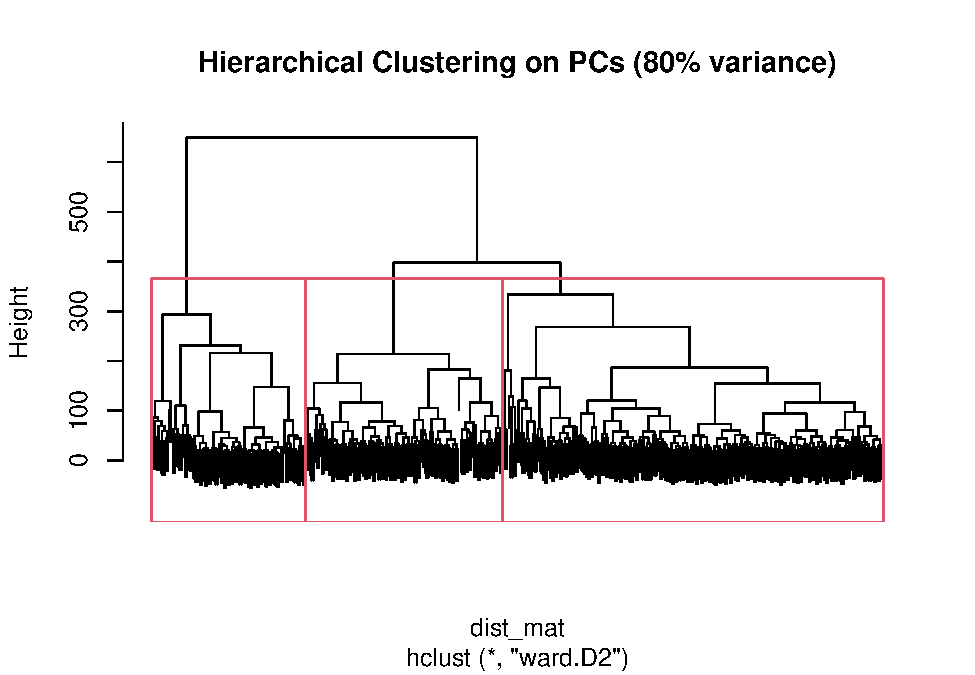
\includegraphics[keepaspectratio]{BMEG_310_Final_Project_P2_files/figure-latex/unnamed-chunk-14-1.pdf}}

\begin{Shaded}
\begin{Highlighting}[]
\FunctionTok{png}\NormalTok{(}\StringTok{"dendrogram.png"}\NormalTok{, }\AttributeTok{width =} \DecValTok{2400}\NormalTok{, }\AttributeTok{height =} \DecValTok{1800}\NormalTok{, }\AttributeTok{res =} \DecValTok{300}\NormalTok{)}
\FunctionTok{plot}\NormalTok{(hc, }\AttributeTok{labels =} \ConstantTok{FALSE}\NormalTok{, }\AttributeTok{main =} \StringTok{"Hierarchical Clustering on PCs (80\% variance)"}\NormalTok{)}
\FunctionTok{rect.hclust}\NormalTok{(hc, }\AttributeTok{k =} \DecValTok{3}\NormalTok{, }\AttributeTok{border =} \DecValTok{2}\NormalTok{)}
\FunctionTok{dev.off}\NormalTok{()}
\end{Highlighting}
\end{Shaded}

\begin{verbatim}
## pdf 
##   2
\end{verbatim}

\#Cutting Dendogram We decided to cut the dendrogram at 6 since there is
6 subtypes of KIRC

\begin{Shaded}
\begin{Highlighting}[]
\NormalTok{clusters }\OtherTok{\textless{}{-}} \FunctionTok{cutree}\NormalTok{(hc, }\AttributeTok{k =} \DecValTok{3}\NormalTok{)}
\FunctionTok{table}\NormalTok{(clusters)}
\end{Highlighting}
\end{Shaded}

\begin{verbatim}
## clusters
##   1   2   3 
## 222 115  90
\end{verbatim}

\section{Plot Overlapping Elbow and silhouette
graphs}\label{plot-overlapping-elbow-and-silhouette-graphs}

Do not pick 2, Since it was proven online that they might be artifacts
of batch effects

\begin{Shaded}
\begin{Highlighting}[]
\CommentTok{\# install.packages("factoextra")}
\FunctionTok{library}\NormalTok{(factoextra)}
\end{Highlighting}
\end{Shaded}

\begin{verbatim}
## Warning: package 'factoextra' was built under R version 4.5.2
\end{verbatim}

\begin{verbatim}
## Welcome! Want to learn more? See two factoextra-related books at https://goo.gl/ve3WBa
\end{verbatim}

\begin{Shaded}
\begin{Highlighting}[]
\CommentTok{\# Silhouette width }
\NormalTok{silhouette }\OtherTok{\textless{}{-}} \FunctionTok{fviz\_nbclust}\NormalTok{(}\FunctionTok{as.matrix}\NormalTok{(dist\_mat), hcut, }\AttributeTok{method =} \StringTok{"silhouette"}\NormalTok{, }\AttributeTok{hc\_method =} \StringTok{"ward.D2"}\NormalTok{)}
\NormalTok{silhouette}
\end{Highlighting}
\end{Shaded}

\pandocbounded{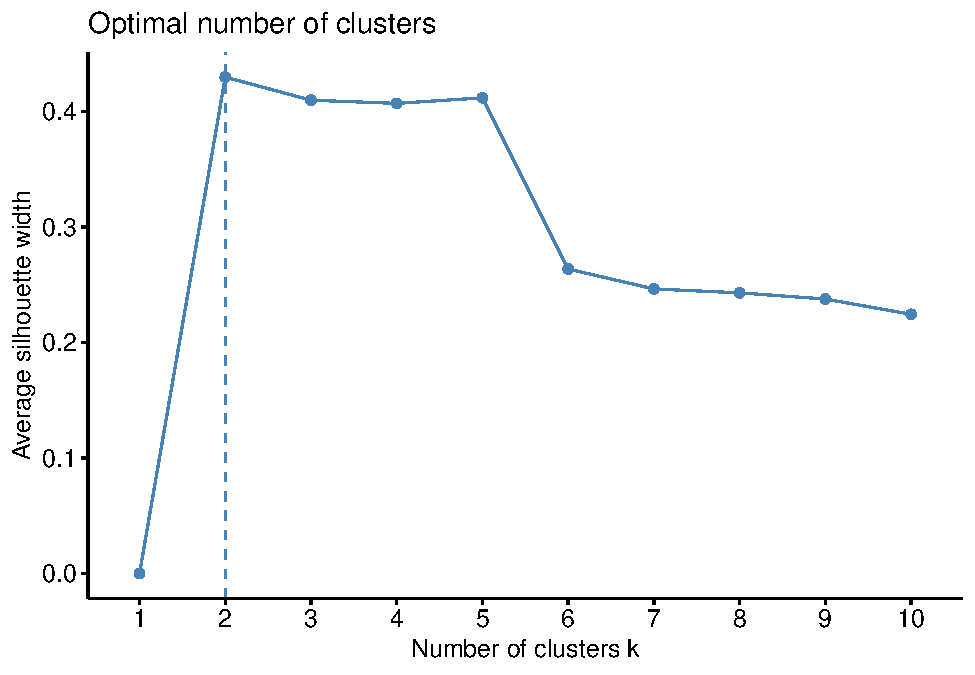
\includegraphics[keepaspectratio]{BMEG_310_Final_Project_P2_files/figure-latex/unnamed-chunk-16-1.pdf}}

\begin{Shaded}
\begin{Highlighting}[]
\CommentTok{\# Elbow plot}
\NormalTok{withinsumsquares }\OtherTok{\textless{}{-}} \FunctionTok{fviz\_nbclust}\NormalTok{(}\FunctionTok{as.matrix}\NormalTok{(dist\_mat), hcut, }\AttributeTok{method =} \StringTok{"wss"}\NormalTok{, }\AttributeTok{hc\_method =} \StringTok{"ward.D2"}\NormalTok{)}
\NormalTok{withinsumsquares}
\end{Highlighting}
\end{Shaded}

\pandocbounded{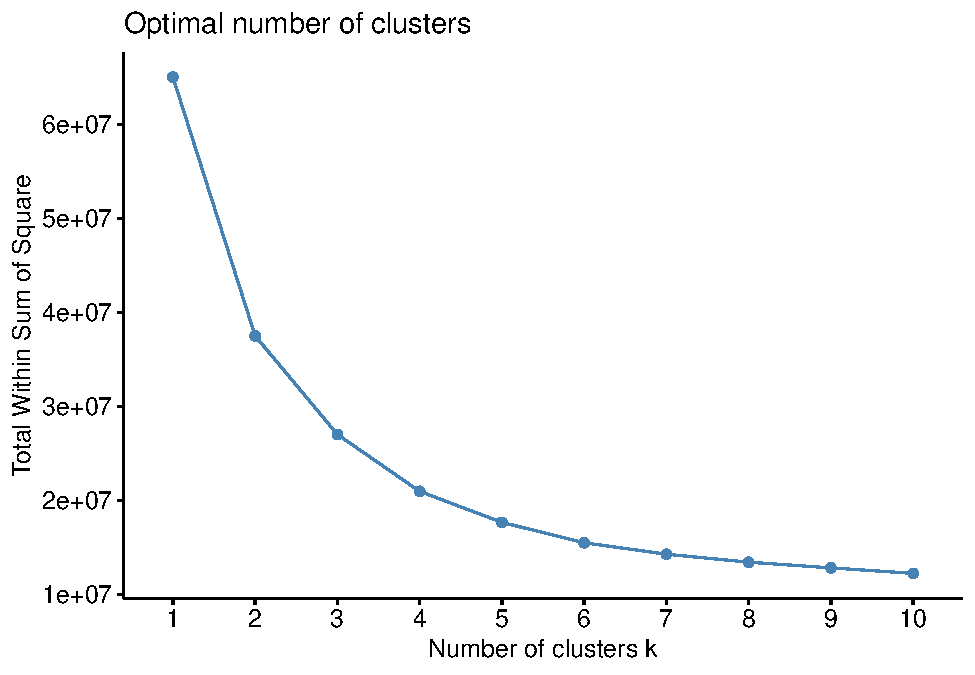
\includegraphics[keepaspectratio]{BMEG_310_Final_Project_P2_files/figure-latex/unnamed-chunk-16-2.pdf}}

\begin{Shaded}
\begin{Highlighting}[]
\FunctionTok{ggsave}\NormalTok{(}\StringTok{"silhouette\_plot.png"}\NormalTok{, silhouette, }\AttributeTok{width =} \DecValTok{7}\NormalTok{, }\AttributeTok{height =} \DecValTok{5}\NormalTok{, }\AttributeTok{dpi =} \DecValTok{300}\NormalTok{)}
\FunctionTok{ggsave}\NormalTok{(}\StringTok{"elbow\_plot.png"}\NormalTok{, withinsumsquares, }\AttributeTok{width =} \DecValTok{7}\NormalTok{, }\AttributeTok{height =} \DecValTok{5}\NormalTok{, }\AttributeTok{dpi =} \DecValTok{300}\NormalTok{)}
\end{Highlighting}
\end{Shaded}

\section{============================================================================}\label{section-9}

\section{INVESTIGATION 2: Survival across the patient clusters is
different.}\label{investigation-2-survival-across-the-patient-clusters-is-different.}

\section{RQ 2.2: Do expression-based clusters differ in patient
outcomes?}\label{rq-2.2-do-expression-based-clusters-differ-in-patient-outcomes}

\section{============================================================================}\label{section-10}

\section{Create a dataframe that contains the DSS and the cluster
labels. Rowname is patient
ID}\label{create-a-dataframe-that-contains-the-dss-and-the-cluster-labels.-rowname-is-patient-id}

\begin{Shaded}
\begin{Highlighting}[]
\CommentTok{\# Create a dataframe that contains the cluster and the patient ID}
\NormalTok{clustering\_data }\OtherTok{\textless{}{-}} \FunctionTok{data.frame}\NormalTok{(}
  \AttributeTok{clusters =}\NormalTok{ clusters,}
  \AttributeTok{PATIENT\_ID =} \FunctionTok{names}\NormalTok{(clusters)}
\NormalTok{)}

\CommentTok{\# transform clustering data into standard patient ID}
\NormalTok{clustering\_data}\SpecialCharTok{$}\NormalTok{PATIENT\_ID }\OtherTok{\textless{}{-}} \FunctionTok{gsub}\NormalTok{(}\StringTok{"}\SpecialCharTok{\textbackslash{}\textbackslash{}}\StringTok{."}\NormalTok{, }\StringTok{"{-}"}\NormalTok{, }\FunctionTok{substr}\NormalTok{(clustering\_data}\SpecialCharTok{$}\NormalTok{PATIENT\_ID, }\DecValTok{1}\NormalTok{, }\DecValTok{12}\NormalTok{))}

\FunctionTok{rownames}\NormalTok{(clustering\_data) }\OtherTok{\textless{}{-}} \ConstantTok{NULL}

\NormalTok{clinical\_data\_subset }\OtherTok{\textless{}{-}}\NormalTok{ data\_clinical\_patient[}
\NormalTok{ data\_clinical\_patient}\SpecialCharTok{$}\NormalTok{PATIENT\_ID }\SpecialCharTok{\%in\%}\NormalTok{ clustering\_data}\SpecialCharTok{$}\NormalTok{PATIENT\_ID,}
 \FunctionTok{c}\NormalTok{(}\StringTok{"PATIENT\_ID"}\NormalTok{, }\StringTok{"DSS\_STATUS"}\NormalTok{, }\StringTok{"DSS\_MONTHS"}\NormalTok{)}
\NormalTok{]}

\CommentTok{\# transform the DSS status to binary}
\NormalTok{clinical\_data\_subset}\SpecialCharTok{$}\NormalTok{DSS\_STATUS }\OtherTok{\textless{}{-}} \FunctionTok{substr}\NormalTok{(clinical\_data\_subset}\SpecialCharTok{$}\NormalTok{DSS\_STATUS, }\DecValTok{1}\NormalTok{, }\DecValTok{1}\NormalTok{)}

\NormalTok{merged\_data }\OtherTok{\textless{}{-}} \FunctionTok{merge}\NormalTok{(}
\NormalTok{ clustering\_data,}
\NormalTok{ clinical\_data\_subset,}
 \AttributeTok{by =} \StringTok{"PATIENT\_ID"}\NormalTok{,}
 \AttributeTok{all.x =} \ConstantTok{FALSE}\NormalTok{,}
 \AttributeTok{all.y =} \ConstantTok{FALSE}
\NormalTok{)}
\end{Highlighting}
\end{Shaded}

\section{Survival Analysis Across different
clusters}\label{survival-analysis-across-different-clusters}

\begin{Shaded}
\begin{Highlighting}[]
\NormalTok{surv\_obj\_ward\_DSS }\OtherTok{\textless{}{-}} \FunctionTok{Surv}\NormalTok{(}\AttributeTok{time =} \FunctionTok{as.numeric}\NormalTok{(merged\_data}\SpecialCharTok{$}\NormalTok{DSS\_MONTHS), }\AttributeTok{event=} \FunctionTok{as.numeric}\NormalTok{(merged\_data}\SpecialCharTok{$}\NormalTok{DSS\_STATUS))}

\CommentTok{\# KM plot for ward.D2 clustering}
\NormalTok{ward\_d2\_DSS }\OtherTok{\textless{}{-}} \FunctionTok{surv\_fit}\NormalTok{(surv\_obj\_ward\_DSS }\SpecialCharTok{\textasciitilde{}}\NormalTok{ clusters, }\AttributeTok{data =}\NormalTok{ merged\_data)}
\NormalTok{ward\_d2\_DSS\_plot }\OtherTok{\textless{}{-}} \FunctionTok{ggsurvplot}\NormalTok{(ward\_d2\_DSS,}
           \AttributeTok{data =}\NormalTok{ merged\_data,}
           \AttributeTok{pval =} \ConstantTok{TRUE}\NormalTok{,}
           \AttributeTok{conf.int =} \ConstantTok{TRUE}\NormalTok{,}
           \AttributeTok{title =} \StringTok{"Disease Specific Survival for Identified Ward.D2 Hierarchical Clusters"}\NormalTok{,}
           \AttributeTok{xlab =} \StringTok{"Time (Months)"}\NormalTok{,}
           \AttributeTok{ylab =} \StringTok{"Survival Probability"}\NormalTok{,}
           \AttributeTok{ggtheme =} \FunctionTok{theme\_minimal}\NormalTok{(}\AttributeTok{base\_size =} \DecValTok{14}\NormalTok{))}
\end{Highlighting}
\end{Shaded}

\begin{verbatim}
## Warning: Using `size` aesthetic for lines was deprecated in ggplot2 3.4.0.
## i Please use `linewidth` instead.
## i The deprecated feature was likely used in the ggpubr package.
##   Please report the issue at <https://github.com/kassambara/ggpubr/issues>.
## This warning is displayed once every 8 hours.
## Call `lifecycle::last_lifecycle_warnings()` to see where this warning was
## generated.
\end{verbatim}

\begin{Shaded}
\begin{Highlighting}[]
\NormalTok{ward\_d2\_DSS\_plot}
\end{Highlighting}
\end{Shaded}

\pandocbounded{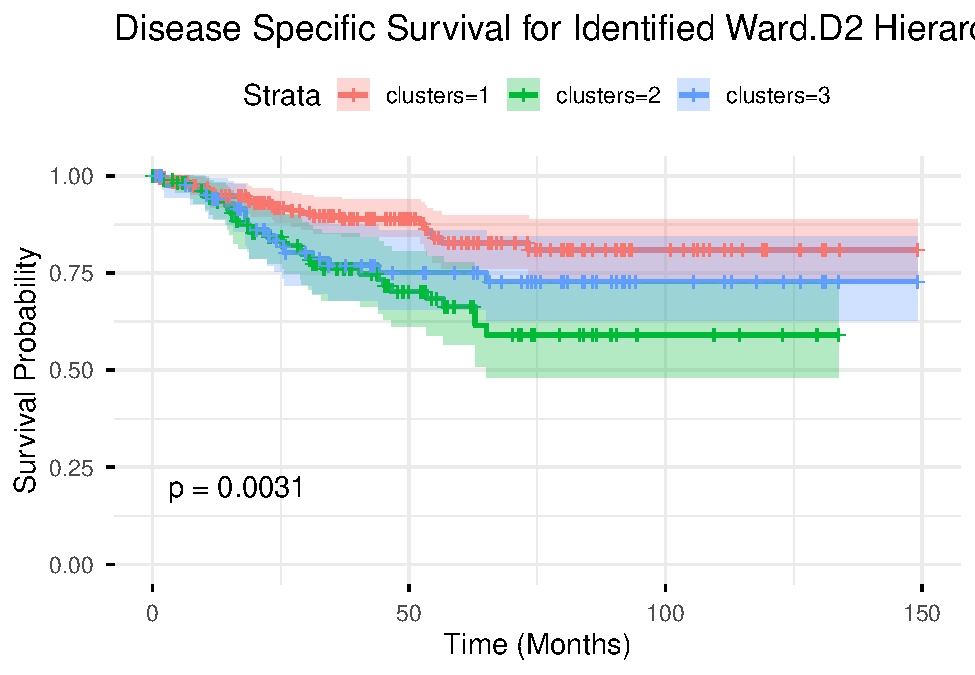
\includegraphics[keepaspectratio]{BMEG_310_Final_Project_P2_files/figure-latex/unnamed-chunk-18-1.pdf}}

\begin{Shaded}
\begin{Highlighting}[]
\FunctionTok{ggsave}\NormalTok{(}\StringTok{"DSSacrossclusters.png"}\NormalTok{, ward\_d2\_DSS\_plot}\SpecialCharTok{$}\NormalTok{plot, }\AttributeTok{width=}\DecValTok{7}\NormalTok{, }\AttributeTok{height=}\DecValTok{3}\NormalTok{, }\AttributeTok{dpi=}\DecValTok{300}\NormalTok{)}
\end{Highlighting}
\end{Shaded}

Since we see 3 clear outcomes in survival. This is good since there is 3
histological subtypes

\section{Assign the clusters to respective patients and their
data}\label{assign-the-clusters-to-respective-patients-and-their-data}

\begin{Shaded}
\begin{Highlighting}[]
\CommentTok{\# Create a dataframe that contains the cluster and the patient ID}
\NormalTok{clustering\_data }\OtherTok{\textless{}{-}} \FunctionTok{data.frame}\NormalTok{(}
  \AttributeTok{clusters =}\NormalTok{ clusters,}
  \AttributeTok{PATIENT\_ID =} \FunctionTok{names}\NormalTok{(clusters)}
\NormalTok{)}

\CommentTok{\# Transform clustering data into standard patient ID}
\NormalTok{clustering\_data}\SpecialCharTok{$}\NormalTok{PATIENT\_ID }\OtherTok{\textless{}{-}} \FunctionTok{gsub}\NormalTok{(}\StringTok{"}\SpecialCharTok{\textbackslash{}\textbackslash{}}\StringTok{."}\NormalTok{, }\StringTok{"{-}"}\NormalTok{, }\FunctionTok{substr}\NormalTok{(clustering\_data}\SpecialCharTok{$}\NormalTok{PATIENT\_ID, }\DecValTok{1}\NormalTok{, }\DecValTok{12}\NormalTok{))}
\FunctionTok{rownames}\NormalTok{(clustering\_data) }\OtherTok{\textless{}{-}} \ConstantTok{NULL}

\CommentTok{\# Extract relevant clinical data}
\NormalTok{clinical\_data\_subset }\OtherTok{\textless{}{-}}\NormalTok{ data\_clinical\_patient[}
\NormalTok{  data\_clinical\_patient}\SpecialCharTok{$}\NormalTok{PATIENT\_ID }\SpecialCharTok{\%in\%}\NormalTok{ clustering\_data}\SpecialCharTok{$}\NormalTok{PATIENT\_ID,}
  \FunctionTok{c}\NormalTok{(}\StringTok{"PATIENT\_ID"}\NormalTok{, }\StringTok{"DSS\_STATUS"}\NormalTok{, }\StringTok{"DSS\_MONTHS"}\NormalTok{, }\StringTok{"AGE"}\NormalTok{, }\StringTok{"AJCC\_PATHOLOGIC\_TUMOR\_STAGE"}\NormalTok{)}
\NormalTok{]}

\CommentTok{\# Transform the DSS status to binary (0 = alive, 1 = dead)}
\NormalTok{clinical\_data\_subset}\SpecialCharTok{$}\NormalTok{DSS\_STATUS }\OtherTok{\textless{}{-}} \FunctionTok{substr}\NormalTok{(clinical\_data\_subset}\SpecialCharTok{$}\NormalTok{DSS\_STATUS, }\DecValTok{1}\NormalTok{, }\DecValTok{1}\NormalTok{)}

\CommentTok{\# Transform the tumor stage}
\NormalTok{clinical\_data\_subset}\SpecialCharTok{$}\NormalTok{AJCC\_PATHOLOGIC\_TUMOR\_STAGE }\OtherTok{\textless{}{-}} \FunctionTok{sapply}\NormalTok{(clinical\_data\_subset}\SpecialCharTok{$}\NormalTok{AJCC\_PATHOLOGIC\_TUMOR\_STAGE, }\ControlFlowTok{function}\NormalTok{(x) \{}
  \ControlFlowTok{if}\NormalTok{ (}\FunctionTok{grepl}\NormalTok{(}\StringTok{"stage"}\NormalTok{, x, }\AttributeTok{ignore.case =} \ConstantTok{TRUE}\NormalTok{)) \{}
            \FunctionTok{as.numeric}\NormalTok{(}\FunctionTok{as.roman}\NormalTok{(}\FunctionTok{gsub}\NormalTok{(}\StringTok{"stage "}\NormalTok{, }\StringTok{""}\NormalTok{, x, }\AttributeTok{ignore.case =} \ConstantTok{TRUE}\NormalTok{)))}
\NormalTok{  \} }\ControlFlowTok{else}\NormalTok{ \{}
    \ConstantTok{NA}  
\NormalTok{  \}}
\NormalTok{\})}

\CommentTok{\# Merge clustering and clinical data}
\NormalTok{merged\_data }\OtherTok{\textless{}{-}} \FunctionTok{merge}\NormalTok{(}
\NormalTok{  clustering\_data,}
\NormalTok{  clinical\_data\_subset,}
  \AttributeTok{by =} \StringTok{"PATIENT\_ID"}\NormalTok{,}
  \AttributeTok{all.x =} \ConstantTok{FALSE}\NormalTok{,}
  \AttributeTok{all.y =} \ConstantTok{FALSE}
\NormalTok{)}
\end{Highlighting}
\end{Shaded}

\section{Look for diffences in age - ANOVA. Code adapted from part 1 of
the
project.}\label{look-for-diffences-in-age---anova.-code-adapted-from-part-1-of-the-project.}

\begin{Shaded}
\begin{Highlighting}[]
\CommentTok{\# One{-}way ANOVA for age}
\NormalTok{merged\_data}\SpecialCharTok{$}\NormalTok{clusters }\OtherTok{\textless{}{-}} \FunctionTok{as.factor}\NormalTok{(merged\_data}\SpecialCharTok{$}\NormalTok{clusters)}

\NormalTok{anova\_result\_Ward\_D2 }\OtherTok{\textless{}{-}} \FunctionTok{aov}\NormalTok{(merged\_data}\SpecialCharTok{$}\NormalTok{AGE }\SpecialCharTok{\textasciitilde{}}\NormalTok{ clusters, }\AttributeTok{data =}\NormalTok{ merged\_data)}
\FunctionTok{summary}\NormalTok{(anova\_result\_Ward\_D2)}
\end{Highlighting}
\end{Shaded}

\begin{verbatim}
##              Df Sum Sq Mean Sq F value Pr(>F)
## clusters      2     32   16.24   0.114  0.893
## Residuals   424  60571  142.86
\end{verbatim}

\begin{Shaded}
\begin{Highlighting}[]
\FunctionTok{TukeyHSD}\NormalTok{(anova\_result\_Ward\_D2)}
\end{Highlighting}
\end{Shaded}

\begin{verbatim}
##   Tukey multiple comparisons of means
##     95% family-wise confidence level
## 
## Fit: aov(formula = merged_data$AGE ~ clusters, data = merged_data)
## 
## $clusters
##           diff       lwr      upr     p adj
## 2-1  0.6336467 -2.596115 3.863409 0.8893148
## 3-1  0.3867868 -3.126071 3.899644 0.9637093
## 3-2 -0.2468599 -4.203146 3.709427 0.9881970
\end{verbatim}

\begin{Shaded}
\begin{Highlighting}[]
\NormalTok{anova\_ward\_d2\_plot }\OtherTok{\textless{}{-}} \FunctionTok{ggplot}\NormalTok{(merged\_data, }\FunctionTok{aes}\NormalTok{(}\AttributeTok{x =}\NormalTok{ clusters, }\AttributeTok{y =}\NormalTok{ AGE, }\AttributeTok{fill =}\NormalTok{ clusters)) }\SpecialCharTok{+}
  \FunctionTok{geom\_boxplot}\NormalTok{() }\SpecialCharTok{+}
  \FunctionTok{labs}\NormalTok{(}
    \AttributeTok{title =} \StringTok{"Patient Age Distribution Across Ward.D2 Clusters"}\NormalTok{,}
    \AttributeTok{x =} \StringTok{"Cluster"}\NormalTok{,}
    \AttributeTok{y =} \StringTok{"Age (years)"}
\NormalTok{  ) }\SpecialCharTok{+}
  \FunctionTok{theme\_minimal}\NormalTok{(}\AttributeTok{base\_size =} \DecValTok{14}\NormalTok{) }\SpecialCharTok{+}
  \FunctionTok{theme}\NormalTok{(}\AttributeTok{legend.position =} \StringTok{"none"}\NormalTok{)}

\CommentTok{\# Plot}
\NormalTok{anova\_ward\_d2\_plot}
\end{Highlighting}
\end{Shaded}

\pandocbounded{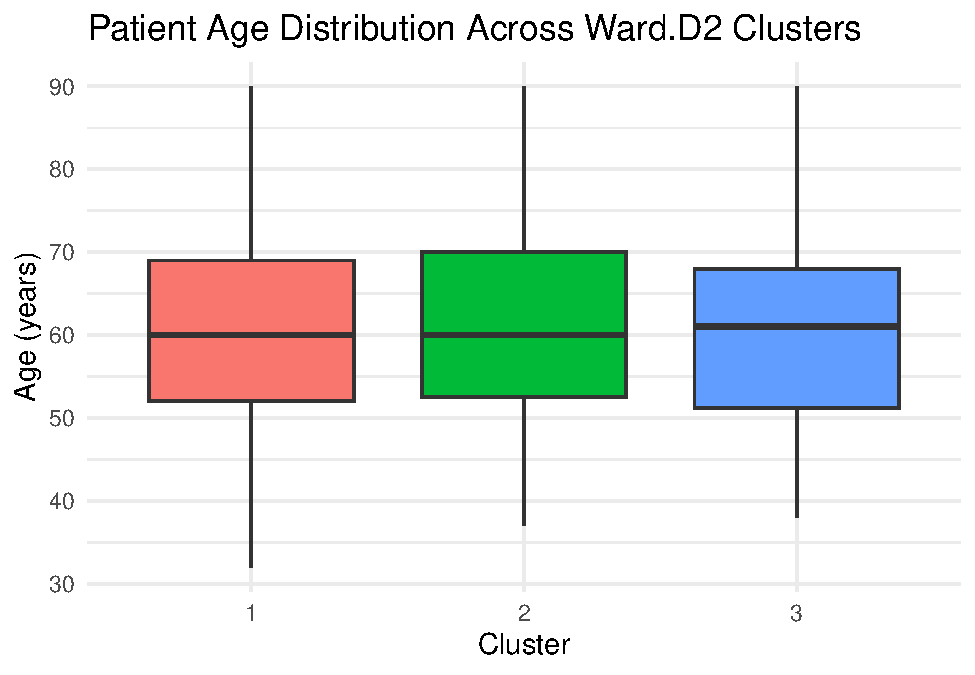
\includegraphics[keepaspectratio]{BMEG_310_Final_Project_P2_files/figure-latex/unnamed-chunk-20-1.pdf}}

\begin{Shaded}
\begin{Highlighting}[]
\FunctionTok{ggsave}\NormalTok{(}\StringTok{"AgeDistributionAcrossClusters\_WardD2.png"}\NormalTok{, anova\_ward\_d2\_plot, }\AttributeTok{width=}\DecValTok{7}\NormalTok{, }\AttributeTok{height=}\DecValTok{3}\NormalTok{, }\AttributeTok{dpi=}\DecValTok{300}\NormalTok{)}
\end{Highlighting}
\end{Shaded}

\section{What about Tumor stage?}\label{what-about-tumor-stage}

\begin{Shaded}
\begin{Highlighting}[]
\NormalTok{merged\_data}\SpecialCharTok{$}\NormalTok{AJCC\_PATHOLOGIC\_TUMOR\_STAGE }\OtherTok{\textless{}{-}} \FunctionTok{as.factor}\NormalTok{(merged\_data}\SpecialCharTok{$}\NormalTok{AJCC\_PATHOLOGIC\_TUMOR\_STAGE)}

\CommentTok{\# Contingency table}
\NormalTok{table\_stage\_cluster\_wardd2 }\OtherTok{\textless{}{-}} \FunctionTok{table}\NormalTok{(merged\_data}\SpecialCharTok{$}\NormalTok{clusters, merged\_data}\SpecialCharTok{$}\NormalTok{AJCC\_PATHOLOGIC\_TUMOR\_STAGE)}
\NormalTok{table\_stage\_cluster\_wardd2}
\end{Highlighting}
\end{Shaded}

\begin{verbatim}
##    
##       1   2   3   4
##   1 126  24  47  25
##   2  46  13  33  23
##   3  39  16  15  20
\end{verbatim}

\begin{Shaded}
\begin{Highlighting}[]
\CommentTok{\# Chi{-}square Test}
\NormalTok{chisq\_test\_wardd2 }\OtherTok{\textless{}{-}} \FunctionTok{chisq.test}\NormalTok{(table\_stage\_cluster\_wardd2)}
\NormalTok{chisq\_test\_wardd2}
\end{Highlighting}
\end{Shaded}

\begin{verbatim}
## 
##  Pearson's Chi-squared test
## 
## data:  table_stage_cluster_wardd2
## X-squared = 17.815, df = 6, p-value = 0.006711
\end{verbatim}

\begin{Shaded}
\begin{Highlighting}[]
\CommentTok{\# Visualization}
\NormalTok{chi\_test\_plot\_ward2 }\OtherTok{\textless{}{-}} \FunctionTok{ggplot}\NormalTok{(merged\_data, }\FunctionTok{aes}\NormalTok{(}\AttributeTok{x =}\NormalTok{ clusters, }\AttributeTok{fill =}\NormalTok{ AJCC\_PATHOLOGIC\_TUMOR\_STAGE)) }\SpecialCharTok{+}
  \FunctionTok{geom\_bar}\NormalTok{(}\AttributeTok{position =} \StringTok{"fill"}\NormalTok{) }\SpecialCharTok{+}  \CommentTok{\# fill = proportion per cluster}
  \FunctionTok{coord\_flip}\NormalTok{() }\SpecialCharTok{+}
  \FunctionTok{ylab}\NormalTok{(}\StringTok{"Proportion"}\NormalTok{) }\SpecialCharTok{+}
  \FunctionTok{xlab}\NormalTok{(}\StringTok{"Cluster"}\NormalTok{) }\SpecialCharTok{+}
  \FunctionTok{labs}\NormalTok{(}\AttributeTok{title =} \StringTok{"Tumor Stage Across Ward.D2 Clusters"}\NormalTok{, }\AttributeTok{fill =} \StringTok{"Tumor Stage"}\NormalTok{) }\SpecialCharTok{+}
  \FunctionTok{theme\_minimal}\NormalTok{(}\AttributeTok{base\_size =} \DecValTok{14}\NormalTok{)}

\CommentTok{\#plot}
\NormalTok{chi\_test\_plot\_ward2}
\end{Highlighting}
\end{Shaded}

\pandocbounded{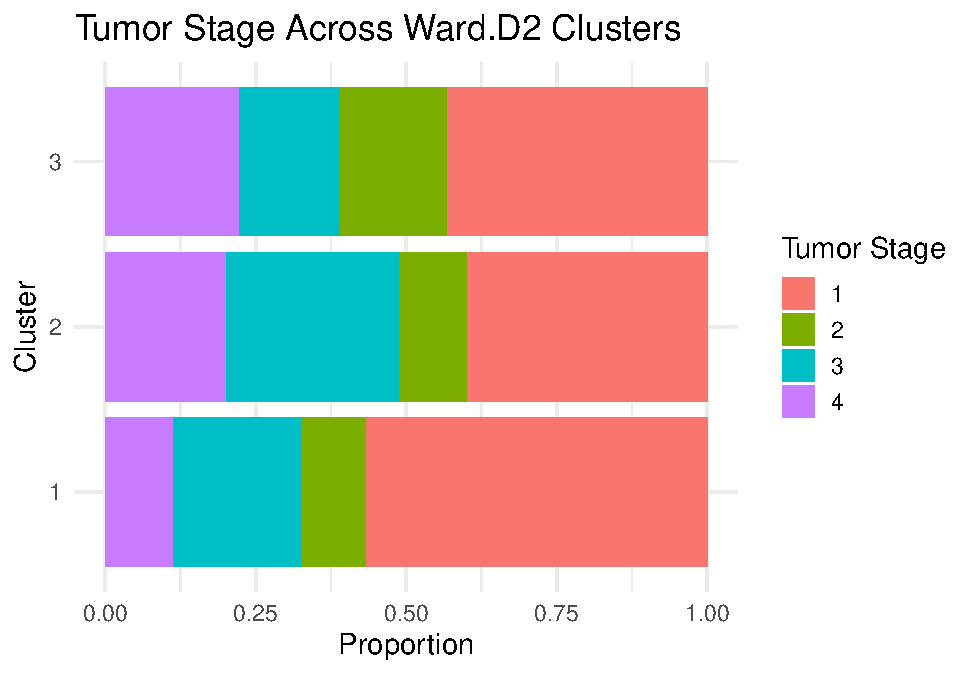
\includegraphics[keepaspectratio]{BMEG_310_Final_Project_P2_files/figure-latex/unnamed-chunk-21-1.pdf}}

\begin{Shaded}
\begin{Highlighting}[]
\CommentTok{\#save}
\FunctionTok{ggsave}\NormalTok{(}\StringTok{"TumorStageAcrossClusters\_WardD2.png"}\NormalTok{,chi\_test\_plot\_ward2 , }\AttributeTok{width=}\DecValTok{7}\NormalTok{, }\AttributeTok{height=}\DecValTok{3}\NormalTok{, }\AttributeTok{dpi=}\DecValTok{300}\NormalTok{)}
\end{Highlighting}
\end{Shaded}

\section{============================================================================}\label{section-11}

\section{INVESTIGATION 3: Check DE across
clusters}\label{investigation-3-check-de-across-clusters}

\section{RQ 2.2: What gene vary across clusters? Are they Significative
of KIRC
subtype?}\label{rq-2.2-what-gene-vary-across-clusters-are-they-significative-of-kirc-subtype}

\section{============================================================================}\label{section-12}

\section{============================================================================}\label{section-13}

\section{Run DESeq2 for Differential Expression Between
Clusters}\label{run-deseq2-for-differential-expression-between-clusters}

\section{============================================================================}\label{section-14}

This step was made by claudeAI usign the prompt(s):``Read this +
Previous code, and make a DE heatmap using pheatmap''

\begin{Shaded}
\begin{Highlighting}[]
\FunctionTok{cat}\NormalTok{(}\StringTok{"Merged data dimensions:"}\NormalTok{, }\FunctionTok{dim}\NormalTok{(merged\_data), }\StringTok{"}\SpecialCharTok{\textbackslash{}n}\StringTok{"}\NormalTok{)}
\end{Highlighting}
\end{Shaded}

\begin{verbatim}
## Merged data dimensions: 427 6
\end{verbatim}

\begin{Shaded}
\begin{Highlighting}[]
\FunctionTok{cat}\NormalTok{(}\StringTok{"Cluster distribution:}\SpecialCharTok{\textbackslash{}n}\StringTok{"}\NormalTok{)}
\end{Highlighting}
\end{Shaded}

\begin{verbatim}
## Cluster distribution:
\end{verbatim}

\begin{Shaded}
\begin{Highlighting}[]
\FunctionTok{print}\NormalTok{(}\FunctionTok{table}\NormalTok{(merged\_data}\SpecialCharTok{$}\NormalTok{clusters))}
\end{Highlighting}
\end{Shaded}

\begin{verbatim}
## 
##   1   2   3 
## 222 115  90
\end{verbatim}

\begin{Shaded}
\begin{Highlighting}[]
\FunctionTok{cat}\NormalTok{(}\StringTok{"}\SpecialCharTok{\textbackslash{}n}\StringTok{"}\NormalTok{)}
\end{Highlighting}
\end{Shaded}

\begin{Shaded}
\begin{Highlighting}[]
\CommentTok{\# ============================================================================}
\CommentTok{\# Run DESeq2 for Differential Expression Between Clusters}
\CommentTok{\# ============================================================================}

\CommentTok{\# Prepare DESeq2 object with cluster information}
\CommentTok{\# Use the original sample names (with dots/full barcodes)}
\NormalTok{coldata\_clusters }\OtherTok{\textless{}{-}} \FunctionTok{data.frame}\NormalTok{(}
  \AttributeTok{sample =} \FunctionTok{colnames}\NormalTok{(count\_matrix),}
  \AttributeTok{cluster =}\NormalTok{ clusters[}\FunctionTok{colnames}\NormalTok{(count\_matrix)]}
\NormalTok{)}
\FunctionTok{rownames}\NormalTok{(coldata\_clusters) }\OtherTok{\textless{}{-}}\NormalTok{ coldata\_clusters}\SpecialCharTok{$}\NormalTok{sample}
\NormalTok{coldata\_clusters}\SpecialCharTok{$}\NormalTok{cluster }\OtherTok{\textless{}{-}} \FunctionTok{as.factor}\NormalTok{(coldata\_clusters}\SpecialCharTok{$}\NormalTok{cluster)}

\CommentTok{\# Create DESeq2 dataset with cluster design}
\NormalTok{dds\_de }\OtherTok{\textless{}{-}} \FunctionTok{DESeqDataSetFromMatrix}\NormalTok{(}
  \AttributeTok{countData =}\NormalTok{ count\_matrix,}
  \AttributeTok{colData =}\NormalTok{ coldata\_clusters,}
  \AttributeTok{design =} \SpecialCharTok{\textasciitilde{}}\NormalTok{ cluster}
\NormalTok{)}

\CommentTok{\# Filter low{-}count genes (at least 10 reads in at least 10\% of samples)}
\NormalTok{keep }\OtherTok{\textless{}{-}} \FunctionTok{rowSums}\NormalTok{(}\FunctionTok{counts}\NormalTok{(dds\_de) }\SpecialCharTok{\textgreater{}=} \DecValTok{10}\NormalTok{) }\SpecialCharTok{\textgreater{}=} \FunctionTok{ncol}\NormalTok{(dds\_de) }\SpecialCharTok{*} \FloatTok{0.1}
\NormalTok{dds\_de }\OtherTok{\textless{}{-}}\NormalTok{ dds\_de[keep, ]}
\FunctionTok{cat}\NormalTok{(}\StringTok{"Genes retained after filtering:"}\NormalTok{, }\FunctionTok{nrow}\NormalTok{(dds\_de), }\StringTok{"}\SpecialCharTok{\textbackslash{}n\textbackslash{}n}\StringTok{"}\NormalTok{)}
\end{Highlighting}
\end{Shaded}

\begin{verbatim}
## Genes retained after filtering: 26443
\end{verbatim}

\begin{Shaded}
\begin{Highlighting}[]
\CommentTok{\# Run DESeq2}
\NormalTok{dds\_de }\OtherTok{\textless{}{-}} \FunctionTok{DESeq}\NormalTok{(dds\_de)}
\end{Highlighting}
\end{Shaded}

\begin{verbatim}
## estimating size factors
\end{verbatim}

\begin{verbatim}
## estimating dispersions
\end{verbatim}

\begin{verbatim}
## gene-wise dispersion estimates
\end{verbatim}

\begin{verbatim}
## mean-dispersion relationship
\end{verbatim}

\begin{verbatim}
## final dispersion estimates
\end{verbatim}

\begin{verbatim}
## fitting model and testing
\end{verbatim}

\begin{verbatim}
## -- replacing outliers and refitting for 2237 genes
## -- DESeq argument 'minReplicatesForReplace' = 7 
## -- original counts are preserved in counts(dds)
\end{verbatim}

\begin{verbatim}
## estimating dispersions
\end{verbatim}

\begin{verbatim}
## fitting model and testing
\end{verbatim}

\begin{Shaded}
\begin{Highlighting}[]
\CommentTok{\# ============================================================================}
\CommentTok{\# Extract Top Differentially Expressed Genes}
\CommentTok{\# ============================================================================}

\CommentTok{\# Get all pairwise comparisons}
\NormalTok{comparisons }\OtherTok{\textless{}{-}} \FunctionTok{list}\NormalTok{(}
  \AttributeTok{c1\_vs\_c2 =} \FunctionTok{results}\NormalTok{(dds\_de, }\AttributeTok{contrast =} \FunctionTok{c}\NormalTok{(}\StringTok{"cluster"}\NormalTok{, }\StringTok{"1"}\NormalTok{, }\StringTok{"2"}\NormalTok{)),}
  \AttributeTok{c1\_vs\_c3 =} \FunctionTok{results}\NormalTok{(dds\_de, }\AttributeTok{contrast =} \FunctionTok{c}\NormalTok{(}\StringTok{"cluster"}\NormalTok{, }\StringTok{"1"}\NormalTok{, }\StringTok{"3"}\NormalTok{)),}
  \AttributeTok{c2\_vs\_c3 =} \FunctionTok{results}\NormalTok{(dds\_de, }\AttributeTok{contrast =} \FunctionTok{c}\NormalTok{(}\StringTok{"cluster"}\NormalTok{, }\StringTok{"2"}\NormalTok{, }\StringTok{"3"}\NormalTok{))}
\NormalTok{)}

\CommentTok{\# Find significant DEGs for each comparison (padj \textless{} 0.05, |log2FC| \textgreater{} 1)}
\NormalTok{sig\_genes\_list }\OtherTok{\textless{}{-}} \FunctionTok{lapply}\NormalTok{(comparisons, }\ControlFlowTok{function}\NormalTok{(res) \{}
\NormalTok{  sig }\OtherTok{\textless{}{-}}\NormalTok{ res[}\FunctionTok{which}\NormalTok{(res}\SpecialCharTok{$}\NormalTok{padj }\SpecialCharTok{\textless{}} \FloatTok{0.05} \SpecialCharTok{\&} \FunctionTok{abs}\NormalTok{(res}\SpecialCharTok{$}\NormalTok{log2FoldChange) }\SpecialCharTok{\textgreater{}} \DecValTok{1}\NormalTok{), ]}
  \FunctionTok{rownames}\NormalTok{(sig)}
\NormalTok{\})}

\CommentTok{\# Combine all significant genes}
\NormalTok{all\_sig\_genes }\OtherTok{\textless{}{-}} \FunctionTok{unique}\NormalTok{(}\FunctionTok{unlist}\NormalTok{(sig\_genes\_list))}
\FunctionTok{cat}\NormalTok{(}\StringTok{"Total unique DEGs across all comparisons:"}\NormalTok{, }\FunctionTok{length}\NormalTok{(all\_sig\_genes), }\StringTok{"}\SpecialCharTok{\textbackslash{}n}\StringTok{"}\NormalTok{)}
\end{Highlighting}
\end{Shaded}

\begin{verbatim}
## Total unique DEGs across all comparisons: 11683
\end{verbatim}

\begin{Shaded}
\begin{Highlighting}[]
\CommentTok{\# Select top genes by variance if there are too many}
\ControlFlowTok{if}\NormalTok{ (}\FunctionTok{length}\NormalTok{(all\_sig\_genes) }\SpecialCharTok{\textgreater{}} \DecValTok{500}\NormalTok{) \{}
\NormalTok{  gene\_vars\_sig }\OtherTok{\textless{}{-}} \FunctionTok{apply}\NormalTok{(vst\_counts[all\_sig\_genes, ], }\DecValTok{1}\NormalTok{, var)}
\NormalTok{  top\_sig\_genes }\OtherTok{\textless{}{-}} \FunctionTok{names}\NormalTok{(}\FunctionTok{sort}\NormalTok{(gene\_vars\_sig, }\AttributeTok{decreasing =} \ConstantTok{TRUE}\NormalTok{))[}\DecValTok{1}\SpecialCharTok{:}\DecValTok{500}\NormalTok{]}
  \FunctionTok{cat}\NormalTok{(}\StringTok{"Selected top 500 DEGs by variance}\SpecialCharTok{\textbackslash{}n\textbackslash{}n}\StringTok{"}\NormalTok{)}
\NormalTok{\} }\ControlFlowTok{else}\NormalTok{ \{}
\NormalTok{  top\_sig\_genes }\OtherTok{\textless{}{-}}\NormalTok{ all\_sig\_genes}
\NormalTok{\}}
\end{Highlighting}
\end{Shaded}

\begin{verbatim}
## Selected top 500 DEGs by variance
\end{verbatim}

\section{Create Heatmap}\label{create-heatmap}

\begin{Shaded}
\begin{Highlighting}[]
\CommentTok{\# Extract VST counts for top DEGs}
\NormalTok{heatmap\_data }\OtherTok{\textless{}{-}}\NormalTok{ vst\_counts[top\_sig\_genes, ]}

\CommentTok{\# Z{-}score normalize by gene (rows)}
\NormalTok{heatmap\_data\_scaled }\OtherTok{\textless{}{-}} \FunctionTok{t}\NormalTok{(}\FunctionTok{scale}\NormalTok{(}\FunctionTok{t}\NormalTok{(heatmap\_data)))}

\CommentTok{\# Order samples by cluster}
\NormalTok{sample\_order }\OtherTok{\textless{}{-}} \FunctionTok{order}\NormalTok{(clusters)}
\NormalTok{heatmap\_data\_scaled }\OtherTok{\textless{}{-}}\NormalTok{ heatmap\_data\_scaled[, sample\_order]}
\NormalTok{clusters\_ordered }\OtherTok{\textless{}{-}}\NormalTok{ clusters[sample\_order]}

\CommentTok{\# Create annotation for samples (columns)}
\NormalTok{annotation\_col }\OtherTok{\textless{}{-}} \FunctionTok{data.frame}\NormalTok{(}
  \AttributeTok{Cluster =} \FunctionTok{as.factor}\NormalTok{(clusters\_ordered)}
\NormalTok{)}
\FunctionTok{rownames}\NormalTok{(annotation\_col) }\OtherTok{\textless{}{-}} \FunctionTok{colnames}\NormalTok{(heatmap\_data\_scaled)}

\CommentTok{\# Define colors for clusters}
\NormalTok{cluster\_colors }\OtherTok{\textless{}{-}} \FunctionTok{list}\NormalTok{(}
  \AttributeTok{Cluster =} \FunctionTok{c}\NormalTok{(}\StringTok{"1"} \OtherTok{=} \StringTok{"\#E69F00"}\NormalTok{, }\StringTok{"2"} \OtherTok{=} \StringTok{"\#56B4E9"}\NormalTok{, }\StringTok{"3"} \OtherTok{=} \StringTok{"\#009E73"}\NormalTok{)}
\NormalTok{)}
\end{Highlighting}
\end{Shaded}

\section{Save the image}\label{save-the-image}

\begin{Shaded}
\begin{Highlighting}[]
\CommentTok{\# Create the heatmap}
\NormalTok{DEheatmap }\OtherTok{\textless{}{-}} \FunctionTok{pheatmap}\NormalTok{(}
\NormalTok{  heatmap\_data\_scaled,}
  \AttributeTok{scale =} \StringTok{"none"}\NormalTok{,  }\CommentTok{\# Already scaled}
  \AttributeTok{cluster\_rows =} \ConstantTok{TRUE}\NormalTok{,  }\CommentTok{\# Cluster genes}
  \AttributeTok{cluster\_cols =} \ConstantTok{FALSE}\NormalTok{,  }\CommentTok{\# Keep sample order by cluster}
  \AttributeTok{clustering\_distance\_rows =} \StringTok{"euclidean"}\NormalTok{,}
  \AttributeTok{clustering\_method =} \StringTok{"ward.D2"}\NormalTok{,}
  \AttributeTok{annotation\_col =}\NormalTok{ annotation\_col,}
  \AttributeTok{annotation\_colors =}\NormalTok{ cluster\_colors,}
  \AttributeTok{show\_colnames =} \ConstantTok{FALSE}\NormalTok{,  }\CommentTok{\# Too many samples}
  \AttributeTok{show\_rownames =} \ConstantTok{FALSE}\NormalTok{,  }\CommentTok{\# Too many genes}
  \AttributeTok{color =} \FunctionTok{colorRampPalette}\NormalTok{(}\FunctionTok{c}\NormalTok{(}\StringTok{"green"}\NormalTok{, }\StringTok{"black"}\NormalTok{, }\StringTok{"red"}\NormalTok{))(}\DecValTok{100}\NormalTok{),}
  \AttributeTok{main =} \StringTok{"Differential Gene Expression Across Clusters"}\NormalTok{,}
  \AttributeTok{fontsize =} \DecValTok{10}\NormalTok{,}
  \AttributeTok{border\_color =} \ConstantTok{NA}\NormalTok{,}
  \CommentTok{\#filename = "DEpercluster.png"  \# Add this parameter}
\NormalTok{)}
\end{Highlighting}
\end{Shaded}

\pandocbounded{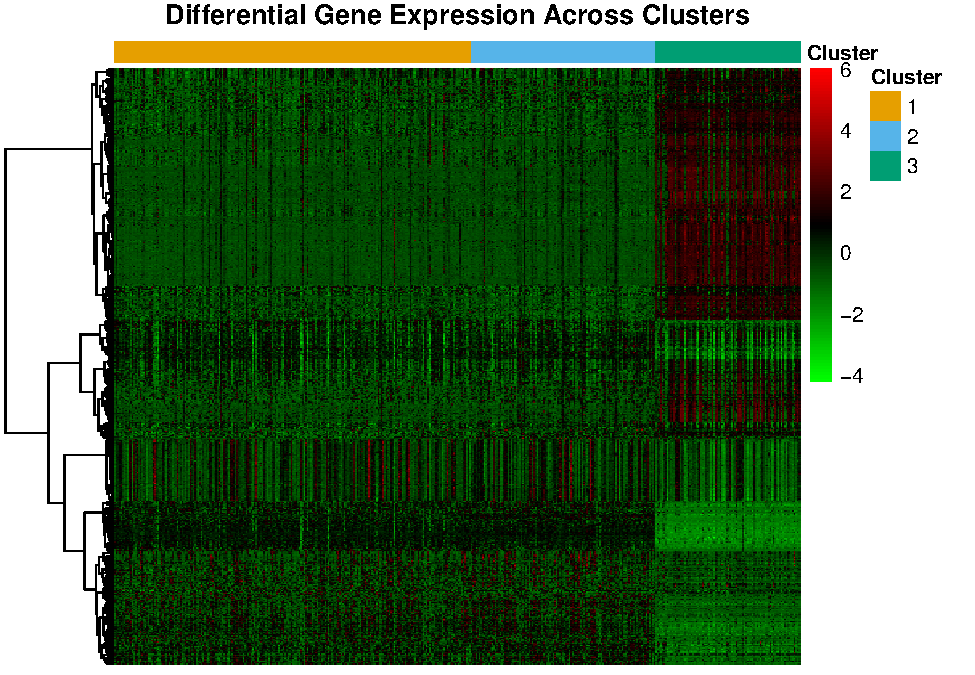
\includegraphics[keepaspectratio]{BMEG_310_Final_Project_P2_files/figure-latex/unnamed-chunk-24-1.pdf}}
\# Which genes are the most differentially expressed? Code belwo was
generated with ClaudeAI and the prompts: I want as simple as possible,
in R so I can see hte comparisons. + Code aboe

\begin{Shaded}
\begin{Highlighting}[]
\FunctionTok{library}\NormalTok{(ggplot2)}
\FunctionTok{library}\NormalTok{(gridExtra)}
\end{Highlighting}
\end{Shaded}

\begin{verbatim}
## 
## Attaching package: 'gridExtra'
\end{verbatim}

\begin{verbatim}
## The following object is masked from 'package:dplyr':
## 
##     combine
\end{verbatim}

\begin{verbatim}
## The following object is masked from 'package:Biobase':
## 
##     combine
\end{verbatim}

\begin{verbatim}
## The following object is masked from 'package:BiocGenerics':
## 
##     combine
\end{verbatim}

\begin{Shaded}
\begin{Highlighting}[]
\CommentTok{\# Function to create volcano plot}
\NormalTok{make\_volcano }\OtherTok{\textless{}{-}} \ControlFlowTok{function}\NormalTok{(res, title) \{}
  \CommentTok{\# Prepare data}
\NormalTok{  df }\OtherTok{\textless{}{-}} \FunctionTok{as.data.frame}\NormalTok{(res)}
\NormalTok{  df}\SpecialCharTok{$}\NormalTok{gene }\OtherTok{\textless{}{-}} \FunctionTok{rownames}\NormalTok{(df)}
\NormalTok{  df}\SpecialCharTok{$}\NormalTok{neglog10padj }\OtherTok{\textless{}{-}} \SpecialCharTok{{-}}\FunctionTok{log10}\NormalTok{(df}\SpecialCharTok{$}\NormalTok{padj)}
  
  \CommentTok{\# Add significance category}
\NormalTok{  df}\SpecialCharTok{$}\NormalTok{significance }\OtherTok{\textless{}{-}} \StringTok{"Not Significant"}
\NormalTok{  df}\SpecialCharTok{$}\NormalTok{significance[df}\SpecialCharTok{$}\NormalTok{padj }\SpecialCharTok{\textless{}} \FloatTok{0.05} \SpecialCharTok{\&}\NormalTok{ df}\SpecialCharTok{$}\NormalTok{log2FoldChange }\SpecialCharTok{\textgreater{}} \DecValTok{1}\NormalTok{] }\OtherTok{\textless{}{-}} \StringTok{"Upregulated"}
\NormalTok{  df}\SpecialCharTok{$}\NormalTok{significance[df}\SpecialCharTok{$}\NormalTok{padj }\SpecialCharTok{\textless{}} \FloatTok{0.05} \SpecialCharTok{\&}\NormalTok{ df}\SpecialCharTok{$}\NormalTok{log2FoldChange }\SpecialCharTok{\textless{}} \SpecialCharTok{{-}}\DecValTok{1}\NormalTok{] }\OtherTok{\textless{}{-}} \StringTok{"Downregulated"}
\NormalTok{  df}\SpecialCharTok{$}\NormalTok{significance }\OtherTok{\textless{}{-}} \FunctionTok{factor}\NormalTok{(df}\SpecialCharTok{$}\NormalTok{significance, }
                           \AttributeTok{levels =} \FunctionTok{c}\NormalTok{(}\StringTok{"Upregulated"}\NormalTok{, }\StringTok{"Downregulated"}\NormalTok{, }\StringTok{"Not Significant"}\NormalTok{))}
  
  \CommentTok{\# Remove NA values}
\NormalTok{  df }\OtherTok{\textless{}{-}}\NormalTok{ df[}\SpecialCharTok{!}\FunctionTok{is.na}\NormalTok{(df}\SpecialCharTok{$}\NormalTok{padj) }\SpecialCharTok{\&} \SpecialCharTok{!}\FunctionTok{is.na}\NormalTok{(df}\SpecialCharTok{$}\NormalTok{log2FoldChange), ]}
  
  \CommentTok{\# Count genes in each category}
\NormalTok{  n\_up }\OtherTok{\textless{}{-}} \FunctionTok{sum}\NormalTok{(df}\SpecialCharTok{$}\NormalTok{significance }\SpecialCharTok{==} \StringTok{"Upregulated"}\NormalTok{)}
\NormalTok{  n\_down }\OtherTok{\textless{}{-}} \FunctionTok{sum}\NormalTok{(df}\SpecialCharTok{$}\NormalTok{significance }\SpecialCharTok{==} \StringTok{"Downregulated"}\NormalTok{)}
  
  \CommentTok{\# Create plot}
\NormalTok{  p }\OtherTok{\textless{}{-}} \FunctionTok{ggplot}\NormalTok{(df, }\FunctionTok{aes}\NormalTok{(}\AttributeTok{x =}\NormalTok{ log2FoldChange, }\AttributeTok{y =}\NormalTok{ neglog10padj, }\AttributeTok{color =}\NormalTok{ significance)) }\SpecialCharTok{+}
    \FunctionTok{geom\_point}\NormalTok{(}\AttributeTok{alpha =} \FloatTok{0.6}\NormalTok{, }\AttributeTok{size =} \FloatTok{1.5}\NormalTok{) }\SpecialCharTok{+}
    \FunctionTok{scale\_color\_manual}\NormalTok{(}\AttributeTok{values =} \FunctionTok{c}\NormalTok{(}\StringTok{"Upregulated"} \OtherTok{=} \StringTok{"\#ef4444"}\NormalTok{, }
                                  \StringTok{"Downregulated"} \OtherTok{=} \StringTok{"\#3b82f6"}\NormalTok{, }
                                  \StringTok{"Not Significant"} \OtherTok{=} \StringTok{"\#9ca3af"}\NormalTok{)) }\SpecialCharTok{+}
    \FunctionTok{geom\_vline}\NormalTok{(}\AttributeTok{xintercept =} \FunctionTok{c}\NormalTok{(}\SpecialCharTok{{-}}\DecValTok{1}\NormalTok{, }\DecValTok{1}\NormalTok{), }\AttributeTok{linetype =} \StringTok{"dashed"}\NormalTok{, }\AttributeTok{color =} \StringTok{"gray50"}\NormalTok{) }\SpecialCharTok{+}
    \FunctionTok{geom\_hline}\NormalTok{(}\AttributeTok{yintercept =} \SpecialCharTok{{-}}\FunctionTok{log10}\NormalTok{(}\FloatTok{0.05}\NormalTok{), }\AttributeTok{linetype =} \StringTok{"dashed"}\NormalTok{, }\AttributeTok{color =} \StringTok{"gray50"}\NormalTok{) }\SpecialCharTok{+}
    \FunctionTok{labs}\NormalTok{(}\AttributeTok{title =}\NormalTok{ title,}
         \AttributeTok{subtitle =} \FunctionTok{paste0}\NormalTok{(}\StringTok{"Up: "}\NormalTok{, n\_up, }\StringTok{" | Down: "}\NormalTok{, n\_down),}
         \AttributeTok{x =} \StringTok{"log2 Fold Change"}\NormalTok{,}
         \AttributeTok{y =} \StringTok{"{-}log10(adjusted p{-}value)"}\NormalTok{,}
         \AttributeTok{color =} \StringTok{"Significance"}\NormalTok{) }\SpecialCharTok{+}
    \FunctionTok{theme\_bw}\NormalTok{() }\SpecialCharTok{+}
    \FunctionTok{theme}\NormalTok{(}\AttributeTok{plot.title =} \FunctionTok{element\_text}\NormalTok{(}\AttributeTok{hjust =} \FloatTok{0.5}\NormalTok{, }\AttributeTok{face =} \StringTok{"bold"}\NormalTok{),}
          \AttributeTok{plot.subtitle =} \FunctionTok{element\_text}\NormalTok{(}\AttributeTok{hjust =} \FloatTok{0.5}\NormalTok{),}
          \AttributeTok{legend.position =} \StringTok{"bottom"}\NormalTok{)}
  
  \FunctionTok{return}\NormalTok{(p)}
\NormalTok{\}}

\CommentTok{\# Create volcano plots for each comparison}
\NormalTok{p1 }\OtherTok{\textless{}{-}} \FunctionTok{make\_volcano}\NormalTok{(comparisons}\SpecialCharTok{$}\NormalTok{c1\_vs\_c2, }\StringTok{"Cluster 1 vs Cluster 2"}\NormalTok{)}
\NormalTok{p2 }\OtherTok{\textless{}{-}} \FunctionTok{make\_volcano}\NormalTok{(comparisons}\SpecialCharTok{$}\NormalTok{c1\_vs\_c3, }\StringTok{"Cluster 1 vs Cluster 3"}\NormalTok{)}
\NormalTok{p3 }\OtherTok{\textless{}{-}} \FunctionTok{make\_volcano}\NormalTok{(comparisons}\SpecialCharTok{$}\NormalTok{c2\_vs\_c3, }\StringTok{"Cluster 2 vs Cluster 3"}\NormalTok{)}

\CommentTok{\# Display all three plots}
\FunctionTok{grid.arrange}\NormalTok{(p1, p2, p3, }\AttributeTok{ncol =} \DecValTok{3}\NormalTok{)}
\end{Highlighting}
\end{Shaded}

\pandocbounded{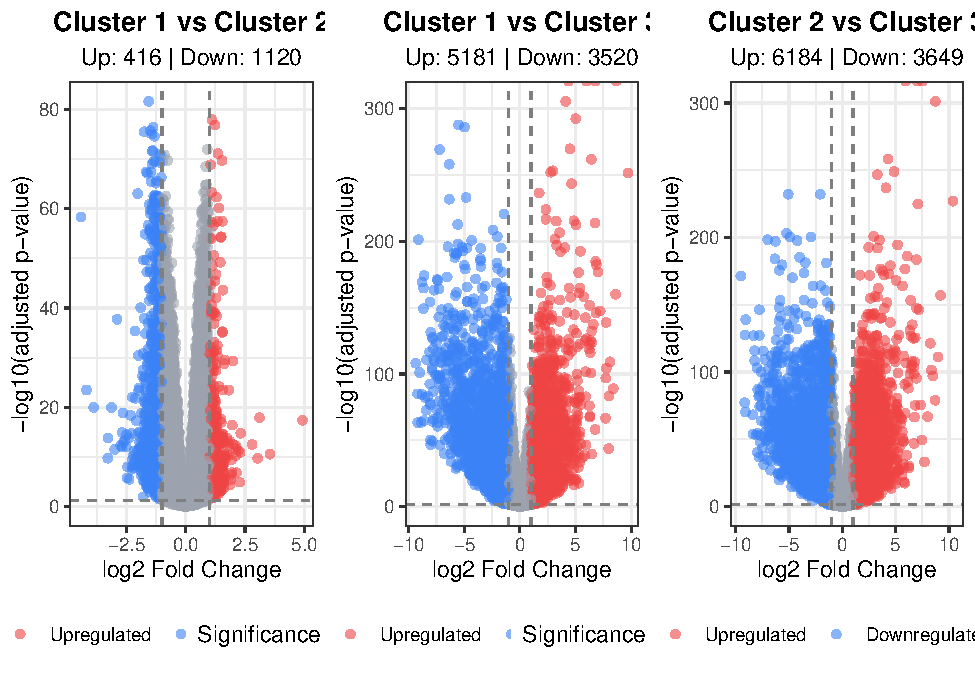
\includegraphics[keepaspectratio]{BMEG_310_Final_Project_P2_files/figure-latex/unnamed-chunk-25-1.pdf}}

\begin{Shaded}
\begin{Highlighting}[]
\CommentTok{\# Optional: Save as high{-}resolution figure}
\FunctionTok{ggsave}\NormalTok{(}\StringTok{"volcano\_c1\_vs\_c2.png"}\NormalTok{, p1, }\AttributeTok{width =} \DecValTok{8}\NormalTok{, }\AttributeTok{height =} \DecValTok{6}\NormalTok{, }\AttributeTok{dpi =} \DecValTok{300}\NormalTok{)}
\FunctionTok{ggsave}\NormalTok{(}\StringTok{"volcano\_c1\_vs\_c3.png"}\NormalTok{, p2, }\AttributeTok{width =} \DecValTok{8}\NormalTok{, }\AttributeTok{height =} \DecValTok{6}\NormalTok{, }\AttributeTok{dpi =} \DecValTok{300}\NormalTok{)}
\FunctionTok{ggsave}\NormalTok{(}\StringTok{"volcano\_c2\_vs\_c3.png"}\NormalTok{, p3, }\AttributeTok{width =} \DecValTok{8}\NormalTok{, }\AttributeTok{height =} \DecValTok{6}\NormalTok{, }\AttributeTok{dpi =} \DecValTok{300}\NormalTok{)}
\end{Highlighting}
\end{Shaded}

\section{Which genes (by name) are the most differentially
expressed?}\label{which-genes-by-name-are-the-most-differentially-expressed}

\begin{Shaded}
\begin{Highlighting}[]
\FunctionTok{cat}\NormalTok{(}\StringTok{"}\SpecialCharTok{\textbackslash{}n}\StringTok{=== Differential Expression Summary ===}\SpecialCharTok{\textbackslash{}n}\StringTok{"}\NormalTok{)}
\end{Highlighting}
\end{Shaded}

\begin{verbatim}
## 
## === Differential Expression Summary ===
\end{verbatim}

\begin{Shaded}
\begin{Highlighting}[]
\ControlFlowTok{for}\NormalTok{(comp\_name }\ControlFlowTok{in} \FunctionTok{names}\NormalTok{(comparisons)) \{}
\NormalTok{  res }\OtherTok{\textless{}{-}}\NormalTok{ comparisons[[comp\_name]]}
\NormalTok{  df }\OtherTok{\textless{}{-}} \FunctionTok{as.data.frame}\NormalTok{(res)}
\NormalTok{  df}\SpecialCharTok{$}\NormalTok{gene }\OtherTok{\textless{}{-}} \FunctionTok{rownames}\NormalTok{(df)}
\NormalTok{  df }\OtherTok{\textless{}{-}}\NormalTok{ df[}\SpecialCharTok{!}\FunctionTok{is.na}\NormalTok{(df}\SpecialCharTok{$}\NormalTok{padj), ]}
  
\NormalTok{  n\_up }\OtherTok{\textless{}{-}} \FunctionTok{sum}\NormalTok{(df}\SpecialCharTok{$}\NormalTok{padj }\SpecialCharTok{\textless{}} \FloatTok{0.05} \SpecialCharTok{\&}\NormalTok{ df}\SpecialCharTok{$}\NormalTok{log2FoldChange }\SpecialCharTok{\textgreater{}} \DecValTok{1}\NormalTok{, }\AttributeTok{na.rm =} \ConstantTok{TRUE}\NormalTok{)}
\NormalTok{  n\_down }\OtherTok{\textless{}{-}} \FunctionTok{sum}\NormalTok{(df}\SpecialCharTok{$}\NormalTok{padj }\SpecialCharTok{\textless{}} \FloatTok{0.05} \SpecialCharTok{\&}\NormalTok{ df}\SpecialCharTok{$}\NormalTok{log2FoldChange }\SpecialCharTok{\textless{}} \SpecialCharTok{{-}}\DecValTok{1}\NormalTok{, }\AttributeTok{na.rm =} \ConstantTok{TRUE}\NormalTok{)}
\NormalTok{  n\_total\_sig }\OtherTok{\textless{}{-}} \FunctionTok{sum}\NormalTok{(df}\SpecialCharTok{$}\NormalTok{padj }\SpecialCharTok{\textless{}} \FloatTok{0.05}\NormalTok{, }\AttributeTok{na.rm =} \ConstantTok{TRUE}\NormalTok{)}
  
  \FunctionTok{cat}\NormalTok{(}\FunctionTok{sprintf}\NormalTok{(}\StringTok{"}\SpecialCharTok{\textbackslash{}n}\StringTok{\%s:}\SpecialCharTok{\textbackslash{}n}\StringTok{"}\NormalTok{, comp\_name))}
  \FunctionTok{cat}\NormalTok{(}\FunctionTok{sprintf}\NormalTok{(}\StringTok{"  Upregulated (padj\textless{}0.05, log2FC\textgreater{}1): \%d}\SpecialCharTok{\textbackslash{}n}\StringTok{"}\NormalTok{, n\_up))}
  \FunctionTok{cat}\NormalTok{(}\FunctionTok{sprintf}\NormalTok{(}\StringTok{"  Downregulated (padj\textless{}0.05, log2FC\textless{}{-}1): \%d}\SpecialCharTok{\textbackslash{}n}\StringTok{"}\NormalTok{, n\_down))}
  \FunctionTok{cat}\NormalTok{(}\FunctionTok{sprintf}\NormalTok{(}\StringTok{"  Total significant (padj\textless{}0.05): \%d}\SpecialCharTok{\textbackslash{}n}\StringTok{"}\NormalTok{, n\_total\_sig))}
  
  \CommentTok{\# Get top upregulated genes}
  \FunctionTok{cat}\NormalTok{(}\StringTok{"}\SpecialCharTok{\textbackslash{}n}\StringTok{  Top 10 UPREGULATED genes:}\SpecialCharTok{\textbackslash{}n}\StringTok{"}\NormalTok{)}
\NormalTok{  top\_up }\OtherTok{\textless{}{-}}\NormalTok{ df[df}\SpecialCharTok{$}\NormalTok{padj }\SpecialCharTok{\textless{}} \FloatTok{0.05} \SpecialCharTok{\&}\NormalTok{ df}\SpecialCharTok{$}\NormalTok{log2FoldChange }\SpecialCharTok{\textgreater{}} \DecValTok{0}\NormalTok{, ]}
\NormalTok{  top\_up }\OtherTok{\textless{}{-}}\NormalTok{ top\_up[}\FunctionTok{order}\NormalTok{(top\_up}\SpecialCharTok{$}\NormalTok{log2FoldChange, }\AttributeTok{decreasing =} \ConstantTok{TRUE}\NormalTok{), ]}
  \ControlFlowTok{if}\NormalTok{(}\FunctionTok{nrow}\NormalTok{(top\_up) }\SpecialCharTok{\textgreater{}} \DecValTok{0}\NormalTok{) \{}
    \ControlFlowTok{for}\NormalTok{(i }\ControlFlowTok{in} \DecValTok{1}\SpecialCharTok{:}\FunctionTok{min}\NormalTok{(}\DecValTok{10}\NormalTok{, }\FunctionTok{nrow}\NormalTok{(top\_up))) \{}
      \FunctionTok{cat}\NormalTok{(}\FunctionTok{sprintf}\NormalTok{(}\StringTok{"    \%2d. \%{-}15s | log2FC: \%6.2f | padj: \%.2e}\SpecialCharTok{\textbackslash{}n}\StringTok{"}\NormalTok{, }
\NormalTok{                  i, top\_up}\SpecialCharTok{$}\NormalTok{gene[i], top\_up}\SpecialCharTok{$}\NormalTok{log2FoldChange[i], top\_up}\SpecialCharTok{$}\NormalTok{padj[i]))}
\NormalTok{    \}}
\NormalTok{  \} }\ControlFlowTok{else}\NormalTok{ \{}
    \FunctionTok{cat}\NormalTok{(}\StringTok{"    No significantly upregulated genes}\SpecialCharTok{\textbackslash{}n}\StringTok{"}\NormalTok{)}
\NormalTok{  \}}
  
  \CommentTok{\# Get top downregulated genes}
  \FunctionTok{cat}\NormalTok{(}\StringTok{"}\SpecialCharTok{\textbackslash{}n}\StringTok{  Top 10 DOWNREGULATED genes:}\SpecialCharTok{\textbackslash{}n}\StringTok{"}\NormalTok{)}
\NormalTok{  top\_down }\OtherTok{\textless{}{-}}\NormalTok{ df[df}\SpecialCharTok{$}\NormalTok{padj }\SpecialCharTok{\textless{}} \FloatTok{0.05} \SpecialCharTok{\&}\NormalTok{ df}\SpecialCharTok{$}\NormalTok{log2FoldChange }\SpecialCharTok{\textless{}} \DecValTok{0}\NormalTok{, ]}
\NormalTok{  top\_down }\OtherTok{\textless{}{-}}\NormalTok{ top\_down[}\FunctionTok{order}\NormalTok{(top\_down}\SpecialCharTok{$}\NormalTok{log2FoldChange, }\AttributeTok{decreasing =} \ConstantTok{FALSE}\NormalTok{), ]}
  \ControlFlowTok{if}\NormalTok{(}\FunctionTok{nrow}\NormalTok{(top\_down) }\SpecialCharTok{\textgreater{}} \DecValTok{0}\NormalTok{) \{}
    \ControlFlowTok{for}\NormalTok{(i }\ControlFlowTok{in} \DecValTok{1}\SpecialCharTok{:}\FunctionTok{min}\NormalTok{(}\DecValTok{10}\NormalTok{, }\FunctionTok{nrow}\NormalTok{(top\_down))) \{}
      \FunctionTok{cat}\NormalTok{(}\FunctionTok{sprintf}\NormalTok{(}\StringTok{"    \%2d. \%{-}15s | log2FC: \%6.2f | padj: \%.2e}\SpecialCharTok{\textbackslash{}n}\StringTok{"}\NormalTok{, }
\NormalTok{                  i, top\_down}\SpecialCharTok{$}\NormalTok{gene[i], top\_down}\SpecialCharTok{$}\NormalTok{log2FoldChange[i], top\_down}\SpecialCharTok{$}\NormalTok{padj[i]))}
\NormalTok{    \}}
\NormalTok{  \} }\ControlFlowTok{else}\NormalTok{ \{}
    \FunctionTok{cat}\NormalTok{(}\StringTok{"    No significantly downregulated genes}\SpecialCharTok{\textbackslash{}n}\StringTok{"}\NormalTok{)}
\NormalTok{  \}}
  \FunctionTok{cat}\NormalTok{(}\StringTok{"}\SpecialCharTok{\textbackslash{}n}\StringTok{"}\NormalTok{, }\FunctionTok{strrep}\NormalTok{(}\StringTok{"{-}"}\NormalTok{, }\DecValTok{70}\NormalTok{), }\StringTok{"}\SpecialCharTok{\textbackslash{}n}\StringTok{"}\NormalTok{)}
\NormalTok{\}}
\end{Highlighting}
\end{Shaded}

\begin{verbatim}
## 
## c1_vs_c2:
##   Upregulated (padj<0.05, log2FC>1): 416
##   Downregulated (padj<0.05, log2FC<-1): 1120
##   Total significant (padj<0.05): 17275
## 
##   Top 10 UPREGULATED genes:
##      1. ENSG00000105141.6 | log2FC:   4.93 | padj: 4.23e-18
##      2. ENSG00000263146.2 | log2FC:   3.55 | padj: 2.91e-11
##      3. ENSG00000070915.10 | log2FC:   3.11 | padj: 1.27e-18
##      4. ENSG00000256463.8 | log2FC:   3.04 | padj: 1.90e-10
##      5. ENSG00000271945.2 | log2FC:   2.80 | padj: 3.06e-13
##      6. ENSG00000134258.17 | log2FC:   2.32 | padj: 1.81e-15
##      7. ENSG00000168143.9 | log2FC:   2.29 | padj: 1.26e-11
##      8. ENSG00000181092.10 | log2FC:   2.27 | padj: 1.16e-05
##      9. ENSG00000130294.17 | log2FC:   2.22 | padj: 5.78e-12
##     10. ENSG00000287702.1 | log2FC:   2.14 | padj: 1.49e-07
## 
##   Top 10 DOWNREGULATED genes:
##      1. ENSG00000225972.1 | log2FC:  -4.43 | padj: 5.35e-59
##      2. ENSG00000150201.15 | log2FC:  -4.19 | padj: 3.35e-24
##      3. ENSG00000223783.1 | log2FC:  -3.89 | padj: 1.12e-20
##      4. ENSG00000261667.1 | log2FC:  -3.29 | padj: 1.80e-10
##      5. ENSG00000253802.2 | log2FC:  -3.27 | padj: 1.52e-14
##      6. ENSG00000170367.5 | log2FC:  -3.13 | padj: 1.13e-20
##      7. ENSG00000254475.1 | log2FC:  -3.00 | padj: 3.09e-12
##      8. ENSG00000262902.1 | log2FC:  -2.90 | padj: 2.02e-38
##      9. ENSG00000261514.1 | log2FC:  -2.74 | padj: 5.23e-13
##     10. ENSG00000287407.1 | log2FC:  -2.70 | padj: 9.38e-13
## 
##  ---------------------------------------------------------------------- 
## 
## c1_vs_c3:
##   Upregulated (padj<0.05, log2FC>1): 5181
##   Downregulated (padj<0.05, log2FC<-1): 3520
##   Total significant (padj<0.05): 21326
## 
##   Top 10 UPREGULATED genes:
##      1. ENSG00000164434.12 | log2FC:   9.72 | padj: 4.41e-252
##      2. ENSG00000224490.5 | log2FC:   8.66 | padj: 0.00e+00
##      3. ENSG00000225174.2 | log2FC:   8.60 | padj: 8.93e-161
##      4. ENSG00000286085.1 | log2FC:   8.40 | padj: 1.33e-89
##      5. ENSG00000168619.16 | log2FC:   8.09 | padj: 6.90e-110
##      6. ENSG00000168333.14 | log2FC:   8.01 | padj: 5.88e-84
##      7. ENSG00000214978.7 | log2FC:   7.99 | padj: 1.92e-44
##      8. ENSG00000251320.1 | log2FC:   7.78 | padj: 4.23e-105
##      9. ENSG00000178776.5 | log2FC:   7.75 | padj: 1.96e-139
##     10. ENSG00000248362.1 | log2FC:   7.71 | padj: 1.40e-97
## 
##   Top 10 DOWNREGULATED genes:
##      1. ENSG00000174562.13 | log2FC:  -9.36 | padj: 8.83e-109
##      2. ENSG00000279460.1 | log2FC:  -9.19 | padj: 1.03e-85
##      3. ENSG00000169344.15 | log2FC:  -9.19 | padj: 4.35e-64
##      4. ENSG00000086159.13 | log2FC:  -9.12 | padj: 6.17e-202
##      5. ENSG00000225064.1 | log2FC:  -9.00 | padj: 9.46e-102
##      6. ENSG00000167580.8 | log2FC:  -8.89 | padj: 4.17e-64
##      7. ENSG00000168269.10 | log2FC:  -8.81 | padj: 2.65e-85
##      8. ENSG00000188175.10 | log2FC:  -8.81 | padj: 4.57e-170
##      9. ENSG00000249601.2 | log2FC:  -8.68 | padj: 7.01e-150
##     10. ENSG00000140519.14 | log2FC:  -8.66 | padj: 1.94e-165
## 
##  ---------------------------------------------------------------------- 
## 
## c2_vs_c3:
##   Upregulated (padj<0.05, log2FC>1): 6184
##   Downregulated (padj<0.05, log2FC<-1): 3649
##   Total significant (padj<0.05): 21766
## 
##   Top 10 UPREGULATED genes:
##      1. ENSG00000164434.12 | log2FC:  10.38 | padj: 1.32e-227
##      2. ENSG00000178776.5 | log2FC:   9.21 | padj: 1.13e-157
##      3. ENSG00000248362.1 | log2FC:   8.97 | padj: 5.95e-112
##      4. ENSG00000224490.5 | log2FC:   8.73 | padj: 7.90e-302
##      5. ENSG00000168333.14 | log2FC:   8.71 | padj: 1.02e-79
##      6. ENSG00000188373.5 | log2FC:   8.49 | padj: 9.54e-98
##      7. ENSG00000251320.1 | log2FC:   8.36 | padj: 3.34e-102
##      8. ENSG00000225174.2 | log2FC:   8.26 | padj: 4.38e-122
##      9. ENSG00000286085.1 | log2FC:   8.00 | padj: 1.65e-67
##     10. ENSG00000214978.7 | log2FC:   7.70 | padj: 6.26e-34
## 
##   Top 10 DOWNREGULATED genes:
##      1. ENSG00000086159.13 | log2FC:  -9.51 | padj: 3.93e-172
##      2. ENSG00000225064.1 | log2FC:  -9.15 | padj: 6.42e-78
##      3. ENSG00000249601.2 | log2FC:  -9.11 | padj: 2.85e-128
##      4. ENSG00000168269.10 | log2FC:  -9.06 | padj: 5.24e-71
##      5. ENSG00000188175.10 | log2FC:  -9.05 | padj: 9.72e-140
##      6. ENSG00000174562.13 | log2FC:  -8.39 | padj: 5.90e-69
##      7. ENSG00000173612.10 | log2FC:  -8.36 | padj: 9.60e-55
##      8. ENSG00000167748.11 | log2FC:  -8.29 | padj: 9.25e-128
##      9. ENSG00000105929.16 | log2FC:  -8.21 | padj: 1.46e-116
##     10. ENSG00000265460.6 | log2FC:  -8.20 | padj: 3.49e-109
## 
##  ----------------------------------------------------------------------
\end{verbatim}

\section{============================================================================}\label{section-15}

\section{INVESTIGATION 4:}\label{investigation-4}

\section{RQ 2.4:}\label{rq-2.4}

\section{============================================================================}\label{section-16}

\begin{Shaded}
\begin{Highlighting}[]
\DocumentationTok{\#\# Get Initial Count Matrix}
\CommentTok{\# Create count matrix (genes as rows, samples as columns)}
\NormalTok{count\_matrix }\OtherTok{\textless{}{-}} \FunctionTok{as.matrix}\NormalTok{(RNAseq\_KIRC[, }\SpecialCharTok{{-}}\DecValTok{1}\NormalTok{])  }\CommentTok{\# Remove gene name column}
\CommentTok{\# Assuming your Ensembl IDs are in the first column of RNAseq\_KIRC}
\NormalTok{ensemble\_ids }\OtherTok{\textless{}{-}}\NormalTok{ RNAseq\_KIRC[, }\DecValTok{1}\NormalTok{]}
\CommentTok{\# Fix common Ensembl ID format issue (remove version number like ".1")}
\CommentTok{\# This ensures a better match rate with the annotation package}
\NormalTok{ensemble\_ids\_clean }\OtherTok{\textless{}{-}} \FunctionTok{sub}\NormalTok{(}\StringTok{"}\SpecialCharTok{\textbackslash{}\textbackslash{}}\StringTok{.}\SpecialCharTok{\textbackslash{}\textbackslash{}}\StringTok{d+$"}\NormalTok{, }\StringTok{""}\NormalTok{, ensemble\_ids)}
\FunctionTok{rownames}\NormalTok{(count\_matrix) }\OtherTok{\textless{}{-}}\NormalTok{ ensemble\_ids\_clean}

\FunctionTok{cat}\NormalTok{(}\StringTok{"Initial count matrix dimensions (by Ensembl ID):"}\NormalTok{, }\FunctionTok{dim}\NormalTok{(count\_matrix), }\StringTok{"}\SpecialCharTok{\textbackslash{}n}\StringTok{"}\NormalTok{)}
\end{Highlighting}
\end{Shaded}

\begin{verbatim}
## Initial count matrix dimensions (by Ensembl ID): 60660 427
\end{verbatim}

\begin{Shaded}
\begin{Highlighting}[]
\CommentTok{\# Map Ensembl IDs to Gene Symbols}
\NormalTok{gene\_map }\OtherTok{\textless{}{-}} \FunctionTok{select}\NormalTok{(}
\NormalTok{  org.Hs.eg.db,}
  \AttributeTok{keys =} \FunctionTok{rownames}\NormalTok{(count\_matrix),}
  \AttributeTok{columns =} \FunctionTok{c}\NormalTok{(}\StringTok{"SYMBOL"}\NormalTok{),}
  \AttributeTok{keytype =} \StringTok{"ENSEMBL"}
\NormalTok{)}
\end{Highlighting}
\end{Shaded}

\begin{verbatim}
## 'select()' returned 1:many mapping between keys and columns
\end{verbatim}

\begin{Shaded}
\begin{Highlighting}[]
\CommentTok{\# Filter out Ensembl IDs that didn\textquotesingle{}t map to a Gene Symbol}
\NormalTok{gene\_map }\OtherTok{\textless{}{-}}\NormalTok{ gene\_map }\SpecialCharTok{\%\textgreater{}\%} \FunctionTok{filter}\NormalTok{(}\SpecialCharTok{!}\FunctionTok{is.na}\NormalTok{(SYMBOL))}

\CommentTok{\# Handle one{-}to{-}many mappings (Multiple Ensembl IDs map to one Symbol)}
\CommentTok{\# For simplicity, we keep the first occurrence of a symbol}
\NormalTok{gene\_map }\OtherTok{\textless{}{-}}\NormalTok{ gene\_map }\SpecialCharTok{\%\textgreater{}\%}
  \FunctionTok{distinct}\NormalTok{(ENSEMBL, }\AttributeTok{.keep\_all =} \ConstantTok{TRUE}\NormalTok{) }\SpecialCharTok{\%\textgreater{}\%} \CommentTok{\# Keep one SYMBOL per ENSEMBL}
  \FunctionTok{distinct}\NormalTok{(SYMBOL, }\AttributeTok{.keep\_all =} \ConstantTok{TRUE}\NormalTok{) }\CommentTok{\# Keep one row per unique SYMBOL}

\FunctionTok{cat}\NormalTok{(}\StringTok{"Number of unique Ensembl IDs mapped to a unique Symbol:"}\NormalTok{, }\FunctionTok{nrow}\NormalTok{(gene\_map), }\StringTok{"}\SpecialCharTok{\textbackslash{}n}\StringTok{"}\NormalTok{)}
\end{Highlighting}
\end{Shaded}

\begin{verbatim}
## Number of unique Ensembl IDs mapped to a unique Symbol: 36585
\end{verbatim}

\begin{Shaded}
\begin{Highlighting}[]
\CommentTok{\# Filter and Rename the Count Matrix}

\CommentTok{\# Filter the count matrix to include only mapped genes}
\NormalTok{mapped\_count\_matrix }\OtherTok{\textless{}{-}}\NormalTok{ count\_matrix[gene\_map}\SpecialCharTok{$}\NormalTok{ENSEMBL, ]}

\CommentTok{\# Assign the Gene Symbols as row names}
\FunctionTok{rownames}\NormalTok{(mapped\_count\_matrix) }\OtherTok{\textless{}{-}}\NormalTok{ gene\_map}\SpecialCharTok{$}\NormalTok{SYMBOL}

\FunctionTok{cat}\NormalTok{(}\StringTok{"Final count matrix dimensions (by Gene Symbol):"}\NormalTok{, }\FunctionTok{dim}\NormalTok{(mapped\_count\_matrix), }\StringTok{"}\SpecialCharTok{\textbackslash{}n}\StringTok{"}\NormalTok{)}
\end{Highlighting}
\end{Shaded}

\begin{verbatim}
## Final count matrix dimensions (by Gene Symbol): 36585 427
\end{verbatim}

\begin{Shaded}
\begin{Highlighting}[]
\CommentTok{\# Extract sample IDs from your count matrix column names}
\NormalTok{sample\_ids }\OtherTok{\textless{}{-}} \FunctionTok{colnames}\NormalTok{(mapped\_count\_matrix)}

\CommentTok{\# Clean up sample IDs to match patient IDs (remove any extra characters)}
\NormalTok{patient\_ids }\OtherTok{\textless{}{-}} \FunctionTok{gsub}\NormalTok{(}\StringTok{"}\SpecialCharTok{\textbackslash{}\textbackslash{}}\StringTok{."}\NormalTok{, }\StringTok{"{-}"}\NormalTok{, }\FunctionTok{substr}\NormalTok{(sample\_ids, }\DecValTok{1}\NormalTok{, }\DecValTok{12}\NormalTok{))}

\CommentTok{\# Create age\_info by matching with clinical data}
\NormalTok{age\_info }\OtherTok{\textless{}{-}} \FunctionTok{data.frame}\NormalTok{(}
  \AttributeTok{sample\_id =}\NormalTok{ sample\_ids,}
  \AttributeTok{patient\_id =}\NormalTok{ patient\_ids,}
  \AttributeTok{stringsAsFactors =} \ConstantTok{FALSE}
\NormalTok{)}

\CommentTok{\# Merge with clinical data to get age information}
\NormalTok{age\_info }\OtherTok{\textless{}{-}} \FunctionTok{merge}\NormalTok{(}
\NormalTok{  age\_info,}
\NormalTok{  data\_clinical\_patient[, }\FunctionTok{c}\NormalTok{(}\StringTok{"PATIENT\_ID"}\NormalTok{, }\StringTok{"AGE"}\NormalTok{)], }
  \AttributeTok{by.x =} \StringTok{"patient\_id"}\NormalTok{,}
  \AttributeTok{by.y =} \StringTok{"PATIENT\_ID"}\NormalTok{,}
  \AttributeTok{all.x =} \ConstantTok{TRUE}
\NormalTok{)}

\CommentTok{\# Create age groups based on the AGE column}
\CommentTok{\# Categorize into "0{-}79" and "80+" groups}
\NormalTok{age\_info}\SpecialCharTok{$}\NormalTok{age }\OtherTok{\textless{}{-}} \FunctionTok{ifelse}\NormalTok{(age\_info}\SpecialCharTok{$}\NormalTok{AGE }\SpecialCharTok{\textless{}} \DecValTok{80}\NormalTok{, }\StringTok{"0{-}79"}\NormalTok{, }\StringTok{"80+"}\NormalTok{)}

\CommentTok{\# Recode age (make under80 the reference level)}
\NormalTok{age\_info}\SpecialCharTok{$}\NormalTok{age\_group }\OtherTok{\textless{}{-}} \FunctionTok{ifelse}\NormalTok{(age\_info}\SpecialCharTok{$}\NormalTok{age }\SpecialCharTok{==} \StringTok{"0{-}79"}\NormalTok{, }\StringTok{"under 80"}\NormalTok{, }\StringTok{"over 80"}\NormalTok{)}
\NormalTok{age\_info}\SpecialCharTok{$}\NormalTok{age\_group }\OtherTok{\textless{}{-}} \FunctionTok{factor}\NormalTok{(age\_info}\SpecialCharTok{$}\NormalTok{age\_group, }\AttributeTok{levels =} \FunctionTok{c}\NormalTok{(}\StringTok{"under 80"}\NormalTok{, }\StringTok{"over 80"}\NormalTok{))}

\CommentTok{\# Verify the structure}
\FunctionTok{str}\NormalTok{(age\_info)}
\end{Highlighting}
\end{Shaded}

\begin{verbatim}
## 'data.frame':    427 obs. of  5 variables:
##  $ patient_id: chr  "TCGA-3Z-A93Z" "TCGA-6D-AA2E" "TCGA-A3-3308" "TCGA-A3-3311" ...
##  $ sample_id : chr  "TCGA.3Z.A93Z.01A.11R.A37O.07" "TCGA.6D.AA2E.01A.11R.A37O.07" "TCGA.A3.3308.01A.02R.1325.07" "TCGA.A3.3311.01A.02R.1325.07" ...
##  $ AGE       : int  69 68 77 57 59 57 67 70 52 51 ...
##  $ age       : chr  "0-79" "0-79" "0-79" "0-79" ...
##  $ age_group : Factor w/ 2 levels "under 80","over 80": 1 1 1 1 1 1 1 1 1 1 ...
\end{verbatim}

\begin{Shaded}
\begin{Highlighting}[]
\FunctionTok{head}\NormalTok{(age\_info)}
\end{Highlighting}
\end{Shaded}

\begin{verbatim}
##     patient_id                    sample_id AGE  age age_group
## 1 TCGA-3Z-A93Z TCGA.3Z.A93Z.01A.11R.A37O.07  69 0-79  under 80
## 2 TCGA-6D-AA2E TCGA.6D.AA2E.01A.11R.A37O.07  68 0-79  under 80
## 3 TCGA-A3-3308 TCGA.A3.3308.01A.02R.1325.07  77 0-79  under 80
## 4 TCGA-A3-3311 TCGA.A3.3311.01A.02R.1325.07  57 0-79  under 80
## 5 TCGA-A3-3313 TCGA.A3.3313.01A.02R.1325.07  59 0-79  under 80
## 6 TCGA-A3-3316 TCGA.A3.3316.01A.01R.0864.07  57 0-79  under 80
\end{verbatim}

\begin{Shaded}
\begin{Highlighting}[]
\FunctionTok{table}\NormalTok{(age\_info}\SpecialCharTok{$}\NormalTok{age\_group)}
\end{Highlighting}
\end{Shaded}

\begin{verbatim}
## 
## under 80  over 80 
##      405       22
\end{verbatim}

\begin{Shaded}
\begin{Highlighting}[]
\CommentTok{\# Recode age (make under80 the reference level)}
\NormalTok{age\_info}\SpecialCharTok{$}\NormalTok{age\_group }\OtherTok{\textless{}{-}} \FunctionTok{ifelse}\NormalTok{(age\_info}\SpecialCharTok{$}\NormalTok{age }\SpecialCharTok{==} \StringTok{"0{-}79"}\NormalTok{, }\StringTok{"under 80"}\NormalTok{, }\StringTok{"over 80"}\NormalTok{)}
\NormalTok{age\_info}\SpecialCharTok{$}\NormalTok{age\_group }\OtherTok{\textless{}{-}} \FunctionTok{factor}\NormalTok{(age\_info}\SpecialCharTok{$}\NormalTok{age\_group, }\AttributeTok{levels =} \FunctionTok{c}\NormalTok{(}\StringTok{"under 80"}\NormalTok{, }\StringTok{"over 80"}\NormalTok{))}
\end{Highlighting}
\end{Shaded}

\begin{Shaded}
\begin{Highlighting}[]
\CommentTok{\# Subset raw count matrix to matched samples}
\NormalTok{counts\_sub }\OtherTok{\textless{}{-}}\NormalTok{ mapped\_count\_matrix[, age\_info}\SpecialCharTok{$}\NormalTok{sample\_id]}
\CommentTok{\# Check dimensions}
\FunctionTok{cat}\NormalTok{(}\StringTok{"Counts subset:"}\NormalTok{, }\FunctionTok{dim}\NormalTok{(counts\_sub), }\StringTok{"}\SpecialCharTok{\textbackslash{}n}\StringTok{"}\NormalTok{)}
\end{Highlighting}
\end{Shaded}

\begin{verbatim}
## Counts subset: 36585 427
\end{verbatim}

\begin{Shaded}
\begin{Highlighting}[]
\CommentTok{\# Filter: Keep genes with ≥10 counts in ≥20\% of samples}
\NormalTok{min\_samples }\OtherTok{\textless{}{-}} \FloatTok{0.2} \SpecialCharTok{*} \FunctionTok{ncol}\NormalTok{(counts\_sub)   }\CommentTok{\# \textasciitilde{}85 samples}

\NormalTok{keep\_genes }\OtherTok{\textless{}{-}} \FunctionTok{rowSums}\NormalTok{(counts\_sub }\SpecialCharTok{\textgreater{}=} \DecValTok{10}\NormalTok{) }\SpecialCharTok{\textgreater{}=}\NormalTok{ min\_samples }
\NormalTok{filtered\_counts }\OtherTok{\textless{}{-}}\NormalTok{ counts\_sub[keep\_genes, ]}

\FunctionTok{cat}\NormalTok{(}\StringTok{"Filtered count matrix dimensions:"}\NormalTok{, }\FunctionTok{dim}\NormalTok{(filtered\_counts), }\StringTok{"}\SpecialCharTok{\textbackslash{}n}\StringTok{"}\NormalTok{)}
\end{Highlighting}
\end{Shaded}

\begin{verbatim}
## Filtered count matrix dimensions: 19209 427
\end{verbatim}

\begin{Shaded}
\begin{Highlighting}[]
\CommentTok{\# Create DESeqDataset}
\NormalTok{dds }\OtherTok{\textless{}{-}} \FunctionTok{DESeqDataSetFromMatrix}\NormalTok{(}
    \AttributeTok{countData =}\NormalTok{ filtered\_counts,}
    \AttributeTok{colData =} \FunctionTok{data.frame}\NormalTok{(}\AttributeTok{age\_group =}\NormalTok{ age\_info}\SpecialCharTok{$}\NormalTok{age\_group, }
                         \AttributeTok{row.names =}\NormalTok{ age\_info}\SpecialCharTok{$}\NormalTok{sample\_id),}
    \AttributeTok{design =} \SpecialCharTok{\textasciitilde{}}\NormalTok{ age\_group}
\NormalTok{)}
\end{Highlighting}
\end{Shaded}

\begin{verbatim}
##   Note: levels of factors in the design contain characters other than
##   letters, numbers, '_' and '.'. It is recommended (but not required) to use
##   only letters, numbers, and delimiters '_' or '.', as these are safe characters
##   for column names in R. [This is a message, not a warning or an error]
\end{verbatim}

\begin{Shaded}
\begin{Highlighting}[]
\CommentTok{\# Run DESeq2}
\NormalTok{dds }\OtherTok{\textless{}{-}} \FunctionTok{DESeq}\NormalTok{(dds)}
\end{Highlighting}
\end{Shaded}

\begin{verbatim}
## estimating size factors
\end{verbatim}

\begin{verbatim}
##   Note: levels of factors in the design contain characters other than
##   letters, numbers, '_' and '.'. It is recommended (but not required) to use
##   only letters, numbers, and delimiters '_' or '.', as these are safe characters
##   for column names in R. [This is a message, not a warning or an error]
\end{verbatim}

\begin{verbatim}
## estimating dispersions
\end{verbatim}

\begin{verbatim}
## gene-wise dispersion estimates
\end{verbatim}

\begin{verbatim}
## mean-dispersion relationship
\end{verbatim}

\begin{verbatim}
##   Note: levels of factors in the design contain characters other than
##   letters, numbers, '_' and '.'. It is recommended (but not required) to use
##   only letters, numbers, and delimiters '_' or '.', as these are safe characters
##   for column names in R. [This is a message, not a warning or an error]
\end{verbatim}

\begin{verbatim}
## final dispersion estimates
\end{verbatim}

\begin{verbatim}
## fitting model and testing
\end{verbatim}

\begin{verbatim}
##   Note: levels of factors in the design contain characters other than
##   letters, numbers, '_' and '.'. It is recommended (but not required) to use
##   only letters, numbers, and delimiters '_' or '.', as these are safe characters
##   for column names in R. [This is a message, not a warning or an error]
\end{verbatim}

\begin{verbatim}
## -- replacing outliers and refitting for 1908 genes
## -- DESeq argument 'minReplicatesForReplace' = 7 
## -- original counts are preserved in counts(dds)
\end{verbatim}

\begin{verbatim}
## estimating dispersions
\end{verbatim}

\begin{verbatim}
## fitting model and testing
\end{verbatim}

\begin{verbatim}
##   Note: levels of factors in the design contain characters other than
##   letters, numbers, '_' and '.'. It is recommended (but not required) to use
##   only letters, numbers, and delimiters '_' or '.', as these are safe characters
##   for column names in R. [This is a message, not a warning or an error]
\end{verbatim}

\begin{Shaded}
\begin{Highlighting}[]
\NormalTok{res }\OtherTok{\textless{}{-}} \FunctionTok{results}\NormalTok{(dds, }\AttributeTok{contrast =} \FunctionTok{c}\NormalTok{(}\StringTok{"age\_group"}\NormalTok{, }\StringTok{"over 80"}\NormalTok{, }\StringTok{"under 80"}\NormalTok{))}
\end{Highlighting}
\end{Shaded}

\begin{Shaded}
\begin{Highlighting}[]
\CommentTok{\# Super simple summary}
\ControlFlowTok{if}\NormalTok{(}\StringTok{"ACSL6"} \SpecialCharTok{\%in\%} \FunctionTok{rownames}\NormalTok{(res)) \{}
  \FunctionTok{cat}\NormalTok{(}\StringTok{"ACSL6 Results:}\SpecialCharTok{\textbackslash{}n}\StringTok{"}\NormalTok{)}
  \FunctionTok{cat}\NormalTok{(}\StringTok{"Log2 Fold Change:"}\NormalTok{, }\FunctionTok{round}\NormalTok{(res[}\StringTok{"ACSL6"}\NormalTok{, }\StringTok{"log2FoldChange"}\NormalTok{], }\DecValTok{3}\NormalTok{), }\StringTok{"}\SpecialCharTok{\textbackslash{}n}\StringTok{"}\NormalTok{)}
  \FunctionTok{cat}\NormalTok{(}\StringTok{"P{-}value:"}\NormalTok{, }\FunctionTok{formatC}\NormalTok{(res[}\StringTok{"ACSL6"}\NormalTok{, }\StringTok{"pvalue"}\NormalTok{], }\AttributeTok{format =} \StringTok{"e"}\NormalTok{, }\AttributeTok{digits =} \DecValTok{2}\NormalTok{), }\StringTok{"}\SpecialCharTok{\textbackslash{}n}\StringTok{"}\NormalTok{)}
  \FunctionTok{cat}\NormalTok{(}\StringTok{"Adjusted P{-}value:"}\NormalTok{, }\FunctionTok{formatC}\NormalTok{(res[}\StringTok{"ACSL6"}\NormalTok{, }\StringTok{"padj"}\NormalTok{], }\AttributeTok{format =} \StringTok{"e"}\NormalTok{, }\AttributeTok{digits =} \DecValTok{2}\NormalTok{), }\StringTok{"}\SpecialCharTok{\textbackslash{}n}\StringTok{"}\NormalTok{)}
\NormalTok{\}}
\end{Highlighting}
\end{Shaded}

\begin{verbatim}
## ACSL6 Results:
## Log2 Fold Change: 1.751 
## P-value: 3.33e-07 
## Adjusted P-value: 3.45e-04
\end{verbatim}

\begin{Shaded}
\begin{Highlighting}[]
\ControlFlowTok{if}\NormalTok{(}\StringTok{"ACSL6"} \SpecialCharTok{\%in\%} \FunctionTok{rownames}\NormalTok{(res)) \{}
\NormalTok{  ACSL6\_res }\OtherTok{\textless{}{-}}\NormalTok{ res[}\StringTok{"ACSL6"}\NormalTok{, ]}
  \FunctionTok{print}\NormalTok{(ACSL6\_res)}
\NormalTok{\} }\ControlFlowTok{else}\NormalTok{ \{}
  \FunctionTok{print}\NormalTok{(}\StringTok{"ACSL6 not found in DESeq2 results — check symbol mapping."}\NormalTok{)}
\NormalTok{\}}
\end{Highlighting}
\end{Shaded}

\begin{verbatim}
## log2 fold change (MLE): age_group over 80 vs under 80 
## Wald test p-value: age group over.80 vs under.80 
## DataFrame with 1 row and 6 columns
##        baseMean log2FoldChange     lfcSE      stat      pvalue        padj
##       <numeric>      <numeric> <numeric> <numeric>   <numeric>   <numeric>
## ACSL6   161.216        1.75086  0.343068   5.10353 3.33375e-07 0.000345475
\end{verbatim}

\begin{Shaded}
\begin{Highlighting}[]
\CommentTok{\# Get ACSL6 expression data}
\NormalTok{normalized\_counts }\OtherTok{\textless{}{-}} \FunctionTok{counts}\NormalTok{(dds, }\AttributeTok{normalized =} \ConstantTok{TRUE}\NormalTok{)}
\NormalTok{ACSL6\_data }\OtherTok{\textless{}{-}} \FunctionTok{data.frame}\NormalTok{(}
  \AttributeTok{expression =}\NormalTok{ normalized\_counts[}\StringTok{"ACSL6"}\NormalTok{, ],}
  \AttributeTok{age\_group =}\NormalTok{ dds}\SpecialCharTok{$}\NormalTok{age\_group}
\NormalTok{)}

\CommentTok{\# Simple boxplot}
\FunctionTok{ggplot}\NormalTok{(ACSL6\_data, }\FunctionTok{aes}\NormalTok{(}\AttributeTok{x =}\NormalTok{ age\_group, }\AttributeTok{y =}\NormalTok{ expression, }\AttributeTok{fill =}\NormalTok{ age\_group)) }\SpecialCharTok{+}
  \FunctionTok{geom\_boxplot}\NormalTok{() }\SpecialCharTok{+}
  \FunctionTok{geom\_jitter}\NormalTok{(}\AttributeTok{width =} \FloatTok{0.2}\NormalTok{, }\AttributeTok{alpha =} \FloatTok{0.5}\NormalTok{) }\SpecialCharTok{+}
  \FunctionTok{labs}\NormalTok{(}\AttributeTok{title =} \StringTok{"ACSL6 Expression by Age Group"}\NormalTok{,}
       \AttributeTok{x =} \StringTok{"Age Group"}\NormalTok{,}
       \AttributeTok{y =} \StringTok{"Expression"}\NormalTok{) }\SpecialCharTok{+}
  \FunctionTok{theme\_bw}\NormalTok{()}
\end{Highlighting}
\end{Shaded}

\pandocbounded{\includegraphics[keepaspectratio]{BMEG_310_Final_Project_P2_files/figure-latex/unnamed-chunk-36-1.pdf}}

Investigation 5

\begin{Shaded}
\begin{Highlighting}[]
\CommentTok{\# Filter out X and Y Chromosome Genes }

\CommentTok{\# Get chromosome information for the current gene set}
\CommentTok{\# Note: Using Gene Symbols as keytype for a simpler mapping}
\NormalTok{gene\_chr\_map }\OtherTok{\textless{}{-}}\NormalTok{ AnnotationDbi}\SpecialCharTok{::}\FunctionTok{select}\NormalTok{(}
\NormalTok{  org.Hs.eg.db,}
  \AttributeTok{keys =} \FunctionTok{rownames}\NormalTok{(mapped\_count\_matrix),}
  \AttributeTok{columns =} \FunctionTok{c}\NormalTok{(}\StringTok{"CHR"}\NormalTok{),}
  \AttributeTok{keytype =} \StringTok{"SYMBOL"}
\NormalTok{)}
\end{Highlighting}
\end{Shaded}

\begin{verbatim}
## Warning in .deprecatedColsMessage(): Accessing gene location information via 'CHR','CHRLOC','CHRLOCEND' is
##   deprecated. Please use a range based accessor like genes(), or select() with
##   columns values like TXCHROM and TXSTART on a TxDb or OrganismDb object
##   instead.
\end{verbatim}

\begin{verbatim}
## 'select()' returned 1:many mapping between keys and columns
\end{verbatim}

\begin{Shaded}
\begin{Highlighting}[]
\CommentTok{\# Identify Autosomal Genes (Chromosome 1{-}22)}
\CommentTok{\# Exclude X, Y, MT (mitochondrial), and any unassigned/unknown chromosomes (NA)}
\CommentTok{\# Autosomal chromosomes are \textquotesingle{}1\textquotesingle{} through \textquotesingle{}22\textquotesingle{}.}
\CommentTok{\# We must first filter out NAs from the mapping step.}
\NormalTok{gene\_chr\_map }\OtherTok{\textless{}{-}}\NormalTok{ gene\_chr\_map }\SpecialCharTok{\%\textgreater{}\%} \FunctionTok{filter}\NormalTok{(}\SpecialCharTok{!}\FunctionTok{is.na}\NormalTok{(CHR))}

\CommentTok{\# Filter for only autosomes (1{-}22)}
\NormalTok{autosomal\_gene\_map }\OtherTok{\textless{}{-}}\NormalTok{ gene\_chr\_map }\SpecialCharTok{\%\textgreater{}\%}
  \FunctionTok{filter}\NormalTok{(CHR }\SpecialCharTok{\%in\%} \FunctionTok{as.character}\NormalTok{(}\DecValTok{1}\SpecialCharTok{:}\DecValTok{22}\NormalTok{)) }\SpecialCharTok{\%\textgreater{}\%}
  \FunctionTok{distinct}\NormalTok{(SYMBOL) }\CommentTok{\# Keep only the unique autosomal symbols}

\CommentTok{\# Filter the count matrix to include only autosomal genes}
\NormalTok{autosomal\_count\_matrix }\OtherTok{\textless{}{-}}\NormalTok{ mapped\_count\_matrix[autosomal\_gene\_map}\SpecialCharTok{$}\NormalTok{SYMBOL, ]}

\FunctionTok{cat}\NormalTok{(}\StringTok{"Number of genes removed (X, Y, MT, unassigned):"}\NormalTok{,}
    \FunctionTok{nrow}\NormalTok{(mapped\_count\_matrix) }\SpecialCharTok{{-}} \FunctionTok{nrow}\NormalTok{(autosomal\_count\_matrix), }\StringTok{"}\SpecialCharTok{\textbackslash{}n}\StringTok{"}\NormalTok{)}
\end{Highlighting}
\end{Shaded}

\begin{verbatim}
## Number of genes removed (X, Y, MT, unassigned): 1832
\end{verbatim}

\begin{Shaded}
\begin{Highlighting}[]
\FunctionTok{cat}\NormalTok{(}\StringTok{"Count matrix dimensions (Autosomal Genes x Samples):"}\NormalTok{,}
    \FunctionTok{dim}\NormalTok{(autosomal\_count\_matrix), }\StringTok{"}\SpecialCharTok{\textbackslash{}n}\StringTok{"}\NormalTok{)}
\end{Highlighting}
\end{Shaded}

\begin{verbatim}
## Count matrix dimensions (Autosomal Genes x Samples): 34753 427
\end{verbatim}

\begin{Shaded}
\begin{Highlighting}[]
\CommentTok{\# Reassign the count matrix variable to be used in the next step}
\NormalTok{count\_data\_to\_filter }\OtherTok{\textless{}{-}}\NormalTok{ autosomal\_count\_matrix}
\end{Highlighting}
\end{Shaded}

\begin{Shaded}
\begin{Highlighting}[]
\CommentTok{\# Check that sex{-}chromosome linked genes were removed}
\CommentTok{\# Get chromosome mapping for the filtered (autosomal) count matrix}
\NormalTok{filtered\_chr\_map }\OtherTok{\textless{}{-}}\NormalTok{ AnnotationDbi}\SpecialCharTok{::}\FunctionTok{select}\NormalTok{(}
\NormalTok{  org.Hs.eg.db,}
  \AttributeTok{keys =} \FunctionTok{rownames}\NormalTok{(count\_data\_to\_filter),}
  \AttributeTok{columns =} \FunctionTok{c}\NormalTok{(}\StringTok{"CHR"}\NormalTok{),}
  \AttributeTok{keytype =} \StringTok{"SYMBOL"}
\NormalTok{)}
\end{Highlighting}
\end{Shaded}

\begin{verbatim}
## Warning in .deprecatedColsMessage(): Accessing gene location information via 'CHR','CHRLOC','CHRLOCEND' is
##   deprecated. Please use a range based accessor like genes(), or select() with
##   columns values like TXCHROM and TXSTART on a TxDb or OrganismDb object
##   instead.
\end{verbatim}

\begin{verbatim}
## 'select()' returned 1:many mapping between keys and columns
\end{verbatim}

\begin{Shaded}
\begin{Highlighting}[]
\CommentTok{\# Count how many genes map to X or Y}
\FunctionTok{sum}\NormalTok{(filtered\_chr\_map}\SpecialCharTok{$}\NormalTok{CHR }\SpecialCharTok{\%in\%} \FunctionTok{c}\NormalTok{(}\StringTok{"X"}\NormalTok{, }\StringTok{"Y"}\NormalTok{))}
\end{Highlighting}
\end{Shaded}

\begin{verbatim}
## [1] 0
\end{verbatim}

\begin{Shaded}
\begin{Highlighting}[]
\CommentTok{\# List any genes on X or Y (should be empty)}
\NormalTok{filtered\_chr\_map }\SpecialCharTok{\%\textgreater{}\%} \FunctionTok{filter}\NormalTok{(CHR }\SpecialCharTok{\%in\%} \FunctionTok{c}\NormalTok{(}\StringTok{"X"}\NormalTok{, }\StringTok{"Y"}\NormalTok{))}
\end{Highlighting}
\end{Shaded}

\begin{verbatim}
## [1] SYMBOL CHR   
## <0 rows> (or 0-length row.names)
\end{verbatim}

\begin{Shaded}
\begin{Highlighting}[]
\CommentTok{\# if output is empty then no x/y genes remain}
\end{Highlighting}
\end{Shaded}

\begin{Shaded}
\begin{Highlighting}[]
\CommentTok{\# Extract sample IDs from your count matrix column names}
\CommentTok{\# Use the autosomal count matrix bc filtering sex chromosomes}
\NormalTok{sample\_ids }\OtherTok{\textless{}{-}} \FunctionTok{colnames}\NormalTok{(count\_data\_to\_filter)}

\CommentTok{\# Clean up sample IDs to match patient IDs}
\NormalTok{patient\_ids }\OtherTok{\textless{}{-}} \FunctionTok{gsub}\NormalTok{(}\StringTok{"}\SpecialCharTok{\textbackslash{}\textbackslash{}}\StringTok{."}\NormalTok{, }\StringTok{"{-}"}\NormalTok{, }\FunctionTok{substr}\NormalTok{(sample\_ids, }\DecValTok{1}\NormalTok{, }\DecValTok{12}\NormalTok{))}

\CommentTok{\# Create sex\_info by matching with clinical data}
\NormalTok{sex\_info }\OtherTok{\textless{}{-}} \FunctionTok{data.frame}\NormalTok{(}
  \AttributeTok{sample\_id =}\NormalTok{ sample\_ids,}
  \AttributeTok{patient\_id =}\NormalTok{ patient\_ids,}
  \AttributeTok{stringsAsFactors =} \ConstantTok{FALSE}
\NormalTok{)}

\CommentTok{\# Merge with clinical data to get sex information}
\NormalTok{sex\_info }\OtherTok{\textless{}{-}} \FunctionTok{merge}\NormalTok{(}
\NormalTok{  sex\_info,}
\NormalTok{  data\_clinical\_patient[, }\FunctionTok{c}\NormalTok{(}\StringTok{"PATIENT\_ID"}\NormalTok{, }\StringTok{"SEX"}\NormalTok{)],  }\CommentTok{\# Adjust "SEX" if column name differs}
  \AttributeTok{by.x =} \StringTok{"patient\_id"}\NormalTok{,}
  \AttributeTok{by.y =} \StringTok{"PATIENT\_ID"}\NormalTok{,}
  \AttributeTok{all.x =} \ConstantTok{TRUE}
\NormalTok{)}

\CommentTok{\# Rename the SEX column to lowercase for consistency}
\FunctionTok{names}\NormalTok{(sex\_info)[}\FunctionTok{names}\NormalTok{(sex\_info) }\SpecialCharTok{==} \StringTok{"SEX"}\NormalTok{] }\OtherTok{\textless{}{-}} \StringTok{"sex"}

\CommentTok{\# Filter out any missing or empty sex values}
\NormalTok{sex\_info }\OtherTok{\textless{}{-}}\NormalTok{ sex\_info }\SpecialCharTok{\%\textgreater{}\%}
  \FunctionTok{filter}\NormalTok{(}\SpecialCharTok{!}\FunctionTok{is.na}\NormalTok{(sex) }\SpecialCharTok{\&}\NormalTok{ sex }\SpecialCharTok{!=} \StringTok{""}\NormalTok{)}

\CommentTok{\# Set sex as a factor with Male as reference level}
\NormalTok{sex\_info}\SpecialCharTok{$}\NormalTok{sex }\OtherTok{\textless{}{-}} \FunctionTok{factor}\NormalTok{(sex\_info}\SpecialCharTok{$}\NormalTok{sex, }\AttributeTok{levels =} \FunctionTok{c}\NormalTok{(}\StringTok{"Male"}\NormalTok{, }\StringTok{"Female"}\NormalTok{))}

\CommentTok{\# Verify the structure}
\FunctionTok{str}\NormalTok{(sex\_info)}
\end{Highlighting}
\end{Shaded}

\begin{verbatim}
## 'data.frame':    427 obs. of  3 variables:
##  $ patient_id: chr  "TCGA-3Z-A93Z" "TCGA-6D-AA2E" "TCGA-A3-3308" "TCGA-A3-3311" ...
##  $ sample_id : chr  "TCGA.3Z.A93Z.01A.11R.A37O.07" "TCGA.6D.AA2E.01A.11R.A37O.07" "TCGA.A3.3308.01A.02R.1325.07" "TCGA.A3.3311.01A.02R.1325.07" ...
##  $ sex       : Factor w/ 2 levels "Male","Female": 1 2 2 1 1 1 1 1 2 1 ...
\end{verbatim}

\begin{Shaded}
\begin{Highlighting}[]
\FunctionTok{head}\NormalTok{(sex\_info)}
\end{Highlighting}
\end{Shaded}

\begin{verbatim}
##     patient_id                    sample_id    sex
## 1 TCGA-3Z-A93Z TCGA.3Z.A93Z.01A.11R.A37O.07   Male
## 2 TCGA-6D-AA2E TCGA.6D.AA2E.01A.11R.A37O.07 Female
## 3 TCGA-A3-3308 TCGA.A3.3308.01A.02R.1325.07 Female
## 4 TCGA-A3-3311 TCGA.A3.3311.01A.02R.1325.07   Male
## 5 TCGA-A3-3313 TCGA.A3.3313.01A.02R.1325.07   Male
## 6 TCGA-A3-3316 TCGA.A3.3316.01A.01R.0864.07   Male
\end{verbatim}

\begin{Shaded}
\begin{Highlighting}[]
\FunctionTok{table}\NormalTok{(sex\_info}\SpecialCharTok{$}\NormalTok{sex) }
\end{Highlighting}
\end{Shaded}

\begin{verbatim}
## 
##   Male Female 
##    274    153
\end{verbatim}

\begin{Shaded}
\begin{Highlighting}[]
\CommentTok{\# Check that sample\_ids match between sex\_info and count matrix}
\FunctionTok{cat}\NormalTok{(}\StringTok{"Samples in sex\_info:"}\NormalTok{, }\FunctionTok{nrow}\NormalTok{(sex\_info), }\StringTok{"}\SpecialCharTok{\textbackslash{}n}\StringTok{"}\NormalTok{)}
\end{Highlighting}
\end{Shaded}

\begin{verbatim}
## Samples in sex_info: 427
\end{verbatim}

\begin{Shaded}
\begin{Highlighting}[]
\FunctionTok{cat}\NormalTok{(}\StringTok{"Samples in count matrix:"}\NormalTok{, }\FunctionTok{ncol}\NormalTok{(count\_data\_to\_filter), }\StringTok{"}\SpecialCharTok{\textbackslash{}n}\StringTok{"}\NormalTok{)}
\end{Highlighting}
\end{Shaded}

\begin{verbatim}
## Samples in count matrix: 427
\end{verbatim}

\begin{Shaded}
\begin{Highlighting}[]
\CommentTok{\# Subset the mapped count matrix to samples that have sex information}
\NormalTok{counts\_sub\_sex }\OtherTok{\textless{}{-}}\NormalTok{ count\_data\_to\_filter[, sex\_info}\SpecialCharTok{$}\NormalTok{sample\_id]}

\CommentTok{\# Check dimensions}
\FunctionTok{cat}\NormalTok{(}\StringTok{"Counts subset for sex comparison:"}\NormalTok{, }\FunctionTok{dim}\NormalTok{(counts\_sub\_sex), }\StringTok{"}\SpecialCharTok{\textbackslash{}n}\StringTok{"}\NormalTok{)}
\end{Highlighting}
\end{Shaded}

\begin{verbatim}
## Counts subset for sex comparison: 34753 427
\end{verbatim}

\begin{Shaded}
\begin{Highlighting}[]
\CommentTok{\# Apply low count filter}
\NormalTok{min\_samples\_sex }\OtherTok{\textless{}{-}} \FloatTok{0.2} \SpecialCharTok{*} \FunctionTok{ncol}\NormalTok{(counts\_sub\_sex)}

\NormalTok{keep\_genes\_sex }\OtherTok{\textless{}{-}} \FunctionTok{rowSums}\NormalTok{(counts\_sub\_sex }\SpecialCharTok{\textgreater{}=} \DecValTok{10}\NormalTok{) }\SpecialCharTok{\textgreater{}=}\NormalTok{ min\_samples\_sex}

\NormalTok{filtered\_counts\_sex }\OtherTok{\textless{}{-}}\NormalTok{ counts\_sub\_sex[keep\_genes\_sex, ]}
\NormalTok{sex\_info}\SpecialCharTok{$}\NormalTok{sex }\OtherTok{\textless{}{-}} \FunctionTok{factor}\NormalTok{(sex\_info}\SpecialCharTok{$}\NormalTok{sex, }\AttributeTok{levels =} \FunctionTok{c}\NormalTok{(}\StringTok{"Male"}\NormalTok{, }\StringTok{"Female"}\NormalTok{))}
\end{Highlighting}
\end{Shaded}

\begin{Shaded}
\begin{Highlighting}[]
\NormalTok{dds\_sex }\OtherTok{\textless{}{-}} \FunctionTok{DESeqDataSetFromMatrix}\NormalTok{(}
    \AttributeTok{countData =}\NormalTok{ filtered\_counts\_sex,}
    \AttributeTok{colData =} \FunctionTok{data.frame}\NormalTok{(}
        \AttributeTok{sex =}\NormalTok{ sex\_info}\SpecialCharTok{$}\NormalTok{sex,}
        \AttributeTok{row.names =}\NormalTok{ sex\_info}\SpecialCharTok{$}\NormalTok{sample\_id}
\NormalTok{    ),}
    \AttributeTok{design =} \SpecialCharTok{\textasciitilde{}}\NormalTok{ sex}
\NormalTok{)}
\end{Highlighting}
\end{Shaded}

\begin{Shaded}
\begin{Highlighting}[]
\CommentTok{\# Pre{-}filter low counts }
\CommentTok{\# Keep genes with at least 10 reads across all samples}
\NormalTok{dds\_sex }\OtherTok{\textless{}{-}}\NormalTok{ dds\_sex[}\FunctionTok{rowSums}\NormalTok{(}\FunctionTok{counts}\NormalTok{(dds\_sex)) }\SpecialCharTok{\textgreater{}=} \DecValTok{10}\NormalTok{, ]}

\CommentTok{\# Run DESeq2 }
\NormalTok{dds\_sex }\OtherTok{\textless{}{-}} \FunctionTok{DESeq}\NormalTok{(dds\_sex)}
\end{Highlighting}
\end{Shaded}

\begin{verbatim}
## estimating size factors
\end{verbatim}

\begin{verbatim}
## estimating dispersions
\end{verbatim}

\begin{verbatim}
## gene-wise dispersion estimates
\end{verbatim}

\begin{verbatim}
## mean-dispersion relationship
\end{verbatim}

\begin{verbatim}
## final dispersion estimates
\end{verbatim}

\begin{verbatim}
## fitting model and testing
\end{verbatim}

\begin{verbatim}
## -- replacing outliers and refitting for 1877 genes
## -- DESeq argument 'minReplicatesForReplace' = 7 
## -- original counts are preserved in counts(dds)
\end{verbatim}

\begin{verbatim}
## estimating dispersions
\end{verbatim}

\begin{verbatim}
## fitting model and testing
\end{verbatim}

\begin{Shaded}
\begin{Highlighting}[]
\FunctionTok{colnames}\NormalTok{(}\FunctionTok{colData}\NormalTok{(dds\_sex))}
\end{Highlighting}
\end{Shaded}

\begin{verbatim}
## [1] "sex"         "sizeFactor"  "replaceable"
\end{verbatim}

\begin{Shaded}
\begin{Highlighting}[]
\CommentTok{\# Get results}
\NormalTok{res\_sex }\OtherTok{\textless{}{-}} \FunctionTok{results}\NormalTok{(dds\_sex, }\AttributeTok{contrast =} \FunctionTok{c}\NormalTok{(}\StringTok{"sex"}\NormalTok{, }\StringTok{"Female"}\NormalTok{, }\StringTok{"Male"}\NormalTok{)) }
\CommentTok{\# This gives log2FC = Female vs Male}

\CommentTok{\# Sort by adjusted p{-}value}
\NormalTok{res\_sex }\OtherTok{\textless{}{-}}\NormalTok{ res\_sex[}\FunctionTok{order}\NormalTok{(res\_sex}\SpecialCharTok{$}\NormalTok{padj), ]}

\CommentTok{\# View top genes}
\FunctionTok{head}\NormalTok{(res\_sex, }\DecValTok{10}\NormalTok{)}
\end{Highlighting}
\end{Shaded}

\begin{verbatim}
## log2 fold change (MLE): sex Female vs Male 
## Wald test p-value: sex Female vs Male 
## DataFrame with 10 rows and 6 columns
##            baseMean log2FoldChange     lfcSE      stat      pvalue        padj
##           <numeric>      <numeric> <numeric> <numeric>   <numeric>   <numeric>
## LINC01554  373.3506       -3.16423  0.227646  -13.8998 6.35296e-44 1.17733e-39
## TRIM63      99.5476        3.10457  0.234425   13.2434 4.92833e-40 4.56659e-36
## KLK1       609.5479       -4.17056  0.337833  -12.3451 5.17961e-35 3.19962e-31
## CCDC146   4499.3134       -2.09088  0.170769  -12.2439 1.81165e-34 8.39338e-31
## GPR15LG    994.3925       -3.73866  0.305952  -12.2198 2.43808e-34 9.03650e-31
## APOB      1796.8057       -2.73989  0.234659  -11.6760 1.68999e-31 4.47413e-28
## TRAV30     255.5514       -1.80704  0.154612  -11.6876 1.47538e-31 4.47413e-28
## TUNAR      101.5332       -3.56535  0.306257  -11.6417 2.52854e-31 5.85737e-28
## TUBA3D     594.3655       -2.92990  0.252994  -11.5809 5.14929e-31 1.06030e-27
## GSG1L2     106.9267       -5.04790  0.452802  -11.1481 7.31225e-29 1.35511e-25
\end{verbatim}

\begin{Shaded}
\begin{Highlighting}[]
\CommentTok{\# Optional: convert to a data frame for easier manipulation}
\NormalTok{res\_df }\OtherTok{\textless{}{-}} \FunctionTok{as.data.frame}\NormalTok{(res\_sex)}
\NormalTok{res\_df}\SpecialCharTok{$}\NormalTok{gene }\OtherTok{\textless{}{-}} \FunctionTok{rownames}\NormalTok{(res\_df)}

\CommentTok{\# Filter for significantly DE genes (FDR \textless{} 0.05)}
\NormalTok{sig\_res }\OtherTok{\textless{}{-}}\NormalTok{ res\_df[}\SpecialCharTok{!}\FunctionTok{is.na}\NormalTok{(res\_df}\SpecialCharTok{$}\NormalTok{padj) }\SpecialCharTok{\&}\NormalTok{ res\_df}\SpecialCharTok{$}\NormalTok{padj }\SpecialCharTok{\textless{}} \FloatTok{0.05}\NormalTok{, ]}

\CommentTok{\# Order by absolute log2 fold change, largest first}
\NormalTok{sig\_res\_absFC }\OtherTok{\textless{}{-}}\NormalTok{ sig\_res[}\FunctionTok{order}\NormalTok{(}\FunctionTok{abs}\NormalTok{(sig\_res}\SpecialCharTok{$}\NormalTok{log2FoldChange), }\AttributeTok{decreasing =} \ConstantTok{TRUE}\NormalTok{), ]}

\CommentTok{\#console shows top most significant genes}
\CommentTok{\#df shows most differentially expressed genes (by log2fc)}
\CommentTok{\# View top 10 genes with largest absolute log2FC}
\FunctionTok{head}\NormalTok{(sig\_res\_absFC, }\DecValTok{10}\NormalTok{)}
\end{Highlighting}
\end{Shaded}

\begin{verbatim}
##             baseMean log2FoldChange     lfcSE       stat       pvalue
## GSG1L2     106.92669      -5.047899 0.4528021 -11.148135 7.312255e-29
## KLK1       609.54788      -4.170563 0.3378326 -12.345059 5.179613e-35
## GPR15LG    994.39255      -3.738661 0.3059521 -12.219758 2.438080e-34
## TUNAR      101.53319      -3.565355 0.3062566 -11.641723 2.528544e-31
## LINC01554  373.35063      -3.164228 0.2276458 -13.899788 6.352957e-44
## TRIM63      99.54757       3.104573 0.2344246  13.243375 4.928331e-40
## TUBA3D     594.36554      -2.929898 0.2529936 -11.580916 5.149287e-31
## TUBA3E      66.90267      -2.862682 0.3220466  -8.889031 6.164402e-19
## LINC03020   17.03923      -2.856735 0.2753187 -10.376104 3.185105e-25
## APOB      1796.80567      -2.739885 0.2346589 -11.676034 1.689991e-31
##                   padj      gene
## GSG1L2    1.355107e-25    GSG1L2
## KLK1      3.199620e-31      KLK1
## GPR15LG   9.036500e-31   GPR15LG
## TUNAR     5.857372e-28     TUNAR
## LINC01554 1.177330e-39 LINC01554
## TRIM63    4.566591e-36    TRIM63
## TUBA3D    1.060295e-27    TUBA3D
## TUBA3E    4.393796e-16    TUBA3E
## LINC03020 3.689147e-22 LINC03020
## APOB      4.474131e-28      APOB
\end{verbatim}

\begin{Shaded}
\begin{Highlighting}[]
\CommentTok{\# Vector of genes to inspect}
\NormalTok{genes\_of\_interest }\OtherTok{\textless{}{-}} \FunctionTok{c}\NormalTok{(}\StringTok{"CCDC146"}\NormalTok{, }\StringTok{"UGT1A6"}\NormalTok{)}

\CommentTok{\# Subset DESeq2 results for these genes}
\NormalTok{res\_subset }\OtherTok{\textless{}{-}}\NormalTok{ res\_sex[}\FunctionTok{rownames}\NormalTok{(res\_sex) }\SpecialCharTok{\%in\%}\NormalTok{ genes\_of\_interest, ]}

\CommentTok{\# If you want to see it as a clean data frame}
\NormalTok{res\_subset\_df }\OtherTok{\textless{}{-}} \FunctionTok{as.data.frame}\NormalTok{(res\_subset)}
\NormalTok{res\_subset\_df}\SpecialCharTok{$}\NormalTok{gene }\OtherTok{\textless{}{-}} \FunctionTok{rownames}\NormalTok{(res\_subset\_df)  }\CommentTok{\# add gene column for clarity}

\CommentTok{\# Print results}
\FunctionTok{print}\NormalTok{(res\_subset\_df)}
\end{Highlighting}
\end{Shaded}

\begin{verbatim}
##         baseMean log2FoldChange     lfcSE       stat       pvalue         padj
## CCDC146 4499.313     -2.0908806 0.1707695 -12.243878 1.811652e-34 8.393385e-31
## UGT1A6  1008.617      0.9007972 0.1713999   5.255528 1.476001e-07 1.254736e-05
##            gene
## CCDC146 CCDC146
## UGT1A6   UGT1A6
\end{verbatim}

\#Investigation 6

\begin{Shaded}
\begin{Highlighting}[]
\FunctionTok{library}\NormalTok{(ggplot2)}
\FunctionTok{library}\NormalTok{(pheatmap)}
\FunctionTok{library}\NormalTok{(biomaRt)  }
\FunctionTok{library}\NormalTok{(dplyr)}
\end{Highlighting}
\end{Shaded}

\begin{Shaded}
\begin{Highlighting}[]
\CommentTok{\#Clean Ensembl IDs and map to gene symbols}

\CommentTok{\# Remove version numbers from Ensembl IDs}
\NormalTok{clean\_ids }\OtherTok{\textless{}{-}} \FunctionTok{sub}\NormalTok{(}\StringTok{"}\SpecialCharTok{\textbackslash{}\textbackslash{}}\StringTok{..*"}\NormalTok{, }\StringTok{""}\NormalTok{, }\FunctionTok{rownames}\NormalTok{(log\_norm\_counts))}
\FunctionTok{rownames}\NormalTok{(log\_norm\_counts) }\OtherTok{\textless{}{-}}\NormalTok{ clean\_ids}
\FunctionTok{rownames}\NormalTok{(z\_log) }\OtherTok{\textless{}{-}}\NormalTok{ clean\_ids}

\CommentTok{\# Get gene symbols from Ensembl}
\NormalTok{mart }\OtherTok{\textless{}{-}} \FunctionTok{useMart}\NormalTok{(}\StringTok{"ensembl"}\NormalTok{, }\AttributeTok{dataset =} \StringTok{"hsapiens\_gene\_ensembl"}\NormalTok{)}
\NormalTok{mapping }\OtherTok{\textless{}{-}} \FunctionTok{getBM}\NormalTok{(}
  \AttributeTok{attributes =} \FunctionTok{c}\NormalTok{(}\StringTok{"ensembl\_gene\_id"}\NormalTok{, }\StringTok{"hgnc\_symbol"}\NormalTok{),}
  \AttributeTok{filters =} \StringTok{"ensembl\_gene\_id"}\NormalTok{,}
  \AttributeTok{values =}\NormalTok{ clean\_ids,}
  \AttributeTok{mart =}\NormalTok{ mart}
\NormalTok{)}

\CommentTok{\# Convert to gene symbols}
\NormalTok{expr\_df }\OtherTok{\textless{}{-}} \FunctionTok{as.data.frame}\NormalTok{(log\_norm\_counts) }\SpecialCharTok{\%\textgreater{}\%}
  \FunctionTok{mutate}\NormalTok{(}\AttributeTok{ensembl\_gene\_id =} \FunctionTok{rownames}\NormalTok{(log\_norm\_counts)) }\SpecialCharTok{\%\textgreater{}\%}
  \FunctionTok{left\_join}\NormalTok{(mapping, }\AttributeTok{by =} \StringTok{"ensembl\_gene\_id"}\NormalTok{) }\SpecialCharTok{\%\textgreater{}\%}
  \FunctionTok{filter}\NormalTok{(hgnc\_symbol }\SpecialCharTok{!=} \StringTok{""}\NormalTok{) }\SpecialCharTok{\%\textgreater{}\%}
  \FunctionTok{distinct}\NormalTok{(hgnc\_symbol, }\AttributeTok{.keep\_all =} \ConstantTok{TRUE}\NormalTok{)}
\end{Highlighting}
\end{Shaded}

\begin{verbatim}
## Warning in left_join(., mapping, by = "ensembl_gene_id"): Detected an unexpected many-to-many relationship between `x` and `y`.
## i Row 29428 of `x` matches multiple rows in `y`.
## i Row 23 of `y` matches multiple rows in `x`.
## i If a many-to-many relationship is expected, set `relationship =
##   "many-to-many"` to silence this warning.
\end{verbatim}

\begin{Shaded}
\begin{Highlighting}[]
\FunctionTok{rownames}\NormalTok{(expr\_df) }\OtherTok{\textless{}{-}}\NormalTok{ expr\_df}\SpecialCharTok{$}\NormalTok{hgnc\_symbol}
\NormalTok{expr\_symbol }\OtherTok{\textless{}{-}} \FunctionTok{as.matrix}\NormalTok{(expr\_df[, }\SpecialCharTok{{-}}\FunctionTok{c}\NormalTok{(}\FunctionTok{ncol}\NormalTok{(expr\_df)}\SpecialCharTok{{-}}\DecValTok{1}\NormalTok{, }\FunctionTok{ncol}\NormalTok{(expr\_df))])}

\CommentTok{\# Same for z{-}scores}
\NormalTok{z\_df }\OtherTok{\textless{}{-}} \FunctionTok{as.data.frame}\NormalTok{(z\_log) }\SpecialCharTok{\%\textgreater{}\%}
  \FunctionTok{mutate}\NormalTok{(}\AttributeTok{ensembl\_gene\_id =} \FunctionTok{rownames}\NormalTok{(z\_log)) }\SpecialCharTok{\%\textgreater{}\%}
  \FunctionTok{left\_join}\NormalTok{(mapping, }\AttributeTok{by =} \StringTok{"ensembl\_gene\_id"}\NormalTok{) }\SpecialCharTok{\%\textgreater{}\%}
  \FunctionTok{filter}\NormalTok{(hgnc\_symbol }\SpecialCharTok{!=} \StringTok{""}\NormalTok{) }\SpecialCharTok{\%\textgreater{}\%}
  \FunctionTok{distinct}\NormalTok{(hgnc\_symbol, }\AttributeTok{.keep\_all =} \ConstantTok{TRUE}\NormalTok{)}
\end{Highlighting}
\end{Shaded}

\begin{verbatim}
## Warning in left_join(., mapping, by = "ensembl_gene_id"): Detected an unexpected many-to-many relationship between `x` and `y`.
## i Row 29428 of `x` matches multiple rows in `y`.
## i Row 23 of `y` matches multiple rows in `x`.
## i If a many-to-many relationship is expected, set `relationship =
##   "many-to-many"` to silence this warning.
\end{verbatim}

\begin{Shaded}
\begin{Highlighting}[]
\FunctionTok{rownames}\NormalTok{(z\_df) }\OtherTok{\textless{}{-}}\NormalTok{ z\_df}\SpecialCharTok{$}\NormalTok{hgnc\_symbol}
\NormalTok{z\_scores\_symbol }\OtherTok{\textless{}{-}} \FunctionTok{as.matrix}\NormalTok{(z\_df[, }\SpecialCharTok{{-}}\FunctionTok{c}\NormalTok{(}\FunctionTok{ncol}\NormalTok{(z\_df)}\SpecialCharTok{{-}}\DecValTok{1}\NormalTok{, }\FunctionTok{ncol}\NormalTok{(z\_df))])}

\FunctionTok{cat}\NormalTok{(}\StringTok{"Genes with symbols:"}\NormalTok{, }\FunctionTok{nrow}\NormalTok{(expr\_symbol), }\StringTok{"}\SpecialCharTok{\textbackslash{}n\textbackslash{}n}\StringTok{"}\NormalTok{)}
\end{Highlighting}
\end{Shaded}

\begin{verbatim}
## Genes with symbols: 41248
\end{verbatim}

\begin{Shaded}
\begin{Highlighting}[]
\CommentTok{\# Subset to Samples(Patients) with Stage Info}

\CommentTok{\# Extract patient IDs and match to clinical data}
\NormalTok{rnaseq\_patient\_ids }\OtherTok{\textless{}{-}} \FunctionTok{substr}\NormalTok{(}\FunctionTok{gsub}\NormalTok{(}\StringTok{"}\SpecialCharTok{\textbackslash{}\textbackslash{}}\StringTok{."}\NormalTok{, }\StringTok{"{-}"}\NormalTok{, }\FunctionTok{colnames}\NormalTok{(expr\_symbol)), }\DecValTok{1}\NormalTok{, }\DecValTok{12}\NormalTok{)}

\NormalTok{stage\_info }\OtherTok{\textless{}{-}} \FunctionTok{data.frame}\NormalTok{(}
  \AttributeTok{sample\_id =} \FunctionTok{colnames}\NormalTok{(expr\_symbol),}
  \AttributeTok{patient\_id =}\NormalTok{ rnaseq\_patient\_ids}
\NormalTok{) }\SpecialCharTok{\%\textgreater{}\%}
  \FunctionTok{left\_join}\NormalTok{(}
\NormalTok{    data\_clinical\_patient }\SpecialCharTok{\%\textgreater{}\%}
\NormalTok{      dplyr}\SpecialCharTok{::}\FunctionTok{select}\NormalTok{(PATIENT\_ID, AJCC\_PATHOLOGIC\_TUMOR\_STAGE) }\SpecialCharTok{\%\textgreater{}\%}
      \FunctionTok{rename}\NormalTok{(}\AttributeTok{patient\_id =}\NormalTok{ PATIENT\_ID, }\AttributeTok{stage =}\NormalTok{ AJCC\_PATHOLOGIC\_TUMOR\_STAGE),}
    \AttributeTok{by =} \StringTok{"patient\_id"}
\NormalTok{  ) }\SpecialCharTok{\%\textgreater{}\%}
  \FunctionTok{filter}\NormalTok{(}\SpecialCharTok{!}\FunctionTok{is.na}\NormalTok{(stage) }\SpecialCharTok{\&}\NormalTok{ stage }\SpecialCharTok{!=} \StringTok{""}\NormalTok{)}

\CommentTok{\# Subset expression matrices}
\NormalTok{expr\_staged }\OtherTok{\textless{}{-}}\NormalTok{ expr\_symbol[, stage\_info}\SpecialCharTok{$}\NormalTok{sample\_id]}
\NormalTok{z\_scores\_staged }\OtherTok{\textless{}{-}}\NormalTok{ z\_scores\_symbol[, stage\_info}\SpecialCharTok{$}\NormalTok{sample\_id]}

\FunctionTok{cat}\NormalTok{(}\StringTok{"Samples with stage:"}\NormalTok{, }\FunctionTok{nrow}\NormalTok{(stage\_info), }\StringTok{"}\SpecialCharTok{\textbackslash{}n}\StringTok{"}\NormalTok{)}
\end{Highlighting}
\end{Shaded}

\begin{verbatim}
## Samples with stage: 427
\end{verbatim}

\begin{Shaded}
\begin{Highlighting}[]
\FunctionTok{print}\NormalTok{(}\FunctionTok{table}\NormalTok{(stage\_info}\SpecialCharTok{$}\NormalTok{stage))}
\end{Highlighting}
\end{Shaded}

\begin{verbatim}
## 
##   STAGE I  STAGE II STAGE III  STAGE IV 
##       211        53        95        68
\end{verbatim}

\begin{Shaded}
\begin{Highlighting}[]
\FunctionTok{cat}\NormalTok{(}\StringTok{"}\SpecialCharTok{\textbackslash{}n}\StringTok{"}\NormalTok{)}
\end{Highlighting}
\end{Shaded}

\begin{Shaded}
\begin{Highlighting}[]
\CommentTok{\#Select top 500 Most Variable genes}

\CommentTok{\# Calculate variance for each gene}
\NormalTok{gene\_variance }\OtherTok{\textless{}{-}} \FunctionTok{apply}\NormalTok{(expr\_staged, }\DecValTok{1}\NormalTok{, var)}

\CommentTok{\# Select top 500}
\NormalTok{top500\_genes }\OtherTok{\textless{}{-}} \FunctionTok{names}\NormalTok{(}\FunctionTok{sort}\NormalTok{(gene\_variance, }\AttributeTok{decreasing =} \ConstantTok{TRUE}\NormalTok{)[}\DecValTok{1}\SpecialCharTok{:}\DecValTok{500}\NormalTok{])}

\FunctionTok{cat}\NormalTok{(}\StringTok{"Top 500 genes selected}\SpecialCharTok{\textbackslash{}n}\StringTok{"}\NormalTok{)}
\end{Highlighting}
\end{Shaded}

\begin{verbatim}
## Top 500 genes selected
\end{verbatim}

\begin{Shaded}
\begin{Highlighting}[]
\FunctionTok{cat}\NormalTok{(}\StringTok{"Variance range:"}\NormalTok{, }\FunctionTok{round}\NormalTok{(}\FunctionTok{range}\NormalTok{(gene\_variance[top500\_genes]), }\DecValTok{2}\NormalTok{), }\StringTok{"}\SpecialCharTok{\textbackslash{}n\textbackslash{}n}\StringTok{"}\NormalTok{)}
\end{Highlighting}
\end{Shaded}

\begin{verbatim}
## Variance range: 7.22 39.46
\end{verbatim}

\begin{Shaded}
\begin{Highlighting}[]
\CommentTok{\#This shows how expressed each gene is, and take the top 500 genes that have the largest variance in expression.}
\CommentTok{\#Each patient expresses a certain amount of each gene,}
\CommentTok{\#so the highest variance is intersting as something might be happening, Could be indicative.}
\end{Highlighting}
\end{Shaded}

\begin{Shaded}
\begin{Highlighting}[]
\CommentTok{\#ANOVA Test by stage}

\CommentTok{\# Test if genes differ across stages}
\NormalTok{anova\_results }\OtherTok{\textless{}{-}} \FunctionTok{data.frame}\NormalTok{(}
  \AttributeTok{gene =}\NormalTok{ top500\_genes,}
  \AttributeTok{p\_value =} \FunctionTok{sapply}\NormalTok{(top500\_genes, }\ControlFlowTok{function}\NormalTok{(g) \{}
\NormalTok{    fit }\OtherTok{\textless{}{-}} \FunctionTok{aov}\NormalTok{(expr\_staged[g, ] }\SpecialCharTok{\textasciitilde{}} \FunctionTok{factor}\NormalTok{(stage\_info}\SpecialCharTok{$}\NormalTok{stage))}
    \FunctionTok{summary}\NormalTok{(fit)[[}\DecValTok{1}\NormalTok{]][}\StringTok{"Pr(\textgreater{}F)"}\NormalTok{][}\DecValTok{1}\NormalTok{, }\DecValTok{1}\NormalTok{]}
\NormalTok{  \})}
\NormalTok{)}
\end{Highlighting}
\end{Shaded}

\begin{Shaded}
\begin{Highlighting}[]
\CommentTok{\#Multiple testing correction}

\NormalTok{anova\_results}\SpecialCharTok{$}\NormalTok{p\_adj }\OtherTok{\textless{}{-}} \FunctionTok{p.adjust}\NormalTok{(anova\_results}\SpecialCharTok{$}\NormalTok{p\_value, }\AttributeTok{method =} \StringTok{"BH"}\NormalTok{)}
\NormalTok{anova\_results}\SpecialCharTok{$}\NormalTok{significant }\OtherTok{\textless{}{-}}\NormalTok{ anova\_results}\SpecialCharTok{$}\NormalTok{p\_adj }\SpecialCharTok{\textless{}} \FloatTok{0.05}

\FunctionTok{cat}\NormalTok{(}\StringTok{"Significant genes (FDR \textless{} 0.05):"}\NormalTok{, }\FunctionTok{sum}\NormalTok{(anova\_results}\SpecialCharTok{$}\NormalTok{significant), }\StringTok{"}\SpecialCharTok{\textbackslash{}n}\StringTok{"}\NormalTok{)}
\end{Highlighting}
\end{Shaded}

\begin{verbatim}
## Significant genes (FDR < 0.05): 85
\end{verbatim}

\begin{Shaded}
\begin{Highlighting}[]
\FunctionTok{print}\NormalTok{(anova\_results }\SpecialCharTok{\%\textgreater{}\%} \FunctionTok{arrange}\NormalTok{(p\_adj) }\SpecialCharTok{\%\textgreater{}\%} \FunctionTok{head}\NormalTok{(}\DecValTok{10}\NormalTok{))}
\end{Highlighting}
\end{Shaded}

\begin{verbatim}
##            gene      p_value        p_adj significant
## SAA1       SAA1 2.016938e-09 1.008469e-06        TRUE
## PRAME     PRAME 3.236906e-08 8.092266e-06        TRUE
## DNER       DNER 2.442087e-07 2.866516e-05        TRUE
## PAEP       PAEP 2.539381e-07 2.866516e-05        TRUE
## PITX2     PITX2 2.866516e-07 2.866516e-05        TRUE
## REG3G     REG3G 3.712902e-07 3.094085e-05        TRUE
## PITX1     PITX1 7.129368e-07 5.092406e-05        TRUE
## MAT1A     MAT1A 1.287409e-06 7.762228e-05        TRUE
## C1QL1     C1QL1 1.397201e-06 7.762228e-05        TRUE
## PPP1R1A PPP1R1A 2.592792e-06 1.296396e-04        TRUE
\end{verbatim}

\begin{Shaded}
\begin{Highlighting}[]
\FunctionTok{cat}\NormalTok{(}\StringTok{"}\SpecialCharTok{\textbackslash{}n}\StringTok{"}\NormalTok{)}
\end{Highlighting}
\end{Shaded}

\begin{Shaded}
\begin{Highlighting}[]
\CommentTok{\#Heatmap Vizualization}
\CommentTok{\#Out of the 500 most variable, only 85 are significant {-}\textgreater{} therefore, should only see small clustering....}

\NormalTok{top500\_matrix }\OtherTok{\textless{}{-}}\NormalTok{ z\_scores\_staged[top500\_genes, stage\_info}\SpecialCharTok{$}\NormalTok{sample\_id]}

\NormalTok{annotation }\OtherTok{\textless{}{-}} \FunctionTok{data.frame}\NormalTok{(}
  \AttributeTok{Stage =} \FunctionTok{factor}\NormalTok{(stage\_info}\SpecialCharTok{$}\NormalTok{stage),}
  \AttributeTok{row.names =}\NormalTok{ stage\_info}\SpecialCharTok{$}\NormalTok{sample\_id}
\NormalTok{)}

\FunctionTok{pheatmap}\NormalTok{(}
\NormalTok{  top500\_matrix,}
  \AttributeTok{annotation\_col =}\NormalTok{ annotation,}
  \AttributeTok{show\_rownames =} \ConstantTok{FALSE}\NormalTok{,}
  \AttributeTok{show\_colnames =} \ConstantTok{FALSE}\NormalTok{,}
  \AttributeTok{main =} \StringTok{"Top 500 Variable Genes by Stage"}
\NormalTok{)}
\end{Highlighting}
\end{Shaded}

\pandocbounded{\includegraphics[keepaspectratio]{BMEG_310_Final_Project_P2_files/figure-latex/unnamed-chunk-53-1.pdf}}

\begin{Shaded}
\begin{Highlighting}[]
\CommentTok{\#Identify the oncogenes}

\NormalTok{oncogenes }\OtherTok{\textless{}{-}} \FunctionTok{c}\NormalTok{(}\StringTok{"MYC"}\NormalTok{,}\StringTok{"KRAS"}\NormalTok{,}\StringTok{"NRAS"}\NormalTok{,}\StringTok{"HRAS"}\NormalTok{,}\StringTok{"EGFR"}\NormalTok{,}\StringTok{"ERBB2"}\NormalTok{,}\StringTok{"PIK3CA"}\NormalTok{,}
               \StringTok{"BRAF"}\NormalTok{,}\StringTok{"AKT1"}\NormalTok{,}\StringTok{"AKT2"}\NormalTok{,}\StringTok{"MDM2"}\NormalTok{,}\StringTok{"CCND1"}\NormalTok{,}\StringTok{"CDK4"}\NormalTok{,}\StringTok{"CDK6"}\NormalTok{,}
               \StringTok{"MET"}\NormalTok{,}\StringTok{"RET"}\NormalTok{,}\StringTok{"ALK"}\NormalTok{,}\StringTok{"ROS1"}\NormalTok{,}\StringTok{"FGFR1"}\NormalTok{,}\StringTok{"FGFR2"}\NormalTok{)}

\NormalTok{oncogenes\_in\_data }\OtherTok{\textless{}{-}} \FunctionTok{intersect}\NormalTok{(}\FunctionTok{rownames}\NormalTok{(expr\_staged), oncogenes)}

\FunctionTok{cat}\NormalTok{(}\StringTok{"Oncogenes found:"}\NormalTok{, }\FunctionTok{length}\NormalTok{(oncogenes\_in\_data), }\StringTok{"}\SpecialCharTok{\textbackslash{}n}\StringTok{"}\NormalTok{)}
\end{Highlighting}
\end{Shaded}

\begin{verbatim}
## Oncogenes found: 20
\end{verbatim}

\begin{Shaded}
\begin{Highlighting}[]
\FunctionTok{cat}\NormalTok{(}\FunctionTok{paste}\NormalTok{(oncogenes\_in\_data, }\AttributeTok{collapse =} \StringTok{", "}\NormalTok{), }\StringTok{"}\SpecialCharTok{\textbackslash{}n\textbackslash{}n}\StringTok{"}\NormalTok{)}
\end{Highlighting}
\end{Shaded}

\begin{verbatim}
## ROS1, FGFR2, FGFR1, AKT2, CDK6, MET, CCND1, PIK3CA, KRAS, CDK4, MDM2, MYC, ERBB2, AKT1, EGFR, BRAF, RET, ALK, HRAS, NRAS
\end{verbatim}

\begin{Shaded}
\begin{Highlighting}[]
\CommentTok{\#Oncogene stage correlation}
\CommentTok{\#Spearman correlation is a monotonic relationship between 2 variables}
\CommentTok{\#In this case, we are looking at does expression go up or down with stage}

\ControlFlowTok{if}\NormalTok{ (}\FunctionTok{length}\NormalTok{(oncogenes\_in\_data) }\SpecialCharTok{\textgreater{}} \DecValTok{0}\NormalTok{) \{}
 
  \CommentTok{\# Convert stage to numeric (I=1, II=2, III=3, IV=4)}
\NormalTok{  stage\_numeric }\OtherTok{\textless{}{-}} \FunctionTok{as.numeric}\NormalTok{(}\FunctionTok{factor}\NormalTok{(}
\NormalTok{    stage\_info}\SpecialCharTok{$}\NormalTok{stage,}
    \AttributeTok{levels =} \FunctionTok{c}\NormalTok{(}\StringTok{"STAGE I"}\NormalTok{, }\StringTok{"STAGE II"}\NormalTok{, }\StringTok{"STAGE III"}\NormalTok{, }\StringTok{"STAGE IV"}\NormalTok{)}
\NormalTok{  ))}
 
  \CommentTok{\# Test correlation for each oncogene}
\NormalTok{  oncogene\_results }\OtherTok{\textless{}{-}} \FunctionTok{data.frame}\NormalTok{(}
    \AttributeTok{gene =}\NormalTok{ oncogenes\_in\_data,}
    \AttributeTok{correlation =} \FunctionTok{sapply}\NormalTok{(oncogenes\_in\_data, }\ControlFlowTok{function}\NormalTok{(g) \{}
      \FunctionTok{cor.test}\NormalTok{(stage\_numeric, expr\_staged[g, ], }\AttributeTok{method =} \StringTok{"spearman"}\NormalTok{)}\SpecialCharTok{$}\NormalTok{estimate}
\NormalTok{    \}),}
    \AttributeTok{p\_value =} \FunctionTok{sapply}\NormalTok{(oncogenes\_in\_data, }\ControlFlowTok{function}\NormalTok{(g) \{}
      \FunctionTok{cor.test}\NormalTok{(stage\_numeric, expr\_staged[g, ], }\AttributeTok{method =} \StringTok{"spearman"}\NormalTok{)}\SpecialCharTok{$}\NormalTok{p.value}
\NormalTok{    \})}
\NormalTok{  )}
 
\NormalTok{  oncogene\_results}\SpecialCharTok{$}\NormalTok{p\_adj }\OtherTok{\textless{}{-}} \FunctionTok{p.adjust}\NormalTok{(oncogene\_results}\SpecialCharTok{$}\NormalTok{p\_value, }\AttributeTok{method =} \StringTok{"BH"}\NormalTok{)}
\NormalTok{  oncogene\_results}\SpecialCharTok{$}\NormalTok{significant }\OtherTok{\textless{}{-}}\NormalTok{ oncogene\_results}\SpecialCharTok{$}\NormalTok{p\_adj }\SpecialCharTok{\textless{}} \FloatTok{0.05}
\NormalTok{  oncogene\_results}\SpecialCharTok{$}\NormalTok{direction }\OtherTok{\textless{}{-}} \FunctionTok{ifelse}\NormalTok{(oncogene\_results}\SpecialCharTok{$}\NormalTok{correlation }\SpecialCharTok{\textgreater{}} \DecValTok{0}\NormalTok{, }\StringTok{"UP"}\NormalTok{, }\StringTok{"DOWN"}\NormalTok{)}
 
  \FunctionTok{cat}\NormalTok{(}\StringTok{"Oncogene correlation results:}\SpecialCharTok{\textbackslash{}n}\StringTok{"}\NormalTok{)}
  \FunctionTok{print}\NormalTok{(oncogene\_results }\SpecialCharTok{\%\textgreater{}\%} \FunctionTok{arrange}\NormalTok{(p\_adj))}
  \FunctionTok{cat}\NormalTok{(}\StringTok{"}\SpecialCharTok{\textbackslash{}n}\StringTok{"}\NormalTok{)}
\NormalTok{\}}
\end{Highlighting}
\end{Shaded}

\begin{verbatim}
## Warning in cor.test.default(stage_numeric, expr_staged[g, ], method =
## "spearman"): Cannot compute exact p-value with ties
## Warning in cor.test.default(stage_numeric, expr_staged[g, ], method =
## "spearman"): Cannot compute exact p-value with ties
## Warning in cor.test.default(stage_numeric, expr_staged[g, ], method =
## "spearman"): Cannot compute exact p-value with ties
## Warning in cor.test.default(stage_numeric, expr_staged[g, ], method =
## "spearman"): Cannot compute exact p-value with ties
## Warning in cor.test.default(stage_numeric, expr_staged[g, ], method =
## "spearman"): Cannot compute exact p-value with ties
## Warning in cor.test.default(stage_numeric, expr_staged[g, ], method =
## "spearman"): Cannot compute exact p-value with ties
## Warning in cor.test.default(stage_numeric, expr_staged[g, ], method =
## "spearman"): Cannot compute exact p-value with ties
## Warning in cor.test.default(stage_numeric, expr_staged[g, ], method =
## "spearman"): Cannot compute exact p-value with ties
## Warning in cor.test.default(stage_numeric, expr_staged[g, ], method =
## "spearman"): Cannot compute exact p-value with ties
## Warning in cor.test.default(stage_numeric, expr_staged[g, ], method =
## "spearman"): Cannot compute exact p-value with ties
## Warning in cor.test.default(stage_numeric, expr_staged[g, ], method =
## "spearman"): Cannot compute exact p-value with ties
## Warning in cor.test.default(stage_numeric, expr_staged[g, ], method =
## "spearman"): Cannot compute exact p-value with ties
## Warning in cor.test.default(stage_numeric, expr_staged[g, ], method =
## "spearman"): Cannot compute exact p-value with ties
## Warning in cor.test.default(stage_numeric, expr_staged[g, ], method =
## "spearman"): Cannot compute exact p-value with ties
## Warning in cor.test.default(stage_numeric, expr_staged[g, ], method =
## "spearman"): Cannot compute exact p-value with ties
## Warning in cor.test.default(stage_numeric, expr_staged[g, ], method =
## "spearman"): Cannot compute exact p-value with ties
## Warning in cor.test.default(stage_numeric, expr_staged[g, ], method =
## "spearman"): Cannot compute exact p-value with ties
## Warning in cor.test.default(stage_numeric, expr_staged[g, ], method =
## "spearman"): Cannot compute exact p-value with ties
## Warning in cor.test.default(stage_numeric, expr_staged[g, ], method =
## "spearman"): Cannot compute exact p-value with ties
## Warning in cor.test.default(stage_numeric, expr_staged[g, ], method =
## "spearman"): Cannot compute exact p-value with ties
## Warning in cor.test.default(stage_numeric, expr_staged[g, ], method =
## "spearman"): Cannot compute exact p-value with ties
## Warning in cor.test.default(stage_numeric, expr_staged[g, ], method =
## "spearman"): Cannot compute exact p-value with ties
## Warning in cor.test.default(stage_numeric, expr_staged[g, ], method =
## "spearman"): Cannot compute exact p-value with ties
## Warning in cor.test.default(stage_numeric, expr_staged[g, ], method =
## "spearman"): Cannot compute exact p-value with ties
## Warning in cor.test.default(stage_numeric, expr_staged[g, ], method =
## "spearman"): Cannot compute exact p-value with ties
## Warning in cor.test.default(stage_numeric, expr_staged[g, ], method =
## "spearman"): Cannot compute exact p-value with ties
## Warning in cor.test.default(stage_numeric, expr_staged[g, ], method =
## "spearman"): Cannot compute exact p-value with ties
## Warning in cor.test.default(stage_numeric, expr_staged[g, ], method =
## "spearman"): Cannot compute exact p-value with ties
## Warning in cor.test.default(stage_numeric, expr_staged[g, ], method =
## "spearman"): Cannot compute exact p-value with ties
## Warning in cor.test.default(stage_numeric, expr_staged[g, ], method =
## "spearman"): Cannot compute exact p-value with ties
## Warning in cor.test.default(stage_numeric, expr_staged[g, ], method =
## "spearman"): Cannot compute exact p-value with ties
## Warning in cor.test.default(stage_numeric, expr_staged[g, ], method =
## "spearman"): Cannot compute exact p-value with ties
## Warning in cor.test.default(stage_numeric, expr_staged[g, ], method =
## "spearman"): Cannot compute exact p-value with ties
## Warning in cor.test.default(stage_numeric, expr_staged[g, ], method =
## "spearman"): Cannot compute exact p-value with ties
## Warning in cor.test.default(stage_numeric, expr_staged[g, ], method =
## "spearman"): Cannot compute exact p-value with ties
## Warning in cor.test.default(stage_numeric, expr_staged[g, ], method =
## "spearman"): Cannot compute exact p-value with ties
## Warning in cor.test.default(stage_numeric, expr_staged[g, ], method =
## "spearman"): Cannot compute exact p-value with ties
## Warning in cor.test.default(stage_numeric, expr_staged[g, ], method =
## "spearman"): Cannot compute exact p-value with ties
## Warning in cor.test.default(stage_numeric, expr_staged[g, ], method =
## "spearman"): Cannot compute exact p-value with ties
## Warning in cor.test.default(stage_numeric, expr_staged[g, ], method =
## "spearman"): Cannot compute exact p-value with ties
\end{verbatim}

\begin{verbatim}
## Oncogene correlation results:
##              gene  correlation      p_value        p_adj significant direction
## CCND1.rho   CCND1 -0.235514156 8.575424e-07 1.715085e-05        TRUE      DOWN
## AKT1.rho     AKT1 -0.193548043 5.676268e-05 5.676268e-04        TRUE      DOWN
## ROS1.rho     ROS1  0.175492276 2.683737e-04 1.789158e-03        TRUE        UP
## BRAF.rho     BRAF -0.119345611 1.359646e-02 6.798229e-02       FALSE      DOWN
## PIK3CA.rho PIK3CA -0.111509046 2.118575e-02 7.867483e-02       FALSE      DOWN
## HRAS.rho     HRAS  0.109531667 2.360245e-02 7.867483e-02       FALSE        UP
## FGFR1.rho   FGFR1 -0.063489054 1.903948e-01 3.539717e-01       FALSE      DOWN
## AKT2.rho     AKT2  0.062268784 1.990736e-01 3.539717e-01       FALSE        UP
## CDK6.rho     CDK6  0.069770572 1.500752e-01 3.539717e-01       FALSE        UP
## ERBB2.rho   ERBB2 -0.060470496 2.123830e-01 3.539717e-01       FALSE      DOWN
## EGFR.rho     EGFR -0.063001576 1.938279e-01 3.539717e-01       FALSE      DOWN
## NRAS.rho     NRAS -0.062638998 1.964106e-01 3.539717e-01       FALSE      DOWN
## RET.rho       RET  0.055709833 2.506778e-01 3.856582e-01       FALSE        UP
## MDM2.rho     MDM2 -0.046543452 3.373202e-01 4.818860e-01       FALSE      DOWN
## ALK.rho       ALK -0.034817199 4.730222e-01 6.306963e-01       FALSE      DOWN
## MET.rho       MET  0.031961211 5.101025e-01 6.376281e-01       FALSE        UP
## KRAS.rho     KRAS  0.023603807 6.266931e-01 7.372860e-01       FALSE        UP
## FGFR2.rho   FGFR2  0.017860223 7.128652e-01 7.920725e-01       FALSE        UP
## CDK4.rho     CDK4 -0.013941483 7.739163e-01 8.146488e-01       FALSE      DOWN
## MYC.rho       MYC  0.001207987 9.801438e-01 9.801438e-01       FALSE        UP
\end{verbatim}

\begin{Shaded}
\begin{Highlighting}[]
\CommentTok{\#Plot significant outcomes}

\ControlFlowTok{if}\NormalTok{ (}\FunctionTok{exists}\NormalTok{(}\StringTok{"oncogene\_results"}\NormalTok{)) \{}
\NormalTok{  sig\_oncogenes }\OtherTok{\textless{}{-}}\NormalTok{ oncogene\_results }\SpecialCharTok{\%\textgreater{}\%}
    \FunctionTok{filter}\NormalTok{(significant) }\SpecialCharTok{\%\textgreater{}\%}
    \FunctionTok{pull}\NormalTok{(gene)}
 
  \ControlFlowTok{if}\NormalTok{ (}\FunctionTok{length}\NormalTok{(sig\_oncogenes) }\SpecialCharTok{\textgreater{}} \DecValTok{0}\NormalTok{) \{}
    \ControlFlowTok{for}\NormalTok{ (gene }\ControlFlowTok{in}\NormalTok{ sig\_oncogenes) \{}
\NormalTok{      corr }\OtherTok{\textless{}{-}}\NormalTok{ oncogene\_results}\SpecialCharTok{$}\NormalTok{correlation[oncogene\_results}\SpecialCharTok{$}\NormalTok{gene }\SpecialCharTok{==}\NormalTok{ gene]}
\NormalTok{      p\_adj }\OtherTok{\textless{}{-}}\NormalTok{ oncogene\_results}\SpecialCharTok{$}\NormalTok{p\_adj[oncogene\_results}\SpecialCharTok{$}\NormalTok{gene }\SpecialCharTok{==}\NormalTok{ gene]}
     
\NormalTok{      plot\_data }\OtherTok{\textless{}{-}} \FunctionTok{data.frame}\NormalTok{(}
        \AttributeTok{expression =}\NormalTok{ expr\_staged[gene, ],}
        \AttributeTok{stage =} \FunctionTok{factor}\NormalTok{(stage\_info}\SpecialCharTok{$}\NormalTok{stage)}
\NormalTok{      )}
     
\NormalTok{      p }\OtherTok{\textless{}{-}} \FunctionTok{ggplot}\NormalTok{(plot\_data, }\FunctionTok{aes}\NormalTok{(stage, expression, }\AttributeTok{fill =}\NormalTok{ stage)) }\SpecialCharTok{+}
        \FunctionTok{geom\_boxplot}\NormalTok{() }\SpecialCharTok{+}
        \FunctionTok{labs}\NormalTok{(}
          \AttributeTok{title =} \FunctionTok{paste}\NormalTok{(gene, }\StringTok{"| ρ ="}\NormalTok{, }\FunctionTok{round}\NormalTok{(corr, }\DecValTok{3}\NormalTok{),}
                       \StringTok{"| p\_adj ="}\NormalTok{, }\FunctionTok{format}\NormalTok{(p\_adj, }\AttributeTok{scientific =} \ConstantTok{TRUE}\NormalTok{, }\AttributeTok{digits =} \DecValTok{2}\NormalTok{)),}
          \AttributeTok{x =} \StringTok{"Tumor Stage"}\NormalTok{,}
          \AttributeTok{y =} \StringTok{"Log2 Expression"}
\NormalTok{        ) }\SpecialCharTok{+}
        \FunctionTok{theme\_bw}\NormalTok{() }\SpecialCharTok{+}
        \FunctionTok{theme}\NormalTok{(}\AttributeTok{legend.position =} \StringTok{"none"}\NormalTok{)}
     
      \FunctionTok{print}\NormalTok{(p)}
\NormalTok{    \}}
\NormalTok{  \} }\ControlFlowTok{else}\NormalTok{ \{}
    \FunctionTok{cat}\NormalTok{(}\StringTok{"No significant oncogenes to plot}\SpecialCharTok{\textbackslash{}n}\StringTok{"}\NormalTok{)}
\NormalTok{  \}}
\NormalTok{\}}
\end{Highlighting}
\end{Shaded}

\pandocbounded{\includegraphics[keepaspectratio]{BMEG_310_Final_Project_P2_files/figure-latex/unnamed-chunk-56-1.pdf}}
\pandocbounded{\includegraphics[keepaspectratio]{BMEG_310_Final_Project_P2_files/figure-latex/unnamed-chunk-56-2.pdf}}
\pandocbounded{\includegraphics[keepaspectratio]{BMEG_310_Final_Project_P2_files/figure-latex/unnamed-chunk-56-3.pdf}}

\end{document}
